% \newcommand{\prototitle}{Versuch 2 - Statistik}
% \newcommand{\Fachbereich}{Praktikum Messtechnik}
% \input{../packages/tu_header}

\newcommand{\institut}{Institut f\"ur Telekommunikationssysteme}
\newcommand{\fachgebiet}{Nachrichten\"ubertragung}
\newcommand{\veranstaltung}{Praktikum Nachrichten\"ubertragung}
\newcommand{\pdfautor}{\"Ozg\"u Dogan (326 048), Boris Henckell (325 779)}
\newcommand{\autor}{\"Ozg\"u Dogan (326 048)\\ Boris Henckell (325 779)}
\newcommand{\gruppe}{Gruppe: D03}
%\newcommand{\betreuer}{Betreuer: Mahmoud Felk}


\newcommand{\pdftitle}{Nachrichten\"ubertragung\ Praktikum\ 03}
\newcommand{\prototitle}{Praktikum 03 \\ Modulation von Signalen}


\input{../../packages/tu_header_8}


% \lstlistoflistings
\definecolor{darkgray}{rgb}{0.95,0.95,0.95}
\definecolor{darkolivegreen}{HTML}{01a801}
\definecolor{functionsBlue}{HTML}{32b9b9}
\definecolor{variableRed}{rgb}{1,0,0}
\definecolor{stringBrown}{HTML}{bc8e8e} % f geht nicht

\lstset{
        %\lstset{extendedchars=true} % Umlaute an der richtigen stelle und nicht am Anfang ausgeben
        %basicstyle=\footnotesize\ttfamily,
        basicstyle=\small,
        %
        inputencoding=utf8,
        %
        tabsize=4,
        showspaces=false,
        showtabs=false,
        showstringspaces=true, % no special string spaces
        %
        backgroundcolor=\color{darkgray}, % background
        stringstyle=\color{stringBrown}\fseries, % Strings
        keywordstyle=\color{functionsBlue}\bfseries, % keywords Blau
        identifierstyle=\color{variableRed}, % variablen
        commentstyle=\color{darkolivegreen}, %  comments
        %
        breaklines=true,
        %
        numbers=left,
        numberstyle=\tiny,
        stepnumber=1,
        numbersep=7pt,
        %
        frame=single,
        columns=flexible,
        %
        xleftmargin=-2cm,
        xrightmargin=-1.5cm,
        %
        language=Matlab
}

%---------------------------------------------------------------------
%---------------------------------------------------------------------
%---------------------------------------------------------------------

\TODO{Noch mindestens einmal durchlesen und die Todo's bearbeiten}

\section{Einleitung}
\begin{quote}
	In diesem Termin wurde durch praktisches Aufbauen und Testen von modulierenden
	Übertragungsstrecken das Prinzip der Amplitudenmodulation (AM) und der
	Frequenzmodulation (FM) nachvollzogen. Dafür wurde zuerst immer das nötige
	Signal erzeugt, welches dann moduliert und auch demoduliert wurde.
\end{quote}
%--------------------------------------------------------------------
%--------------------------------------------------------------------    
\section{Theorie Modulation}
\begin{quote}
        Um Signale an spezielle Kanaleigenschaften anzupassen lassen sich diese Signale durch eine Modulation in
        Amplitude und Frequenz verändern.\\
        Dies hat beispielsweise den Vorteil, dass sich die Signale anschließend mit einer Frequenz
        übertragen lassen auf der die Rauscheinflüsse geringer sind. Des weiteren entsteht durch Modulation die
        Möglichkeit mittels Multiplexing mehrere Signale gleichzeitig über einen Kanal zu übertragen und diese im
        nachhinein eindeutig unterscheinden zu können.\\
        Um das Ursprungssignal auf der Empfängerseite nutzen zu können muss es realisierbare Demodulationsmethoden
        geben.
\end{quote}


\section{Amplitudenmodulation}
\begin{quote}
	\subsection{Theorie}
    \begin{quote}
        Bei der Amplituden Modulation wird aus dem Nutzsignal $u(t)$ mit einer variablen Amplitude und Frequenz ein
        Moduliertes Signal mit einer festen Frequenz und variabler Amplitude. Dazu wird $u(t)$ mit einem
        höherfrequenten Trägersignal $c(t)$ multipliziert. Daraus resultiert ein Signal mit der Frequenz des
        Trägersignals und einer Amplitude, die von dem Nutzsignal gesteuert wird.
        
        \begin{equation*}
        	\begin{split}
        		u_m(t) = A_c [u(t)] \cdot cos(\omega_c t)
        	\end{split}
        \end{equation*}
        
        Es gibt zwei verschiedene Möglichkeiten dieser Modulation. Erstens die Amplitudenmodulation ohne Träger und
        zweitens die Amplitudenmodulation mit Träger.
        
        \subsubsection{Amplitudenmodulation ohne Träger}
		\begin{quote}
			Bei dieser Art der Amplitudenmodulation wird die Amplitude linear durch das Nutzsignal gesteuert. Das bedeutet für
			die Amplitude des modulierten Signals:
			
			\begin{equation*}
            	\begin{split}
            		A_c [u(t)] = k \cdot u(t)
            	\end{split}
            \end{equation*}
            
            
            Welche Auswirkung diese Art der Modulation auf ein Signal hat zeigt das folgende Bild sehr anschaulich. 
            
            \begin{figure}[H]
            \centering
                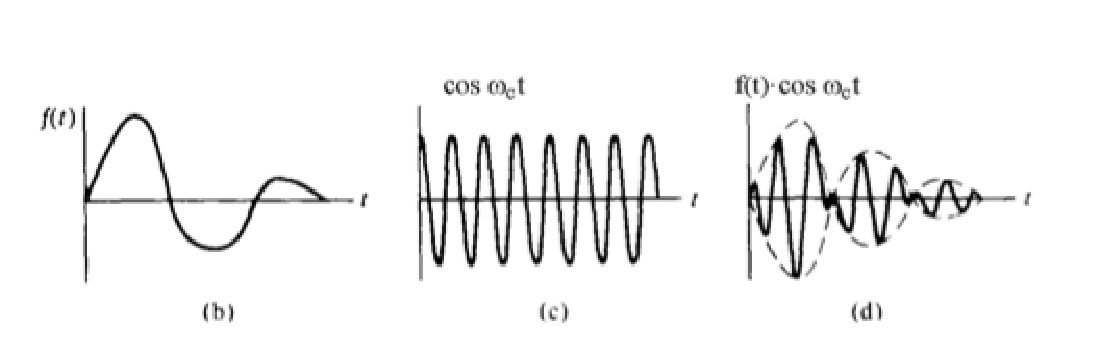
\includegraphics[scale=0.7, trim = 0cm 0cm 0cm 0cm, clip]{./Bilder/AMohneTraeger}
                    \caption{Amplitudenmodulation ohne träger}
                    \label{fig:AMohneTraeger}
                    \cite{AMohnetraeger}
            \end{figure}
    
            Um dieses modulierte Signal am Empfänger wieder zu demodulieren wird es noch ein weiteres mal mit dem
            Trägersignal multipliziert und anschließend Tiefpassgefiltert. Welche Auswirkung das hat zeigt folgendes
            Bild.
            
            \begin{figure}[H]
            \centering
                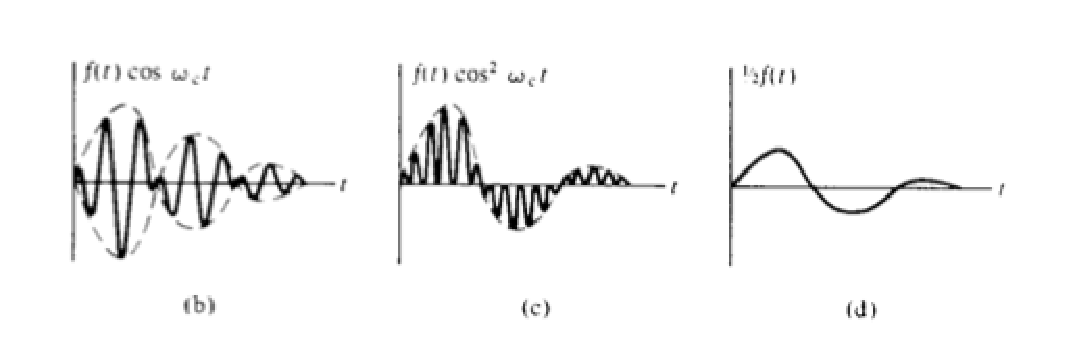
\includegraphics[scale=0.7, trim = 0cm 0cm 0cm 0cm, clip]{./Bilder/AMohnetraegerdemodulation}
                    \caption{Amplitudendemodulation ohne Träger}
                    \cite{AMdemodulation}
            \end{figure}
    
            Die Gesamte Übertragungsstecke der Amplitudenmodulation ohne Träger ist hier zu sehen.
            
            \begin{figure}[H]
            \centering
                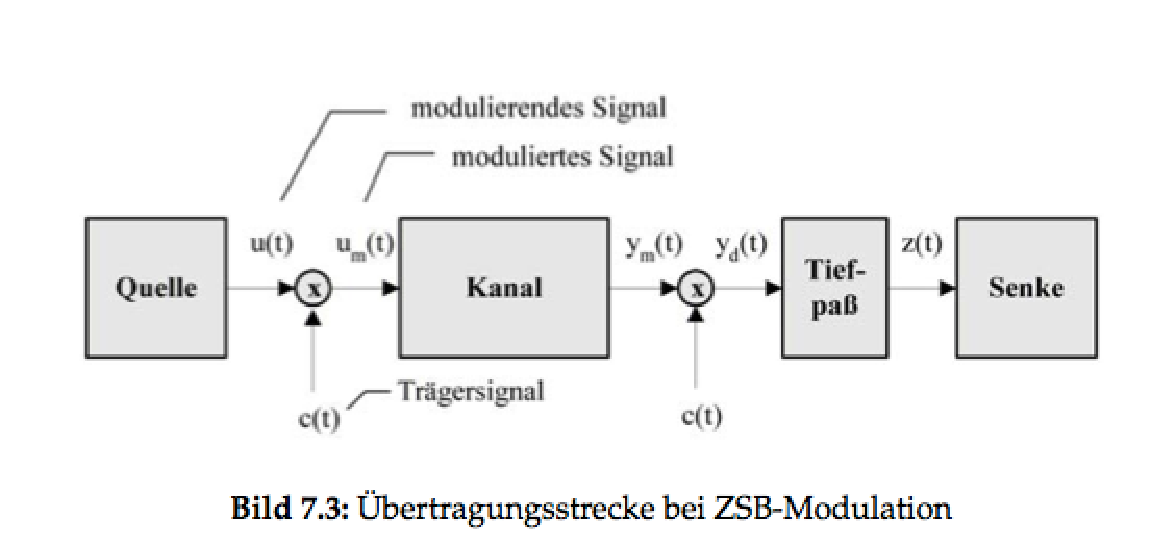
\includegraphics[scale=0.7, trim = 0cm 0cm 0cm 0cm, clip]{./Bilder/uebertragungsstreckeAMohnetraeger}
                    \caption{Übertragungsstrecke AM ohne Träger}
                    \cite{AMohneUeber}
            \end{figure}
             
             Damit diese Modulation jedoch fehlerfrei funktioniert wird am
             Empfänger das kohärente Trägersignal benötigt. Das Bedeutet, dass das Trägersignal in exakt der 
             selben Phase und Frequenz am Empfänger vorhanden sein muss. 
             Ist das nicht der Fall kommt es zur Verfälschung des Nutzsignals bei der Demodulation.\\
             Da das jedoch schwer zu realisieren ist wurde die zweite art der Amplitudenmodulation entwickelt:
             die Amplitudenmodulation mit Träger.
             
            
		\end{quote}
		
		\subsubsection{Amplitudenmodulation mit Träger}
		\begin{quote}
			Bei der Amplitudenmodulation mit Träger wird das Nutzsignal $u(t)$ bevor es mit dem Trägersignal $c(t)$
			multipliziert wird mit einem Offset versehen.
			
			\begin{figure}[H]
            \centering
                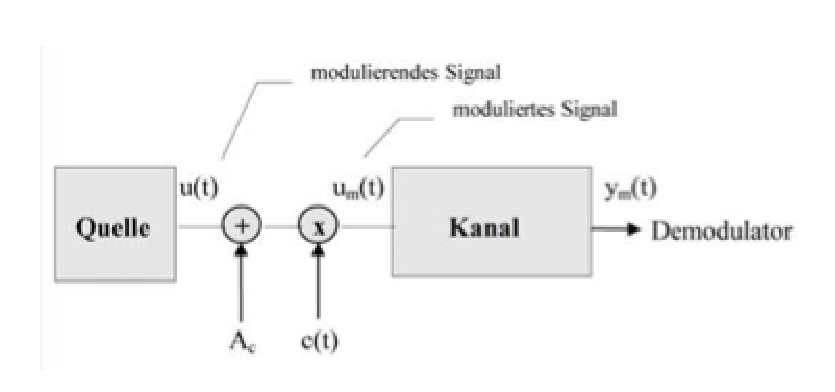
\includegraphics[scale=0.7, trim = 0cm 0cm 0cm 0cm, clip]{./Bilder/AMmitTraeger}
                    \caption{Amplituden Modulation mit Träger}
                    \cite{AMmitUeber}
            \end{figure}
            
            Für die Amplitude des modulierten Signals bedeutet das :
            
            \begin{equation*}
                \begin{split}
                    A_c [u(t)] = A + k \cdot u(t)
                \end{split}
            \end{equation*}
            
            Diese Art der Modulation hat folgende auswirkungen auf das Signal:
            
            \begin{figure}[H]
            \centering
                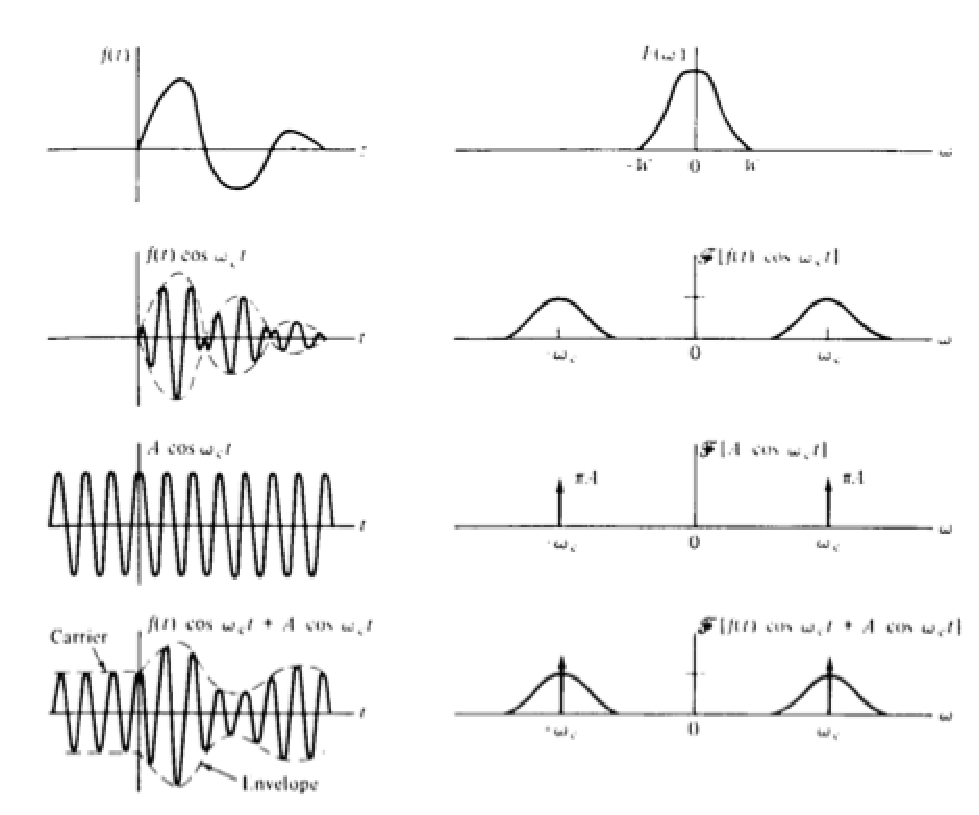
\includegraphics[scale=0.7, trim = 0cm 0cm 0cm 0cm, clip]{./Bilder/AMmittraegersignal}
                    \caption{Amplituden}
                    \cite{AMmitUeber}
            \end{figure}
            
            Für die Demodulation stehen bei diesem Verfahren zwei Möglichkeiten zur verfügung. Einerseits dieselbe
            Demodulation wie oben schon beschrieben, die erneute multiplikation mit dem Trägersignal.\\
            Andererseits lässt sich dieses Signal auch demodulieren indem das Signal gleichgerichtet wird und
            anschließend der Offset entfernt wird Außerdem muss auch dieses Signal Tiefpassgefiltert werden. Der Vorteil
            dieser zweiten Methode ist, dass sie sehr viel einfacher auf der Empfängerseite zu realisieren ist als die erst 
            Art der Demodulation.
    
		      
		\end{quote}
        
        
    \end{quote}
    
    \subsection{Vorbereitungsaufgabe}
    \begin{quote}
        Als Vorbereitung für die Messungen zum Thema Amplitudenmodulation haben wir mit Hilfe von Matlab verschiedene
        Signalformen simuliert und anschließend Amplituden moduliert.\\
        Dazu haben wir als Nutzsignal jeweils ein Rechtecksignal, ein Dreiecksignal sowie ein Cosinussignal mit
        einer Amplitude (von Nulldurchgang zum Spitzenwert) von $1V$, einer Frequenz von $100 Hz$ und einem Offset von
        $1V$ erzeugt.
        Zusätzlich haben wir noch ein Trägersignal mit der selben Amplitude aber mit einer Trägerfrequenz von $2000 Hz$ erstellt.\\
        Anschließend haben wir die drei Nutzsignale Amplitudenmoduliert indem wir sie jeweils mit dem Tägersignal
        multipliziert haben.\\
        Zur Analyse haben abschließende diese modulierten Signale sowie ihre Amplituden- und Phasengänge plotten
        lassen.\\
        In der Auswertung werden wir diese Ergebnisse anschließend mit den gemessenen Ergebnissen vergleichen.
    \end{quote}
    
    \subsection{Durchführung}
    \begin{quote}
    	\subsubsection{Signalerzeugung und Modulation}
    	\begin{quote}
    	Als Basisbandsignal generierten wir ein mittelwertfreier Sinus,
    	der eine Frequenz von $100 Hz$ und eine Amplitude von $1 V$ besaß. Dazu wurde noch
    	ein Offset von einem Volt addiert, welches wir mit dem Adder-Modul und der
    	Quelle Variable DCV verwirklicht haben. Somit hatte unser Basisbandsignal
    	keinen Nulldurchgang mehr. Mit den Verstärkerknöpfen g und G wurde die
    	Summe vom Sinus und Offset korrekt eingestellt und am Oszilloskop
    	korrigiert.\\
    	Nachdem unser Nutzsignal erstellt wurde, führten wir die Modulation anhand
    	einer Multiplikation mit dem Multiplier-Modul durch. Als Trägersignal
    	verwendeten wir dabei den $2kHz$-Sinus des Master-Signal-Moduls.\\
    	Nach der Untersuchung des Sinus-Basisbandsignals, wurde die Modulation auf
    	gleiche Weise noch mit dem Rechteck- und dem Dreiecksignal durchgeführt.
    	Die Ergebnisse aus dem Praktikum und der Vergleich mit den Ergebnissen aus
    	der Vorbereitungsaufgabe ist in der Auswertung zu finden.
    	\end{quote}
    	
    	\vspace{1em}
    	
    	\subsubsection{Synchrone Demodulation}
    	\begin{quote}
    	Nach der Amplitudenmodulation wurden die modulierten Signale auch
    	synchron demoduliert. Dies ermöglichten wir mithilfe des zweiten
    	Multiplier-Moduls und indem wir das Trägersignal erneut auf das modulierte
    	Signal multiplizierten. In einem Plot kann man sehen, dass das
    	Empfangssignal vierfache Amplitude besitzt als das Sendesignal.
    	Diese Abweichung korrigierten wir anhand eines Tiefpasses nach der
    	Demodulation.
    	
    	Ist das alles richtig so? was hatte Michael Tok denn gesagt? Auf jeden Fall
    	haben wir Messwerte zu demodulierten und demoduliert gefilterten Signalen.
    	Bei den gefilterten sind deutlich kleinere Amplituden zu sehen.
		\end{quote}    
    
    \end{quote}
    
    \subsection{Auswertung}
    \begin{quote}
        
        Hier kann man die Ergebnisse der Amplitudenmodulation sehen. Alle Nutzsignale, sowohl simuliert als auch
        gemessen, hatten eine Frequenz von $100 Hz$, eine Amplitude von $1 V$ und einen Offset von ebenfalls $1 V$. Das
        Trägersignal war ein $2 kHz$-Sinus.
        
        \subsubsection{modulierte Signale}
		\begin{quote}
		  
		  Wir erwaten bei den drei Signalen nach der modulation das ursprüngliche Nutzsignal in als Einhüllende des
		  modulierten Signals wiederzufinden. Innerhalb dieser Einhüllenden wird das $2kHz$ Trägersignal zu finden sein.
		  
            \begin{center}
                \begin{tabular}{ll}
    
                \hspace{-10em}
                    \begin{minipage}{0.6\textwidth}
    
                        \begin{figure}[H]
                            \label{fig:}
                            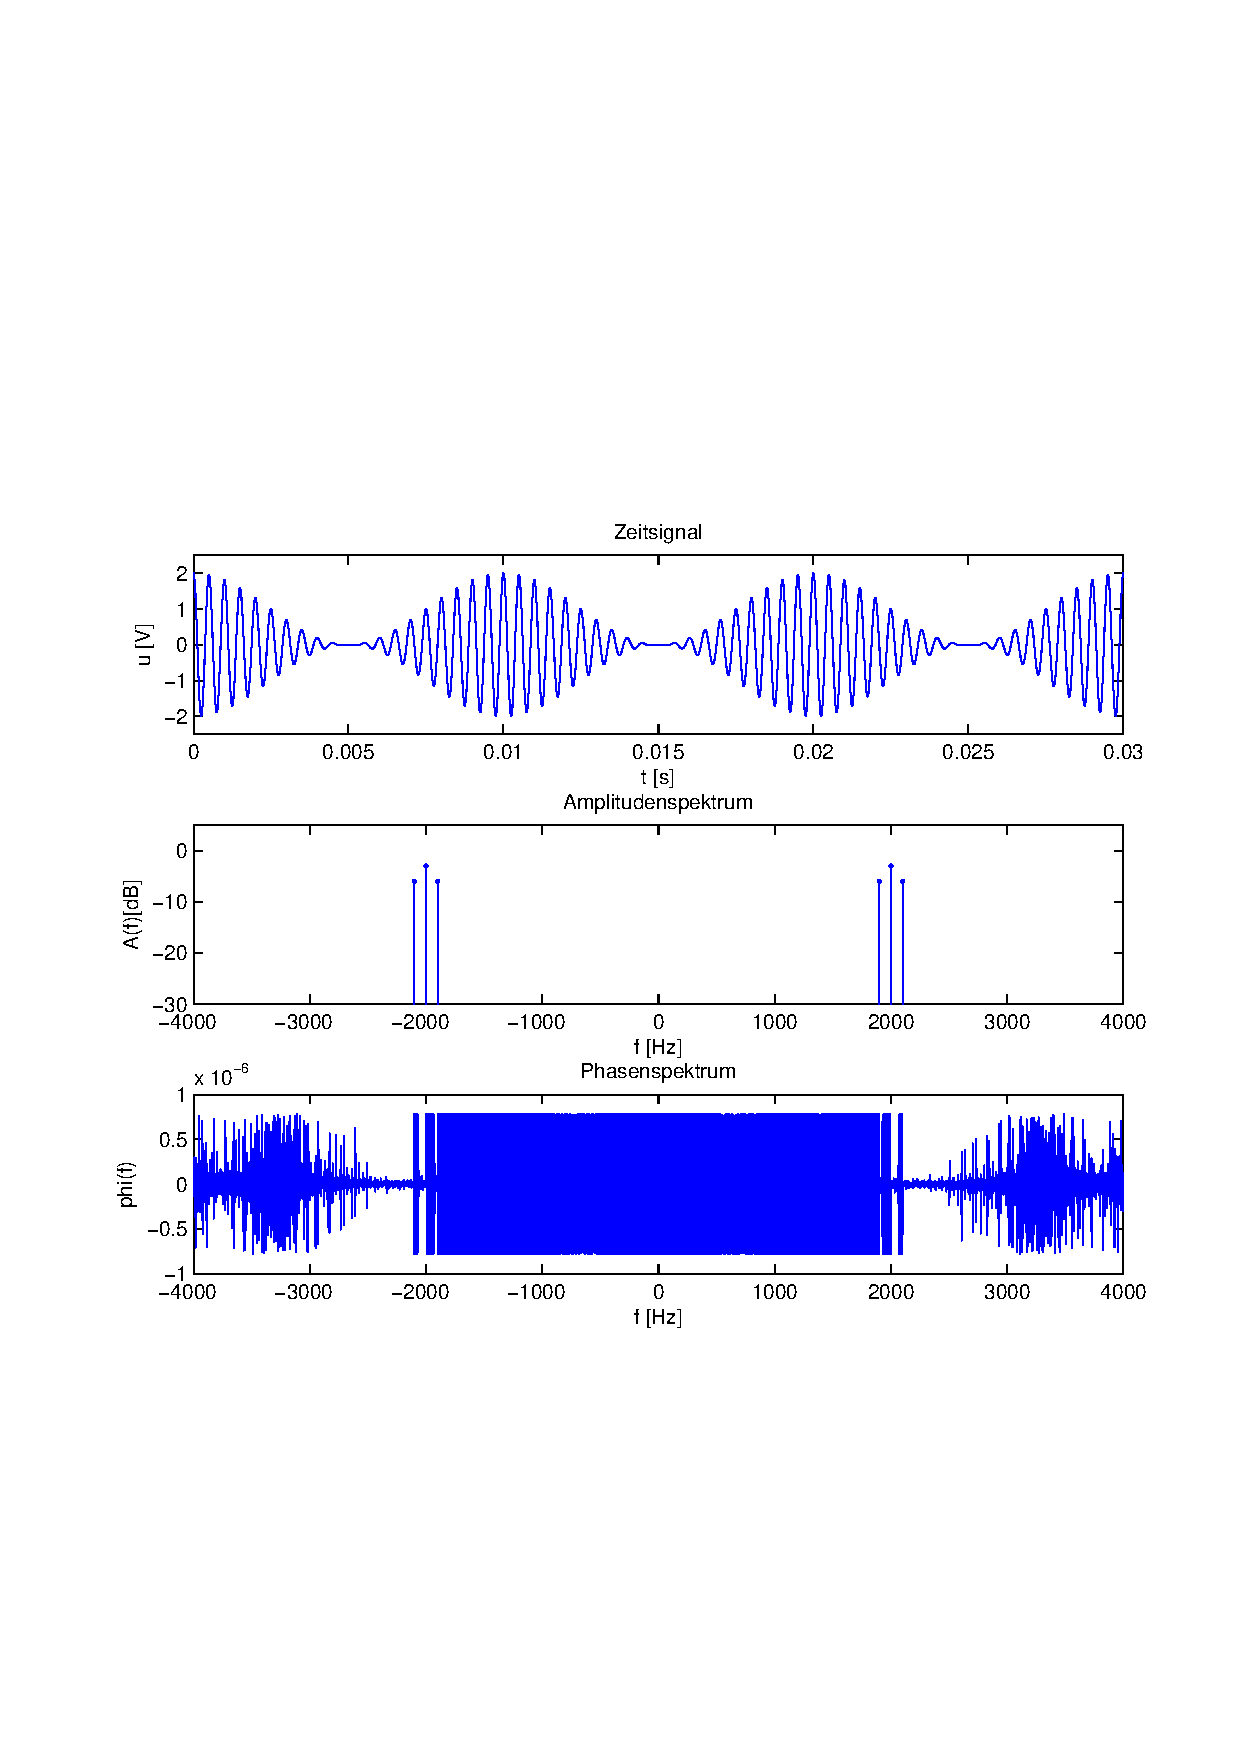
\includegraphics[scale=0.4, trim = 2cm 6.5cm 1.5cm
                            8.5cm, clip]{./Bilder/Cosinusmodsimuliert} %FIXME [width=640px,
                            % height=474px]
                            \caption{amplitudenmoduliertes Cosinussignal simuliert}
                        \end{figure}
    
                    \end{minipage}
                    \begin{minipage}{0.6\textwidth}
    
                         \begin{figure}[H]
                            \label{fig:}
                            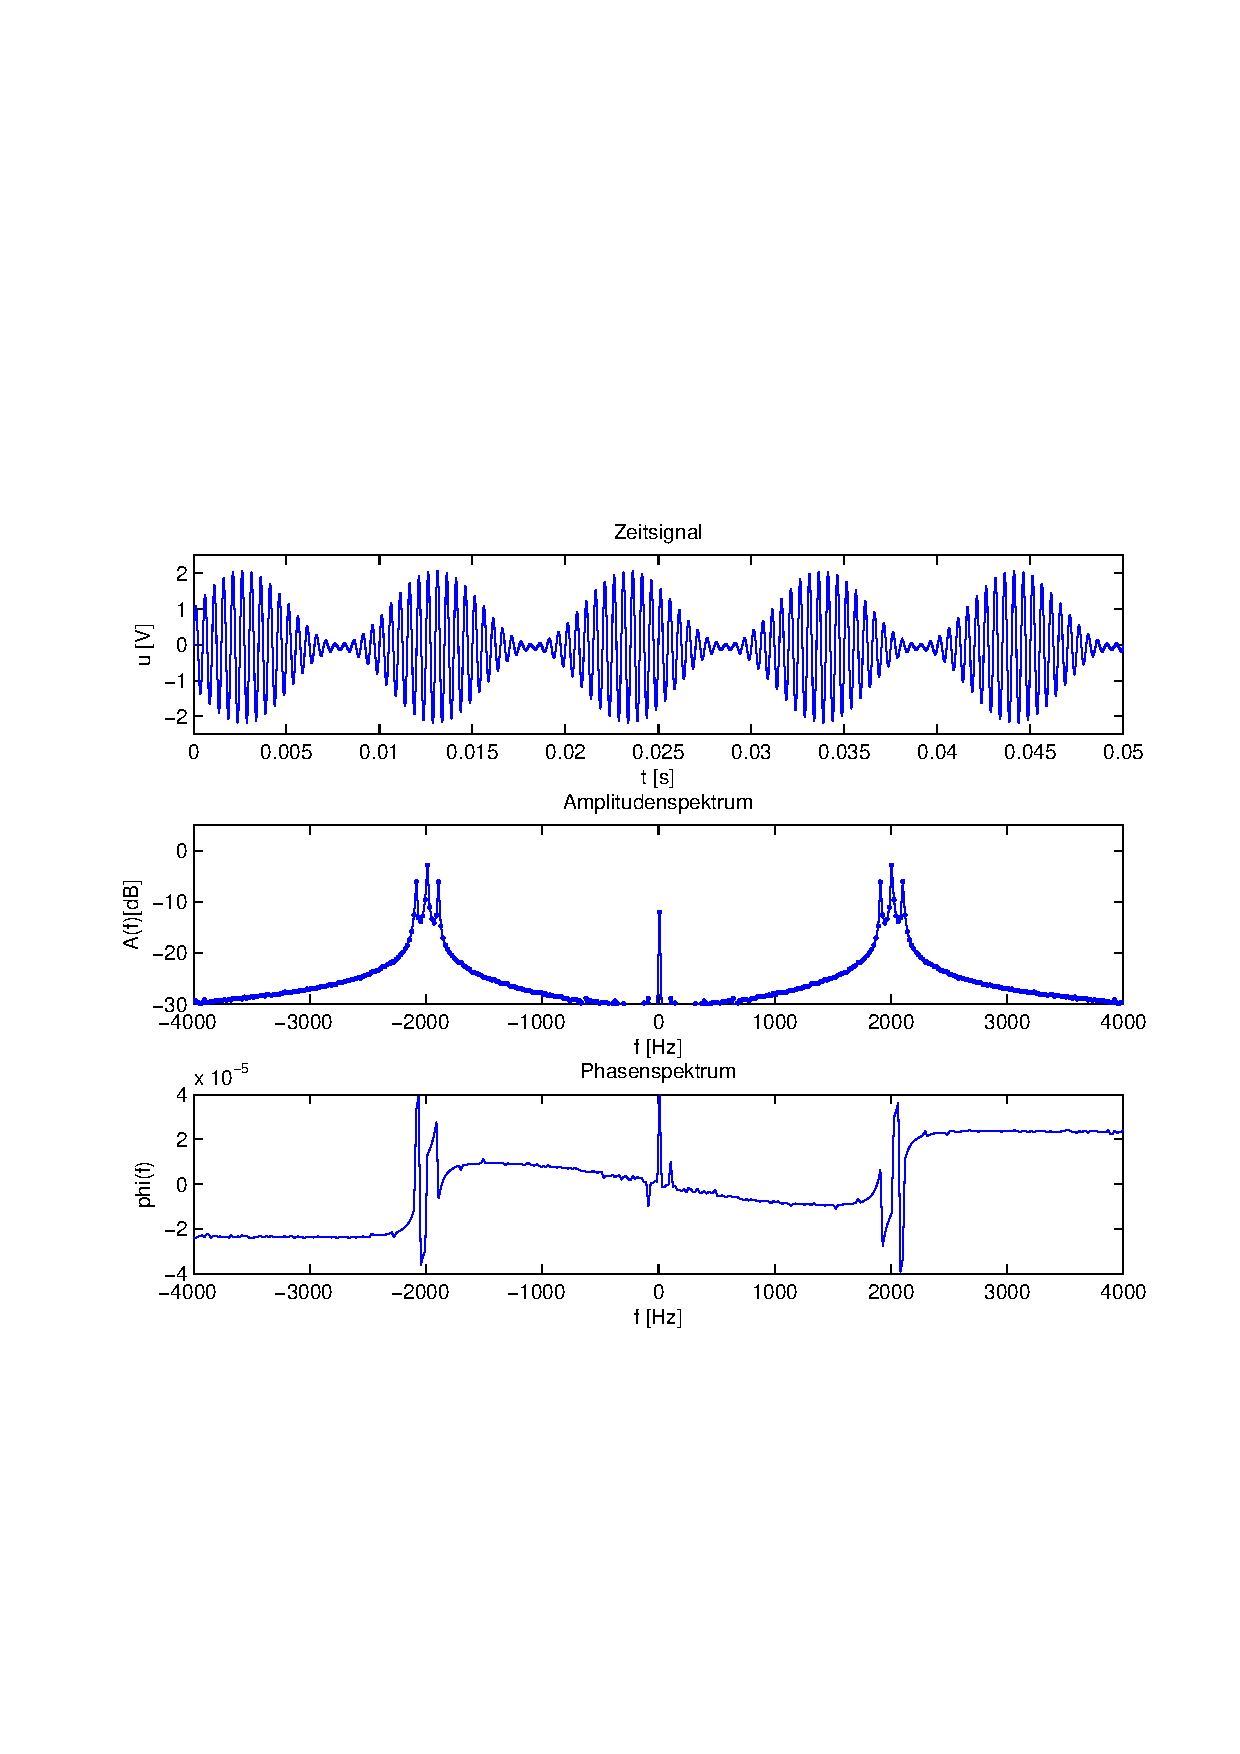
\includegraphics[scale=0.4, trim = 2cm 6.5cm 1.5cm
                            8.5cm, clip]{./Bilder/Cosinusmodgemessen} %FIXME
                            % [width=640px, height=474px]
                            \caption{amplitudenmoduliertes Cosinussignal gemessen}
                        \end{figure}
                   \vspace{-1.5em}
    
                    \end{minipage}
    
                \end{tabular}
                \end{center}
                
                        \begin{center}
                \begin{tabular}{ll}
    
                \hspace{-10em}
                    \begin{minipage}{0.6\textwidth}
    
                        \begin{figure}[H]
                            \label{fig:}
                            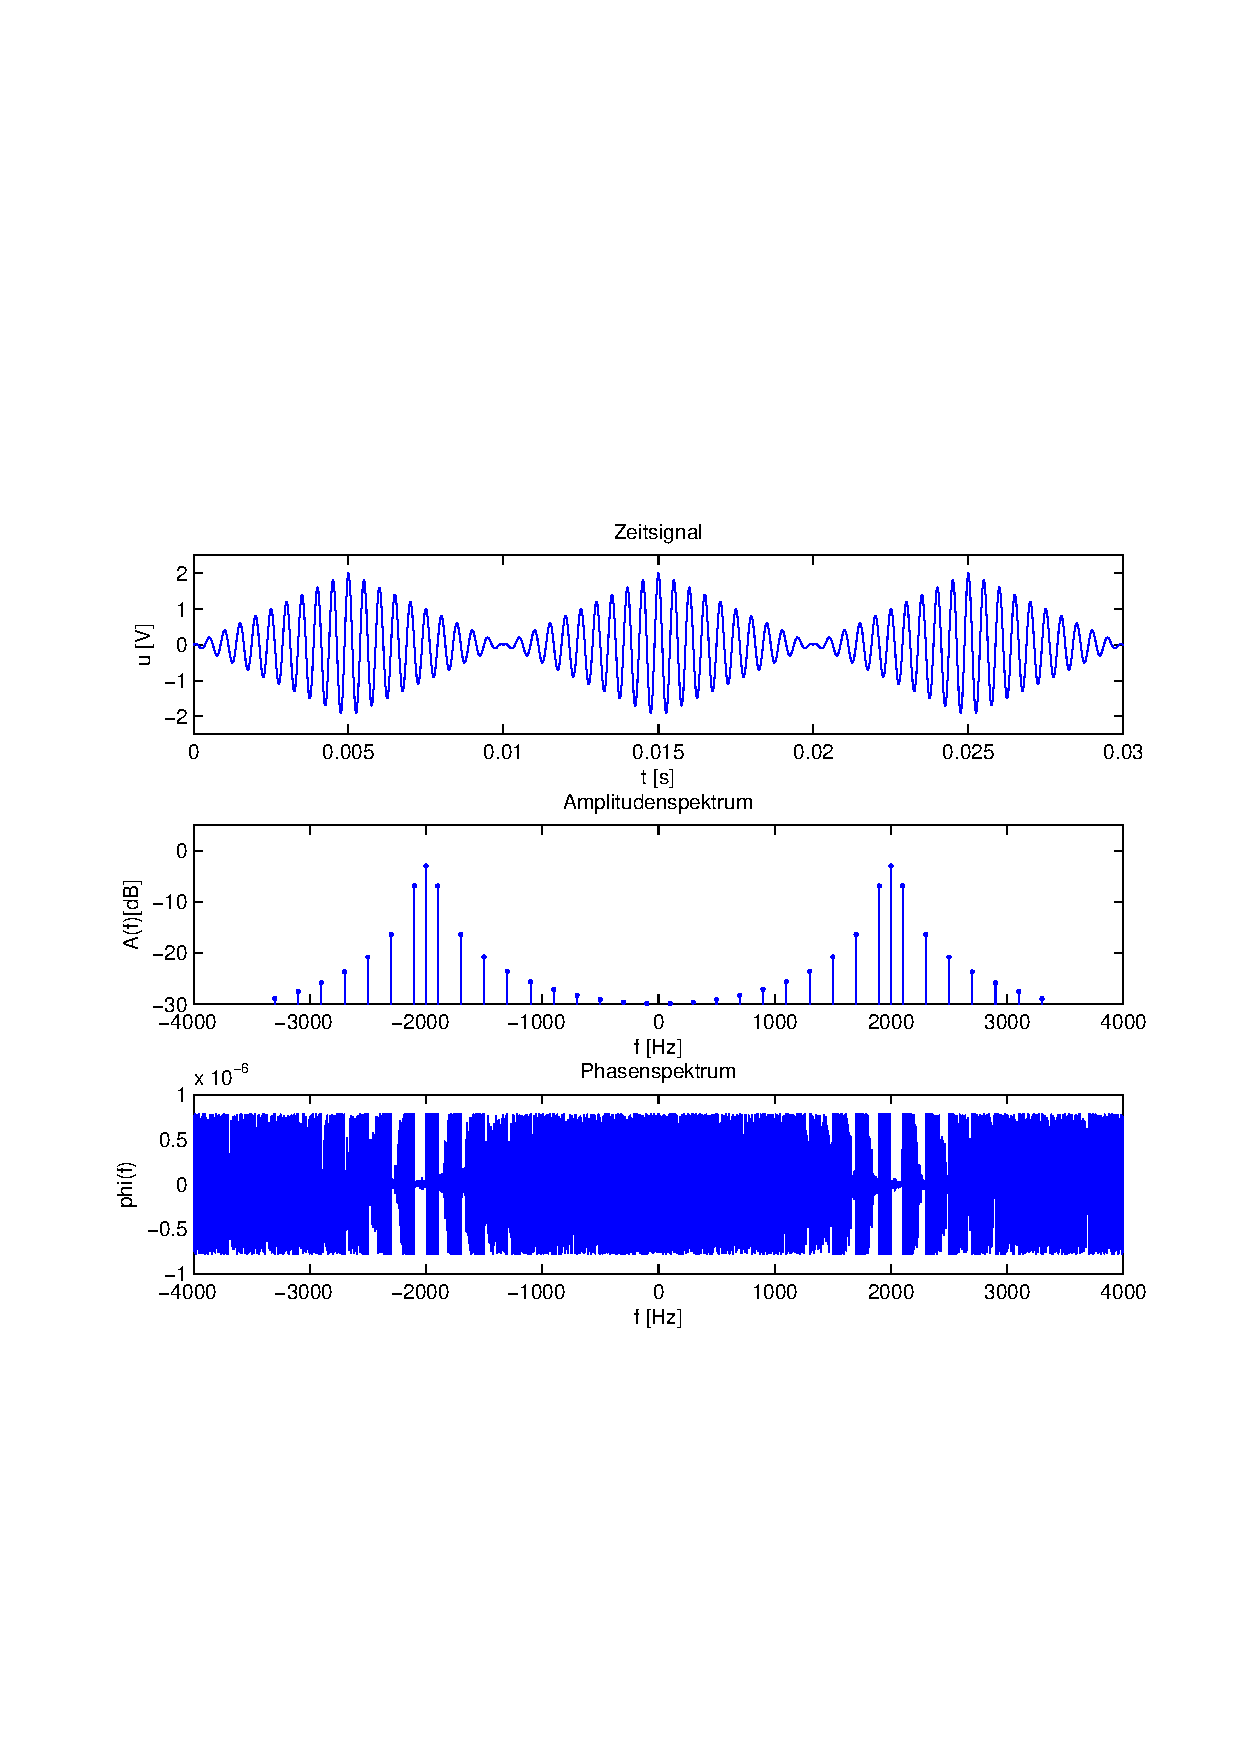
\includegraphics[scale=0.4, trim = 2cm 6.5cm 1.5cm
                            8.5cm, clip]{./Bilder/Dreieckmodsimuliert} %FIXME [width=640px,
                            % height=474px]
                            \caption{amplitudenmoduliertes Dreiecksignal simuliert}
                        \end{figure}
    
                    \end{minipage}
                    \begin{minipage}{0.6\textwidth}
    
                         \begin{figure}[H]
                            \label{fig:}
                            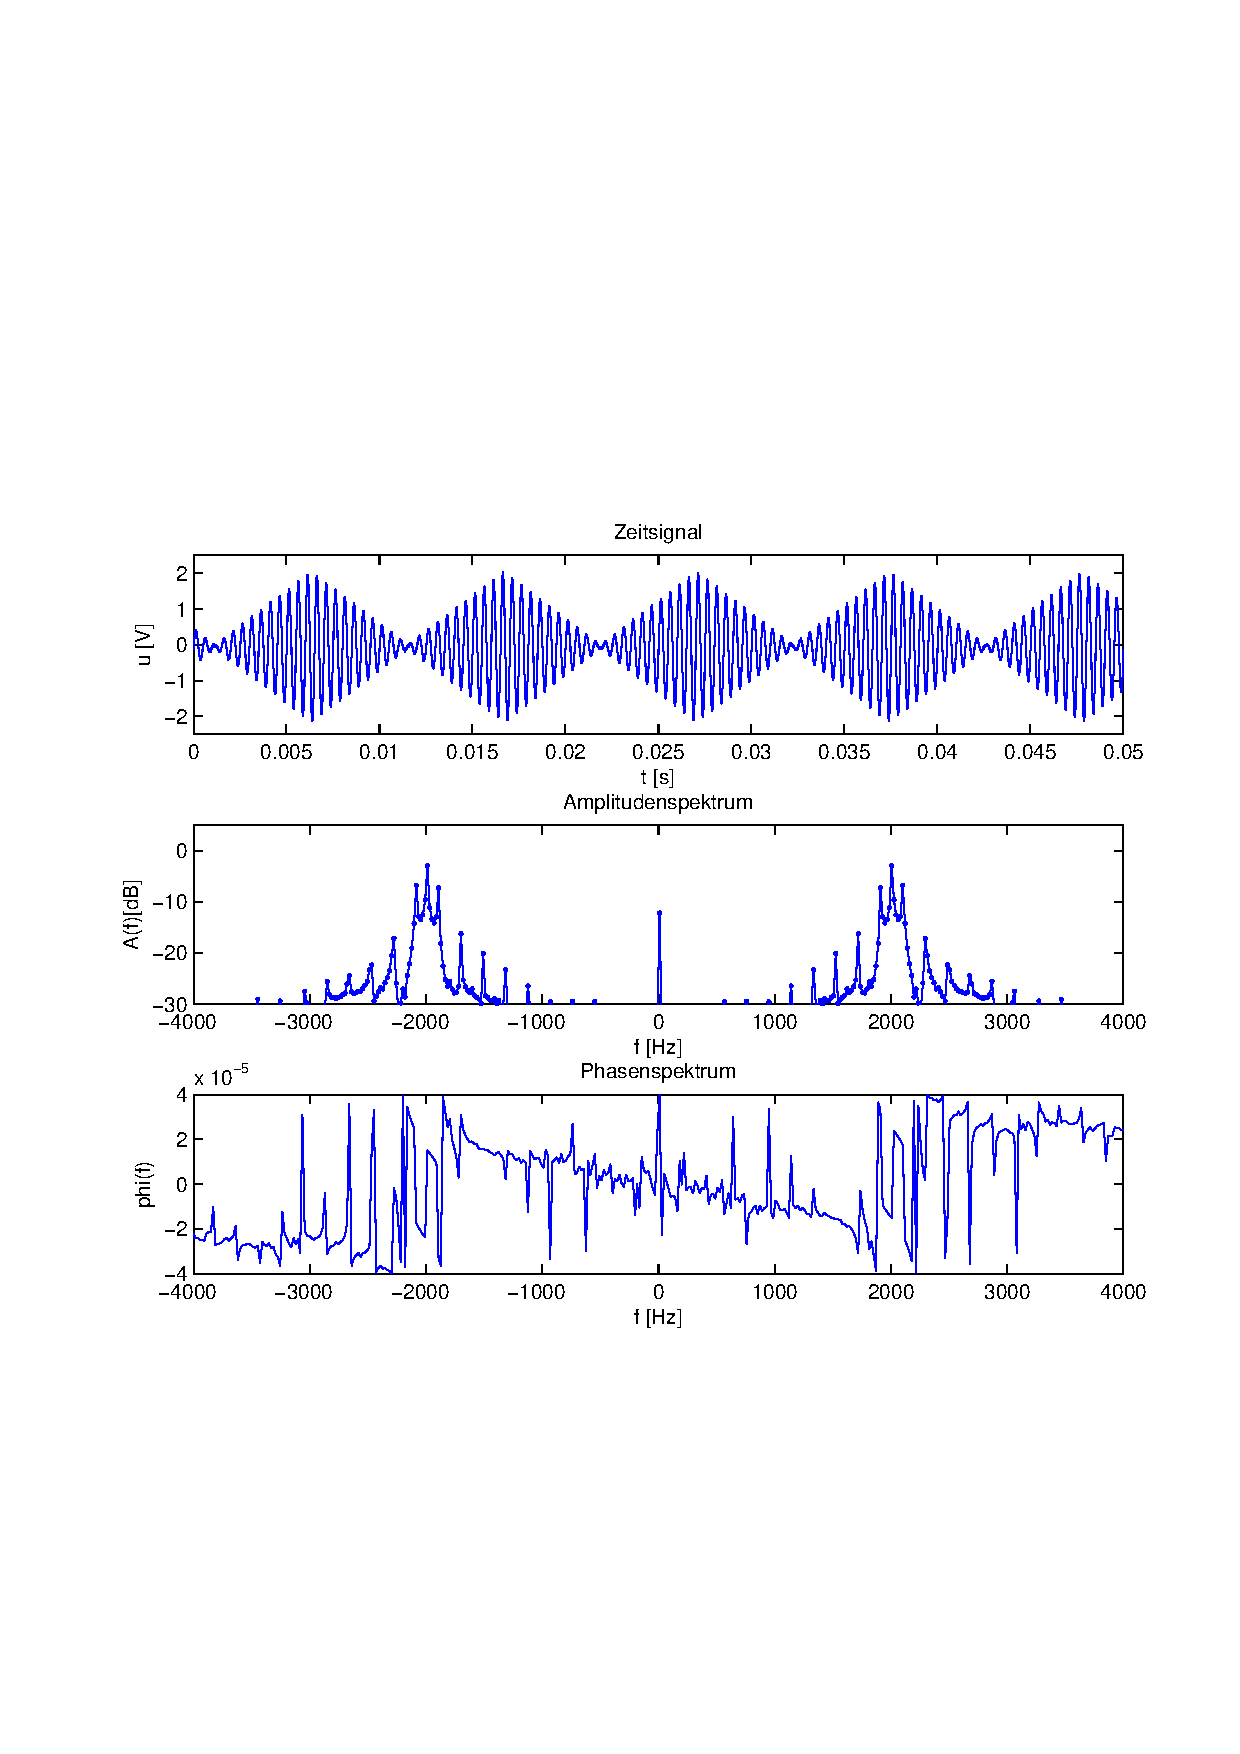
\includegraphics[scale=0.4, trim = 2cm 6.5cm 1.5cm
                            8.5cm, clip]{./Bilder/Dreieckmodgemessen} %FIXME
                            % [width=640px, height=474px]
                            \caption{amplitudenmoduliertes Dreiecksignal gemessen}
                        \end{figure}
                   \vspace{-1.5em}
    
                    \end{minipage}
    
                \end{tabular}
                \end{center}
                
                        \begin{center}
                \begin{tabular}{ll}
    
                \hspace{-10em}
                    \begin{minipage}{0.6\textwidth}
    
                        \begin{figure}[H]
                            \label{fig:}
                            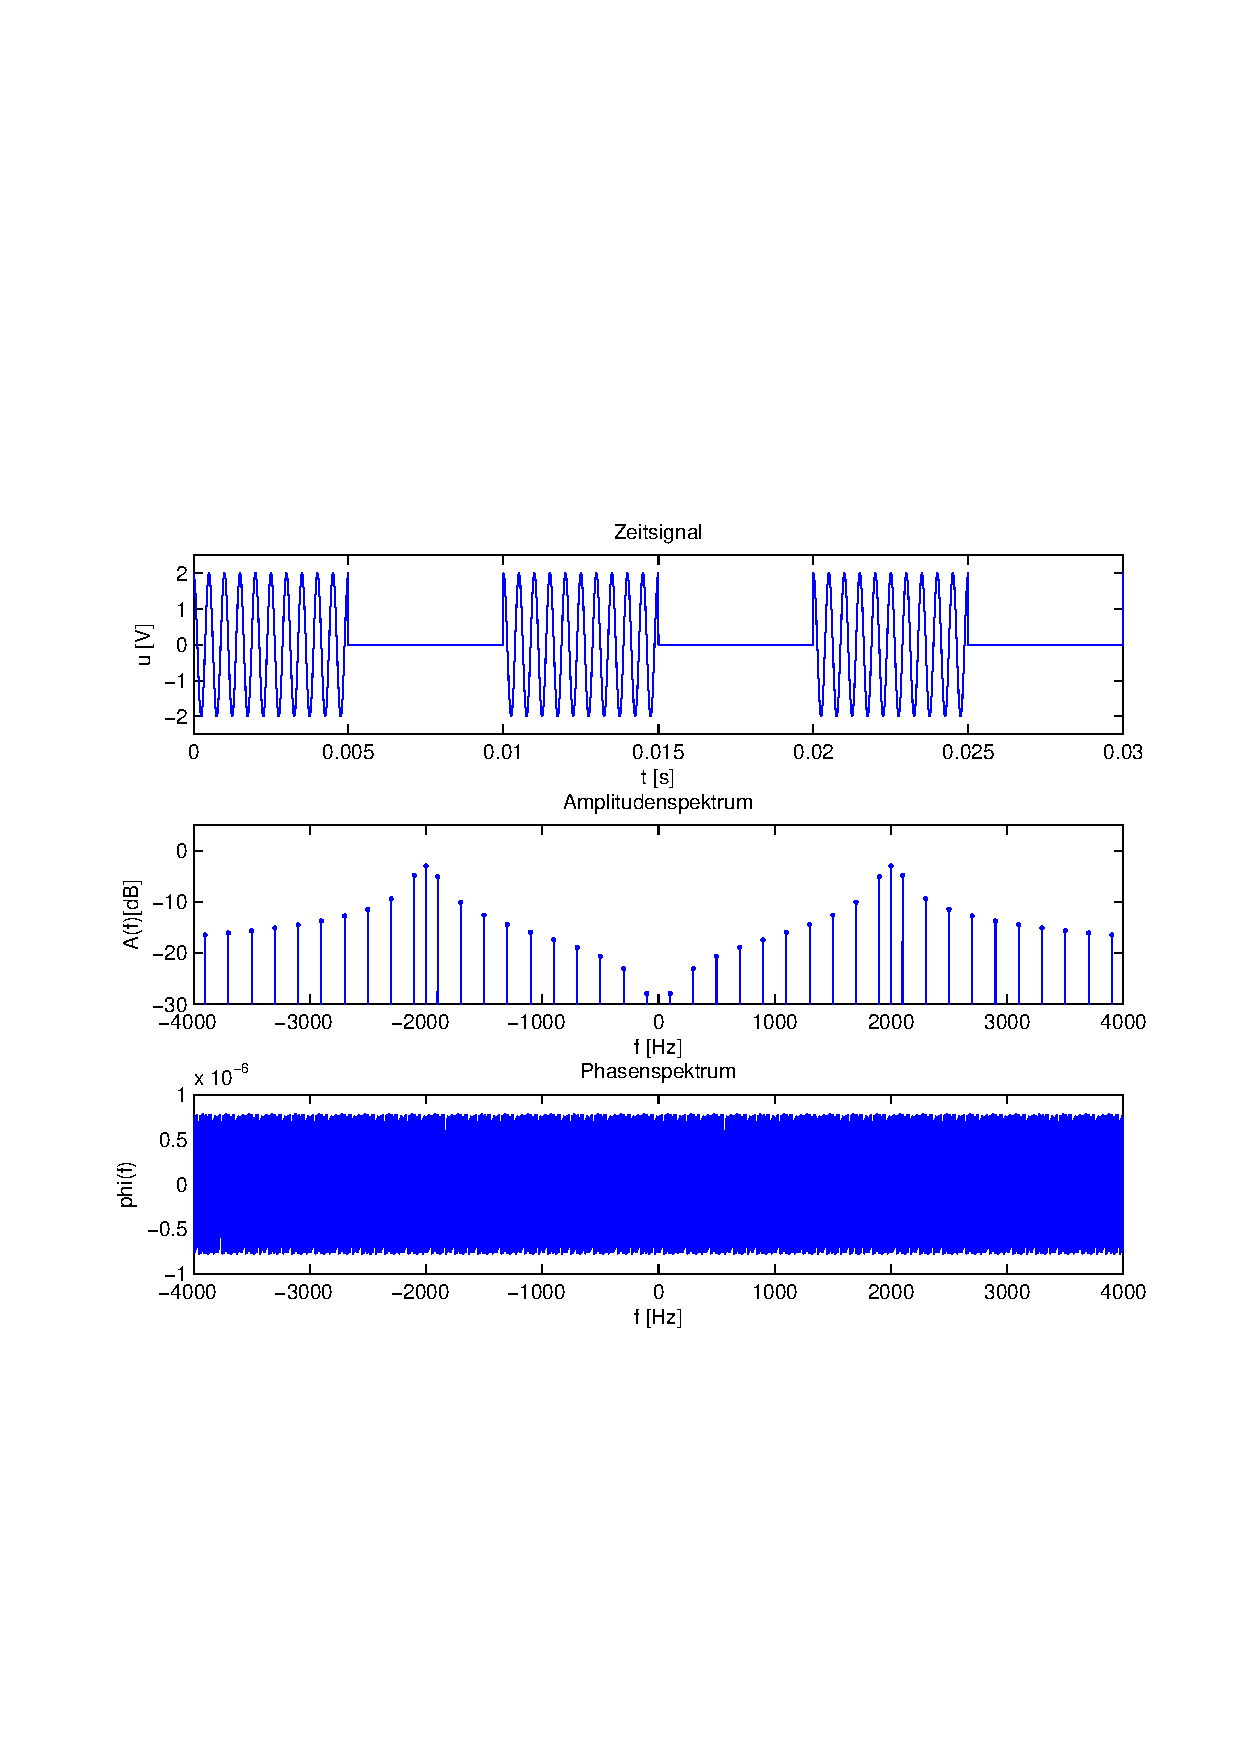
\includegraphics[scale=0.4, trim = 2cm 6.5cm 1.5cm
                            8.5cm, clip]{./Bilder/Rechteckmodsimuliert} %FIXME [width=640px,
                            % height=474px]
                            \caption{amplitudenmoduliertes Rechtecksignal simuliert}
                        \end{figure}
    
                    \end{minipage}
                    \begin{minipage}{0.6\textwidth}
    
                         \begin{figure}[H]
                            \label{fig:}
                            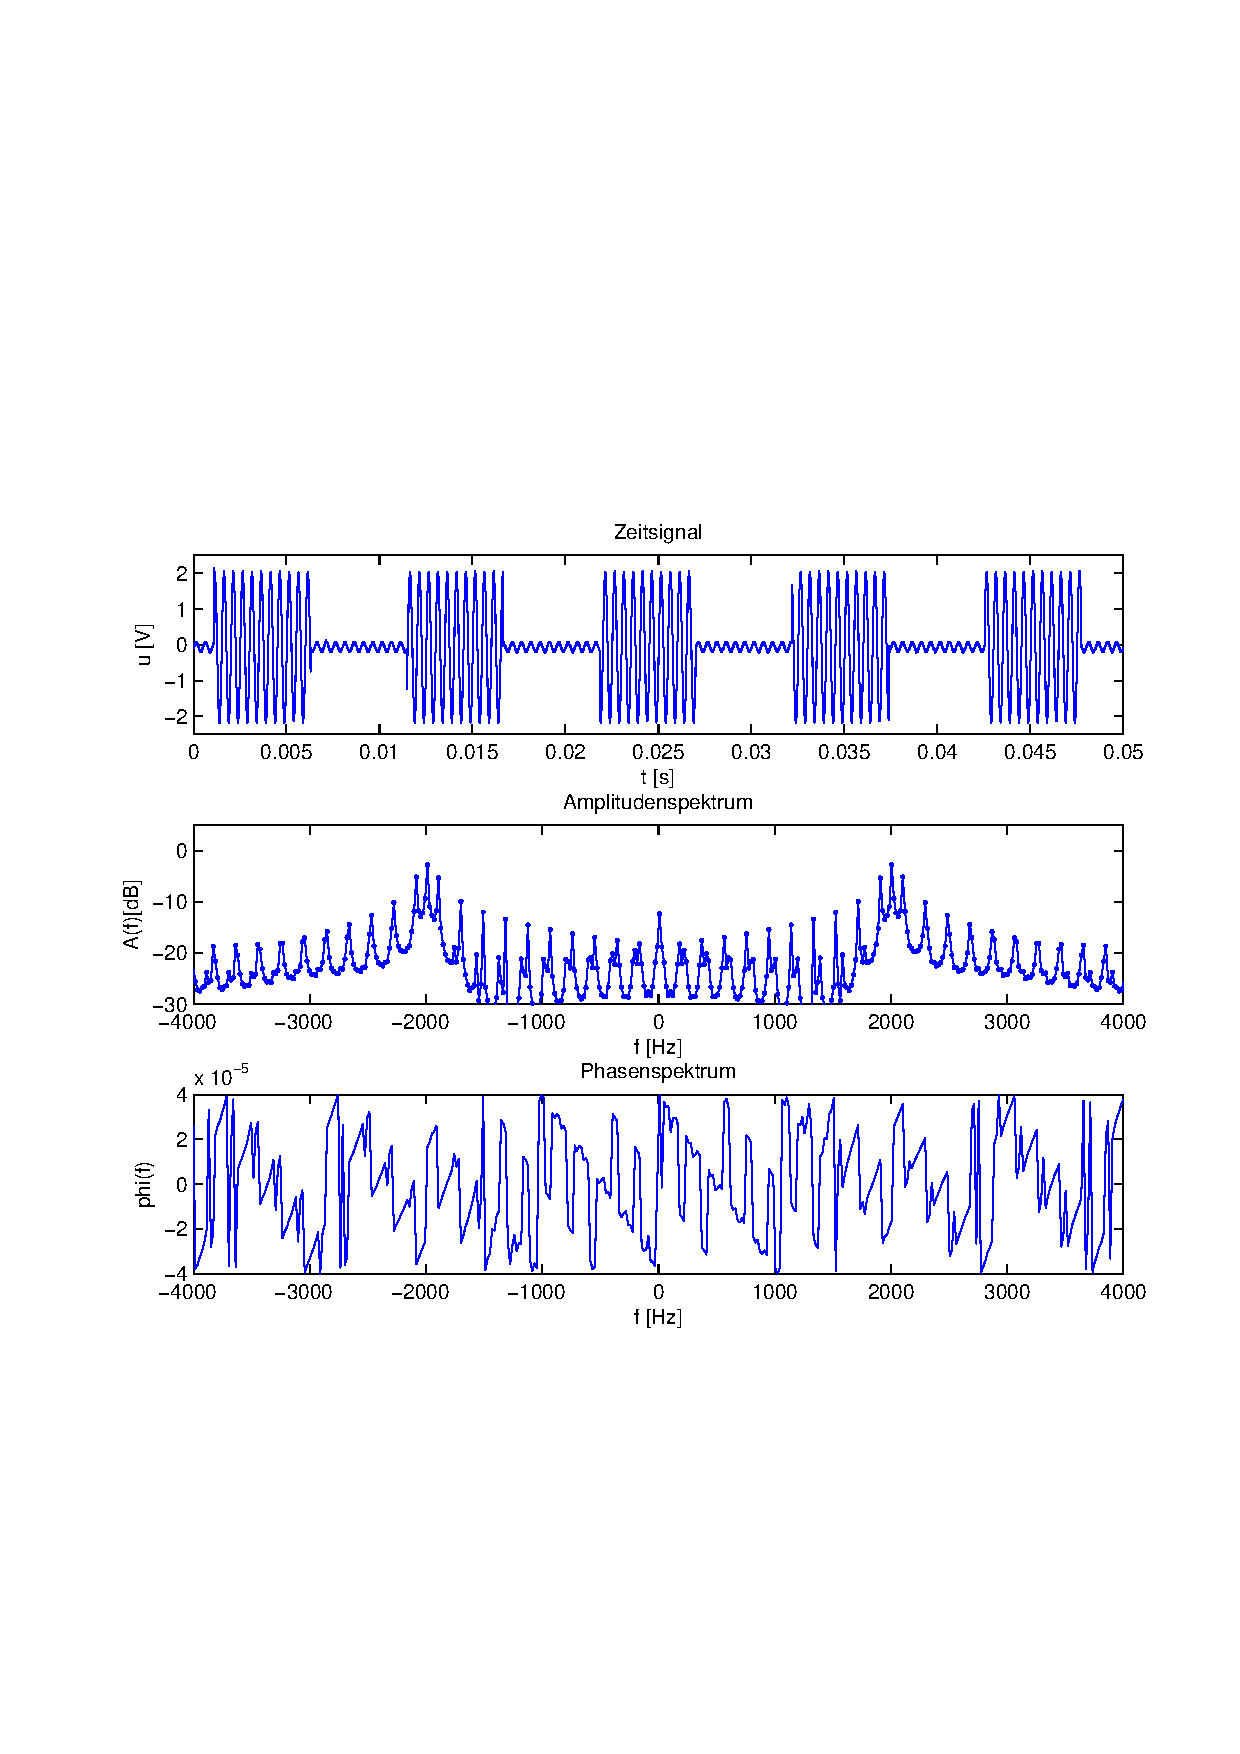
\includegraphics[scale=0.4, trim = 2cm 6.5cm 1.5cm
                            8.5cm, clip]{./Bilder/Rechteckmodgemessen} %FIXME
                            % [width=640px, height=474px]
                            \caption{amplitudenmoduliertes Rechtecksignal gemessen}
                        \end{figure}
                   \vspace{-1.5em}
    
                    \end{minipage}
    
                \end{tabular}
                \end{center}
                
                Unsere Erwartung bestätigt sich schon bei den in den Vorbereitungsaufgaben simulierten Signalen. Die
                original Cosinus-, Dreieck- und Rechteckförmigen Nutzsignale sind problemlos zu erkennen. Wobei zu
                beachten ist, dass es sich bei der Einhüllenden um mehr als nur das Nutzsignal handelt, da das Signal
                von $-2V$ bis $+2V$ alterniert. Erfreulich ist, dass sich auch die gemessenen modulierten Signale
                ziemlich eindeutig so ergeben wie wir es erwartet haben.\\
                Jedoch fallen auch einige Unterschiede in der Genauigkeit der Spektren der simulierten Signale im
                Verleich zu den gemessenen Signalen auf. Diese unterschiedliche Genauigkeit lässt sich sehr schon an dem
                Cosinussignal betrachten. Während das simulierte Spektrum ausschließlich $6$ Peaks bei $\pm 2000 Hz$
                besitzt kann man bei den gemessen Signalen neben diesen $6$ Peaks auch noch diverse andere Frequenzen
                erkennen. Da diese $6$ entsprechenden Peaks auch bei dem gemessene Signal besonders herausragen lässt
                sich sagen, dass es sich um die entscheidenden Frequenzen des Spektrums handels. Die weiteren Frequenzen
                sind auf Rauschen, ungenaue Einstellungen und andere Störungen bei der realen Messung zurückzuführen.\\
                Diese Vermutung wird auch durch das Rechtecksignal verstärkt. Während das simulierte Signal reine
                Nullabschnitte besitzt sind die entsprechenden Abschnitte bei dem gemessenen Signal durch sichtbare
                Welligkeit geprägt. Da diese Welligkeit auffallend wie das $2kHz$ Trägersignal aussieht liegt die
                Vermutung nahe, dass das Nutzsignal nicht exakt auf $0V$ runtergestellt war.
                  
                
			
		\end{quote}
            
        \subsubsection{demodulierte Signale ohne Tiefpass}
		\begin{quote}
            Bei der Demodulation wurde das Trägersignal ein zweites mal auf das
            bereits modulierte Nutzsignal multipliziert. Die Synchronität war
            dadurch gewährleistet, dass das selbe Trägersignal wie bei der
            Modulation verwendet wurde.\\
            Hier werden die ursprünglichen Sendesignalen mit den
            demodulierten Empfangssignalen verglichen:
            
                \begin{center}
                \begin{tabular}{ll}
    
                \hspace{-14em}
                    \begin{minipage}{0.6\textwidth}
    
                        \begin{figure}[H]
                            \label{fig:}
                            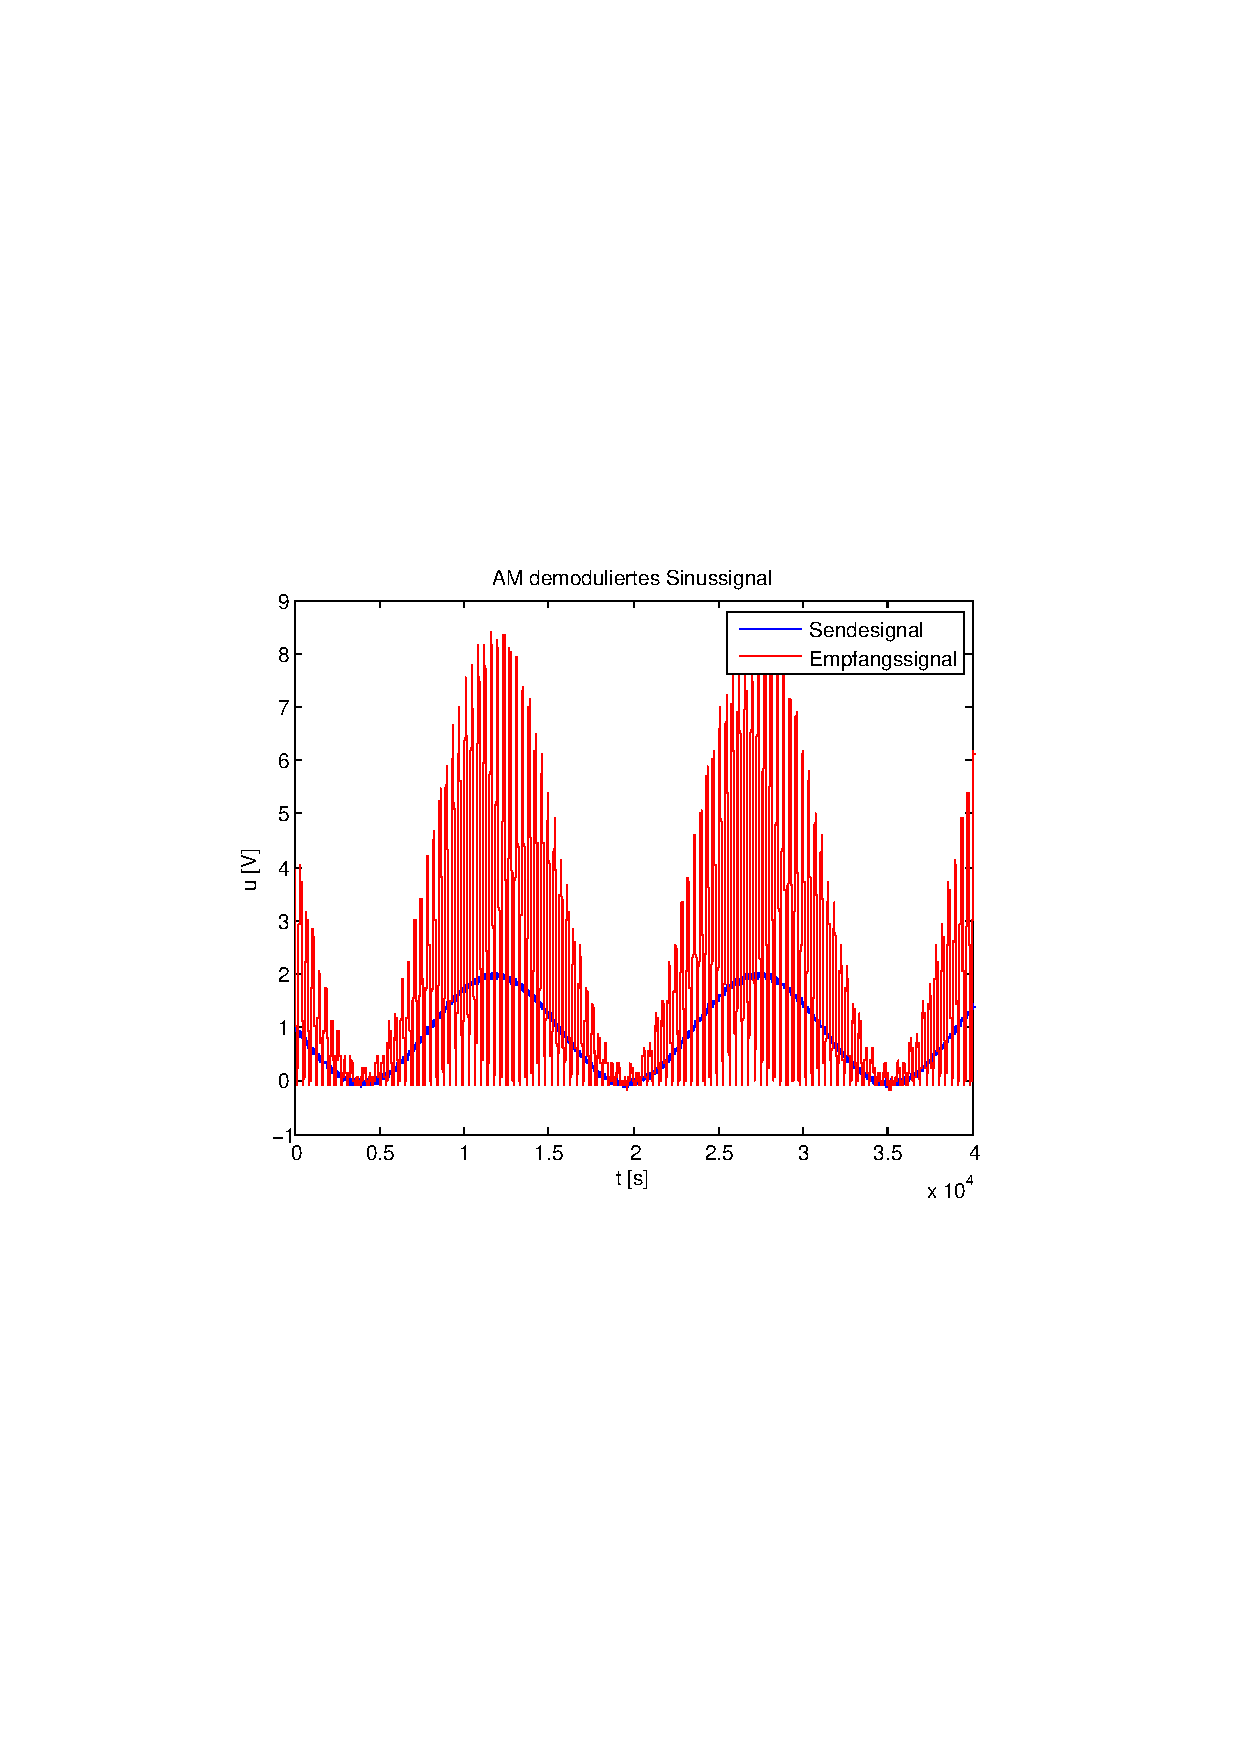
\includegraphics[scale=0.5, trim = 4cm 9.5cm 3.5cm
                        9.5cm, clip]{./Bilder/synchDemod_sinus} %FIXME
                            % [width=640px, height=474px]
                            \caption{amplitudendemoduliertes Sinussignal}
                        \end{figure}
    
                    \end{minipage}
                    \begin{minipage}{0.6\textwidth}
    
                         \begin{figure}[H]
                            \label{fig:}
                            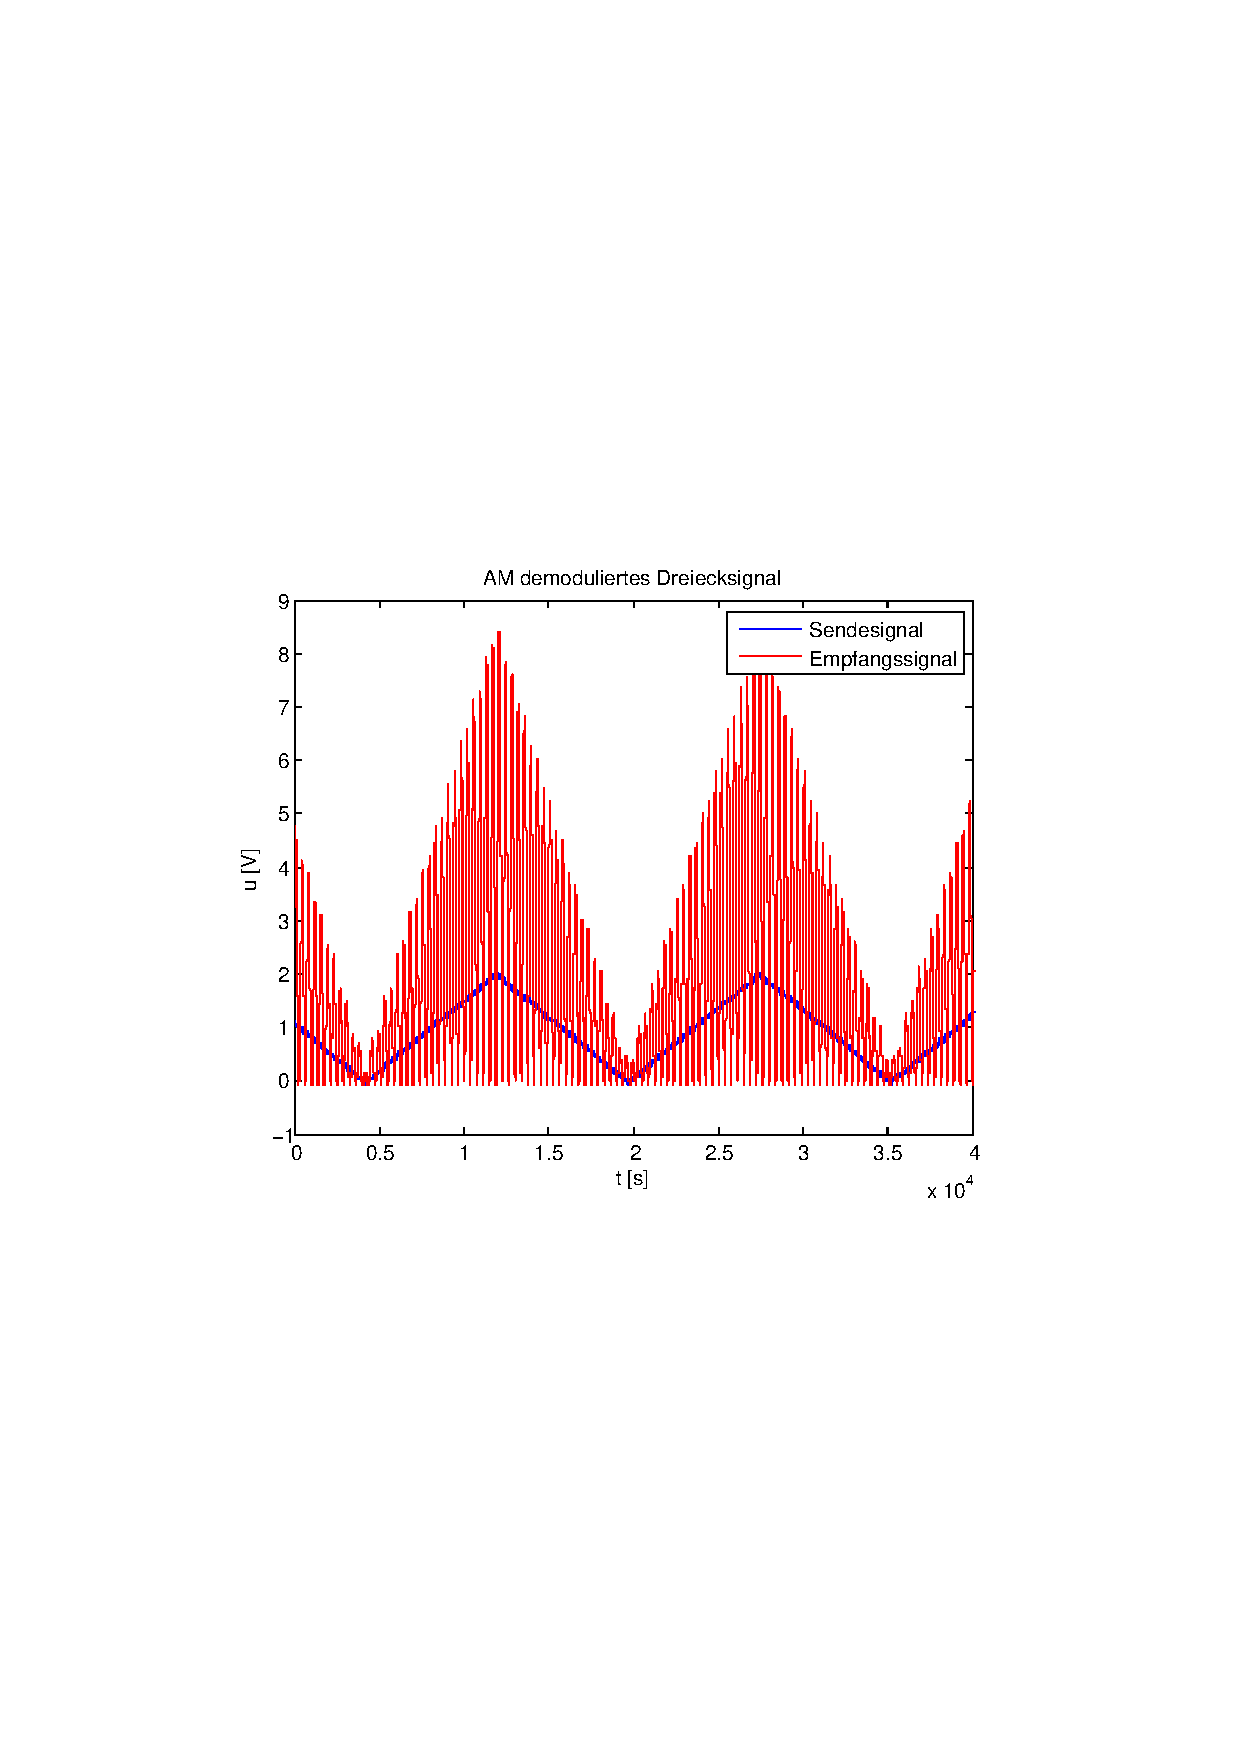
\includegraphics[scale=0.5, trim = 4cm 9.5cm 3.5cm
                        9.5cm, clip]{./Bilder/snychDemod_dreieck.pdf} %FIXME
                            % [width=640px, height=474px]
                            \caption{amplitudendemoduliertes Dreiecksignal}
                        \end{figure}
                   \vspace{-1.5em}
    
                    \end{minipage}
    
                \end{tabular}
                \end{center}
                
                 \begin{figure}[H] \centering
                        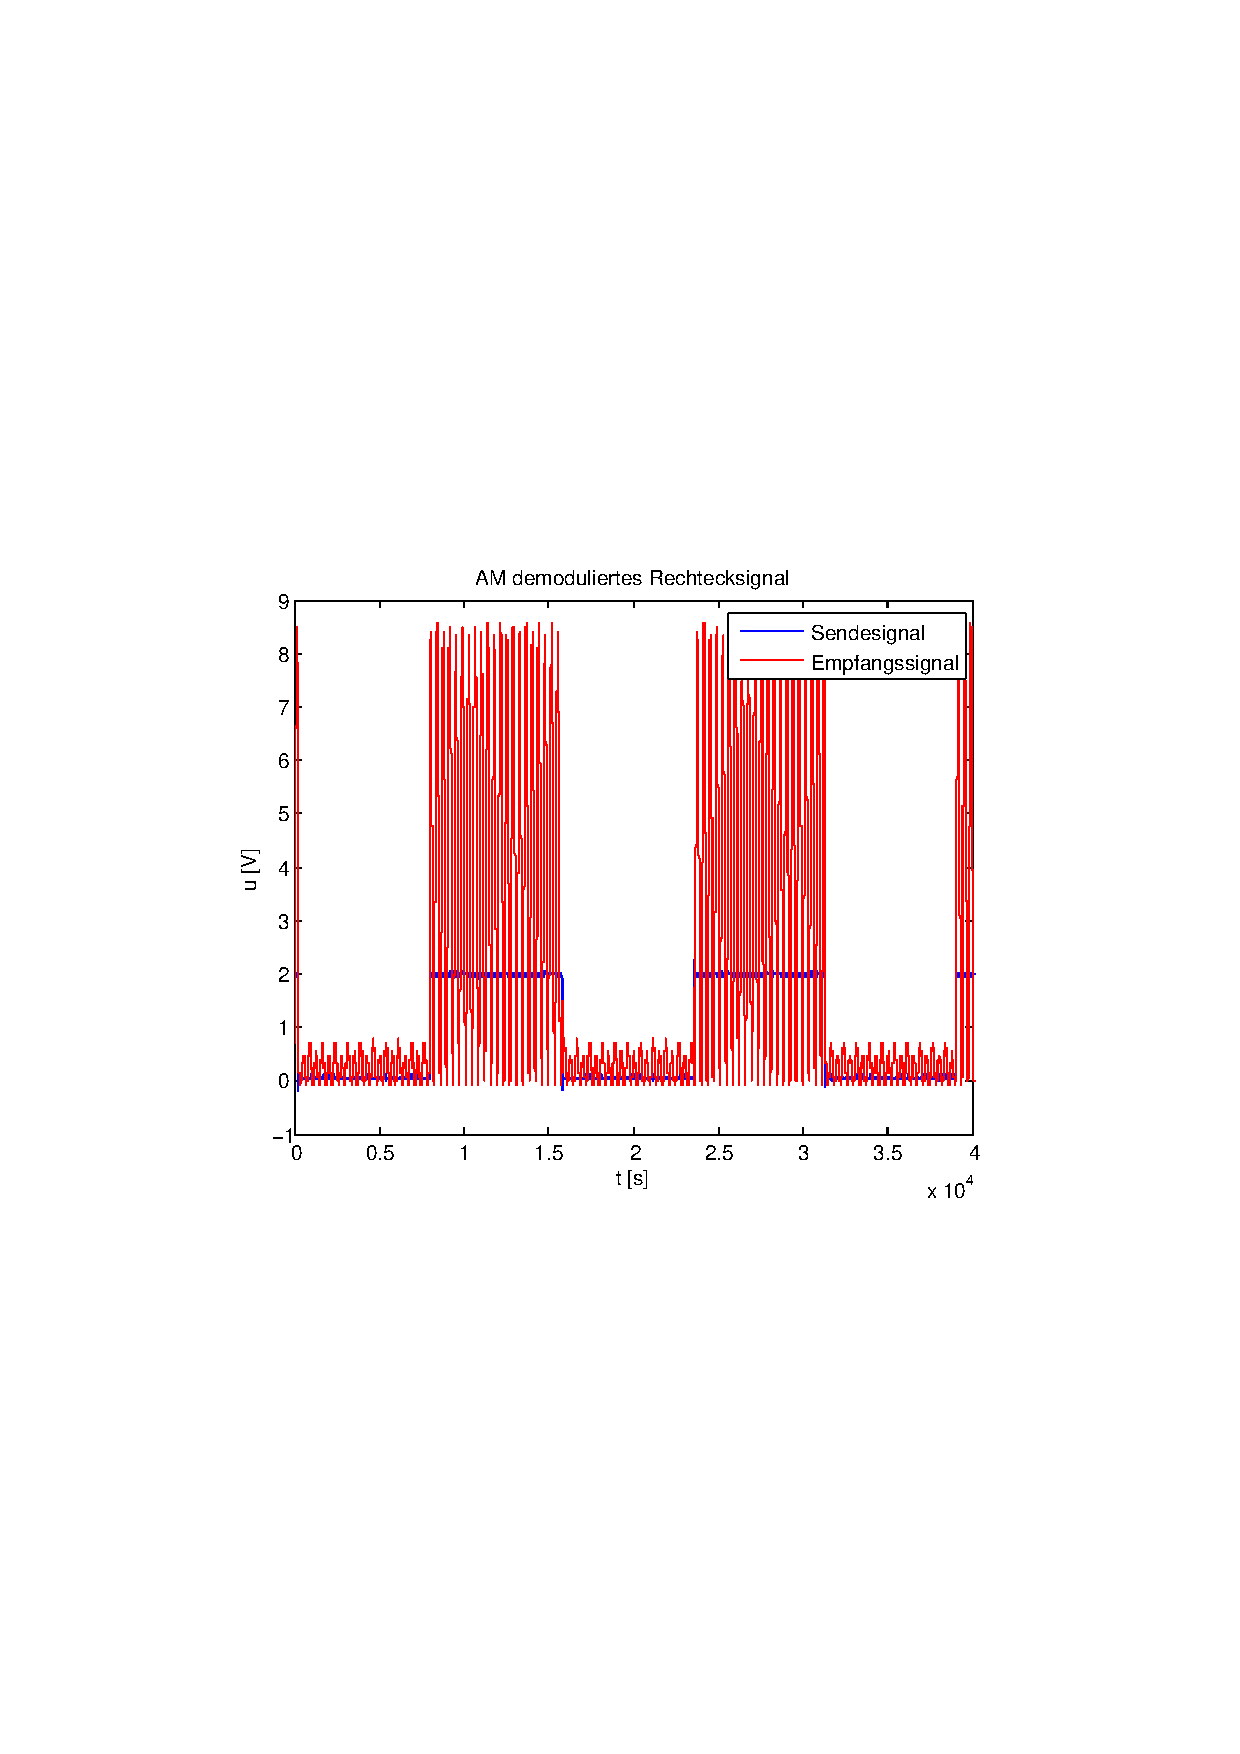
\includegraphics[scale=0.5, trim = 4cm 9.5cm 3.5cm
                        9.5cm,clip]{./Bilder/synchDemod_rechteck}
                            \caption{amplitudendemoduliertes Rechtecksignal}
                    \end{figure}
                    
                    Zunächst ist zu beobachten, dass sich auch hier das Nutzsignal hervorragend
                    erkennen lässt.\\
                    Im Gegensatz zu dem modulierten Signal alterniert das Signal nicht mehr von $-2V$ bis $+2V$ sondern
                    hier von $0V$ bis $+4V$. Dadurch ist das demodulierte Signal dem Eingangssignal ein Schritt
                    ähnlicher geworden. Es unterscheidet sich noch durch einen Verstärkungsfaktor sowie die höheren
                    Frequenzen des Trägersignals von dem originalsignal.\vspace{1em}
                    
                    Der Verstärkungsfaktor von $4$ basiert auf der
                    Multiplikation, die für die Amplitudenmodulation benötigt wird. 
                    Der Maximalwert des Nutzsignals von $2V$ wird zuerst bei der Modulation und später
                    bei der Demodulation mit den $2V$ des Trägersignals multipliziert. Daher der Spitzenwert von $8V$
                    bei dem demodulierten Signal.\\
                    
     			
		\end{quote}
		
		\subsubsection{demodulierte Signale mit Tiefpass}
		\begin{quote}
                    Um die durch die Modulation entstehenden Oberwellen wieder von dem demodulierten Signal zu
                    trennen, wird das Signal noch einmal tiefpassgefiltert. Ein
                    solcher Tiefpass ist schon auf dem Trainingsbrett vorhanden.\\
                    Der TP wurde dabei manuell so eingestellt, bis das Ergebniss ungefähr 
                    den Erwartungen des Sendesignals entsprach. Dabei maßen wir
                    mithilfe des Oszilloskops die jeweiligen Periodendauer von den
                    Empfangssignalen und konnten mit $T_{Periode}$ rückwirkend die
                    Grenzfrequenzen bestimmen. Dabei verwendeten wir den
                    Zusammenhang $f = \frac{1}{T}$. Wichtig dabei war es den in dem
                    TP integrierten Vorfaktor von $100$ zu berücksichtigen, um keine 
                    hundertfache Frequenzen zu erhalten. Es ergab sich für das
                    Sinusempfangssignal eine Periode von $T = 50\mu s$ und die
                    Grenzfrequenz $f = 0.2 kHz$. Für das Dreieckempfangssignal
                    erhielten wir eine Periodendauer von $T = 20\mu s$ und die Grenzfrequenz
                    $f = 0.5 kKz$ sowie eine Periodendauer von $T = 2.5\mu s$ und
                    die Grenzfrequenz $f = 4 kKz$ für das Rechteckempfangssignal.
                    Die Ergebnisse nach der Filterung wurden ebenfalls geplottet und
                    erneut mit dem ursprünglichen Sendesignal verglichen.
                    
                    
       \begin{center}
                \begin{tabular}{ll}
    
                \hspace{-14em}
                    \begin{minipage}{0.6\textwidth}
    
                        \begin{figure}[H]
                            \label{fig:}
                            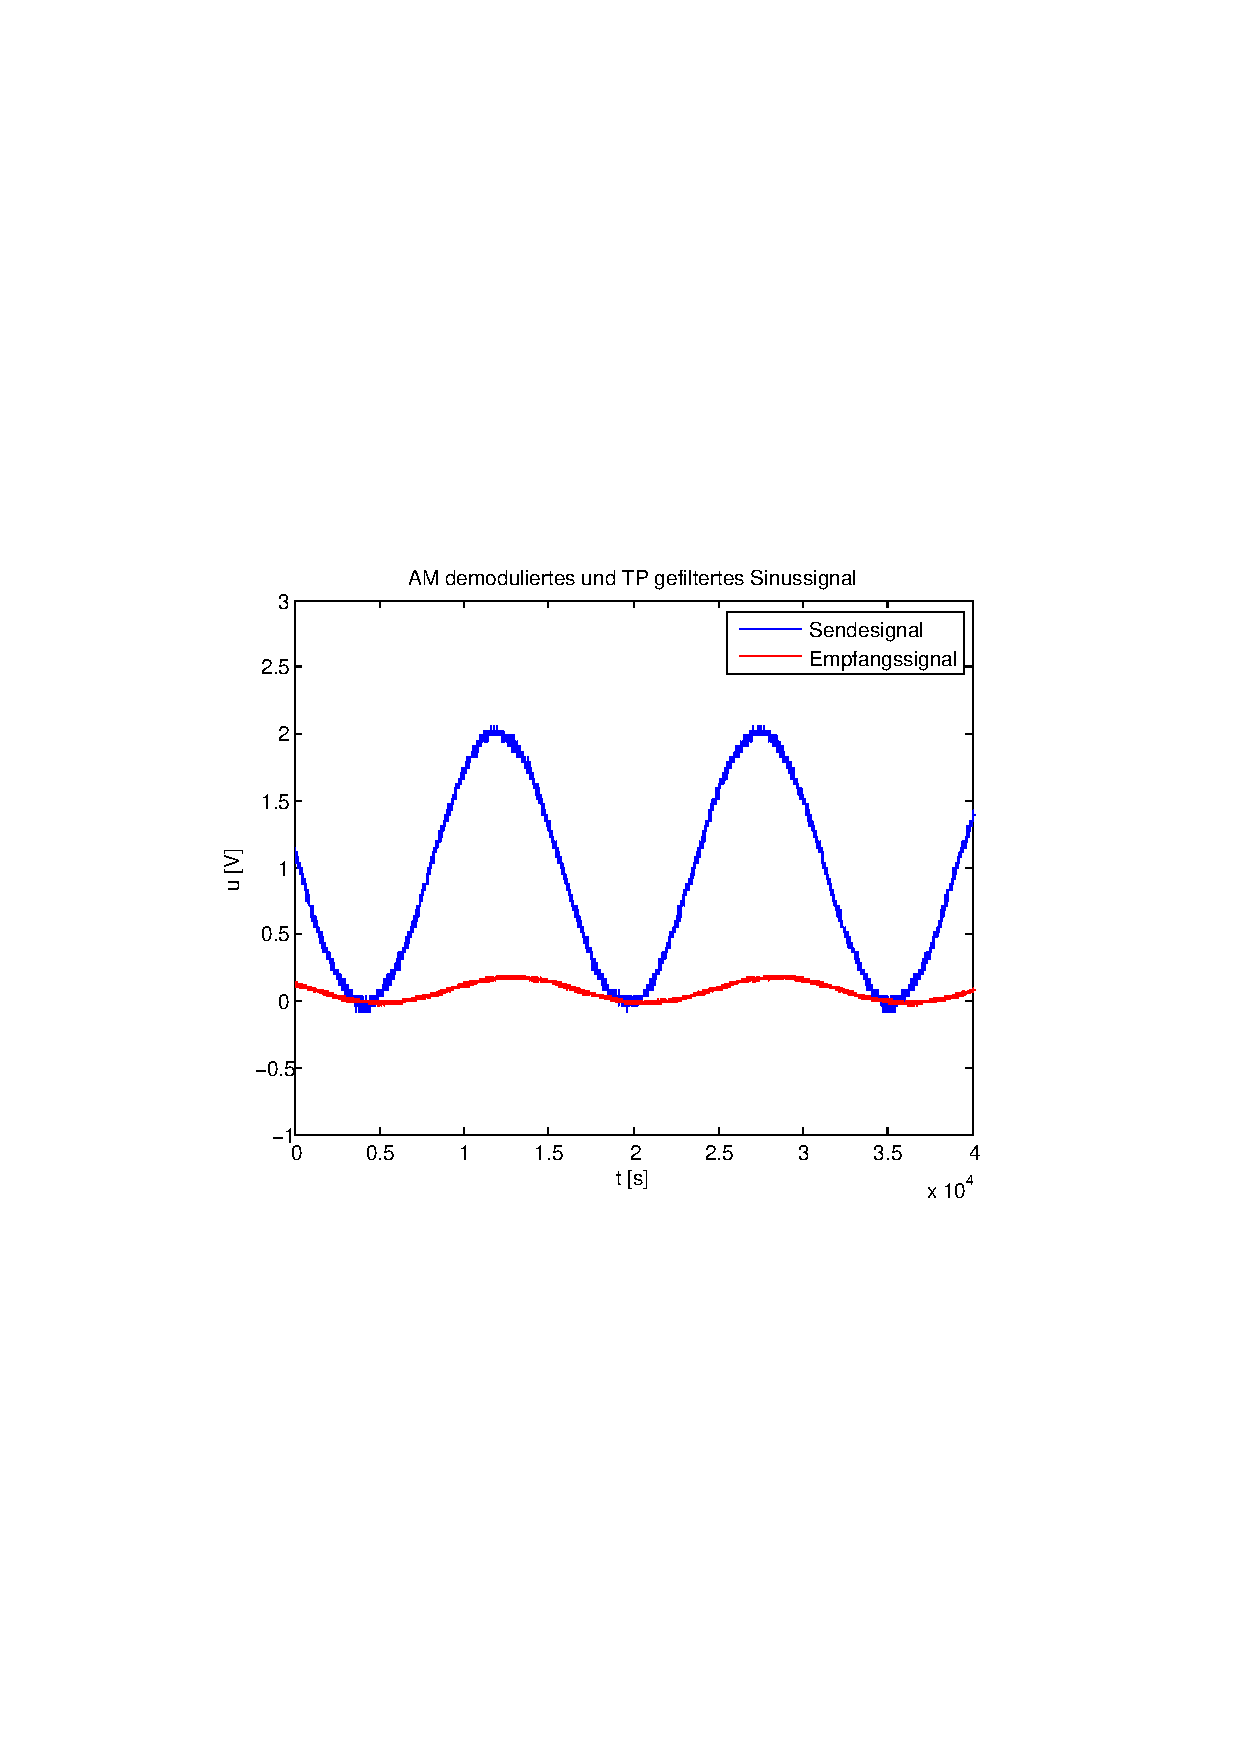
\includegraphics[scale=0.5, trim = 3cm 9cm 3.5cm
                            9.5cm, clip]{./Bilder/synchDemodFilter_sinus} %FIXME
                            % [width=640px, height=474px]
                            \caption{AM-demoduliertes und
                            TP-gefiltertes Sinussignal}
                        \end{figure}
    
                    \end{minipage}
                    \begin{minipage}{0.6\textwidth}
    
                         \begin{figure}[H]
                            \label{fig:}
                            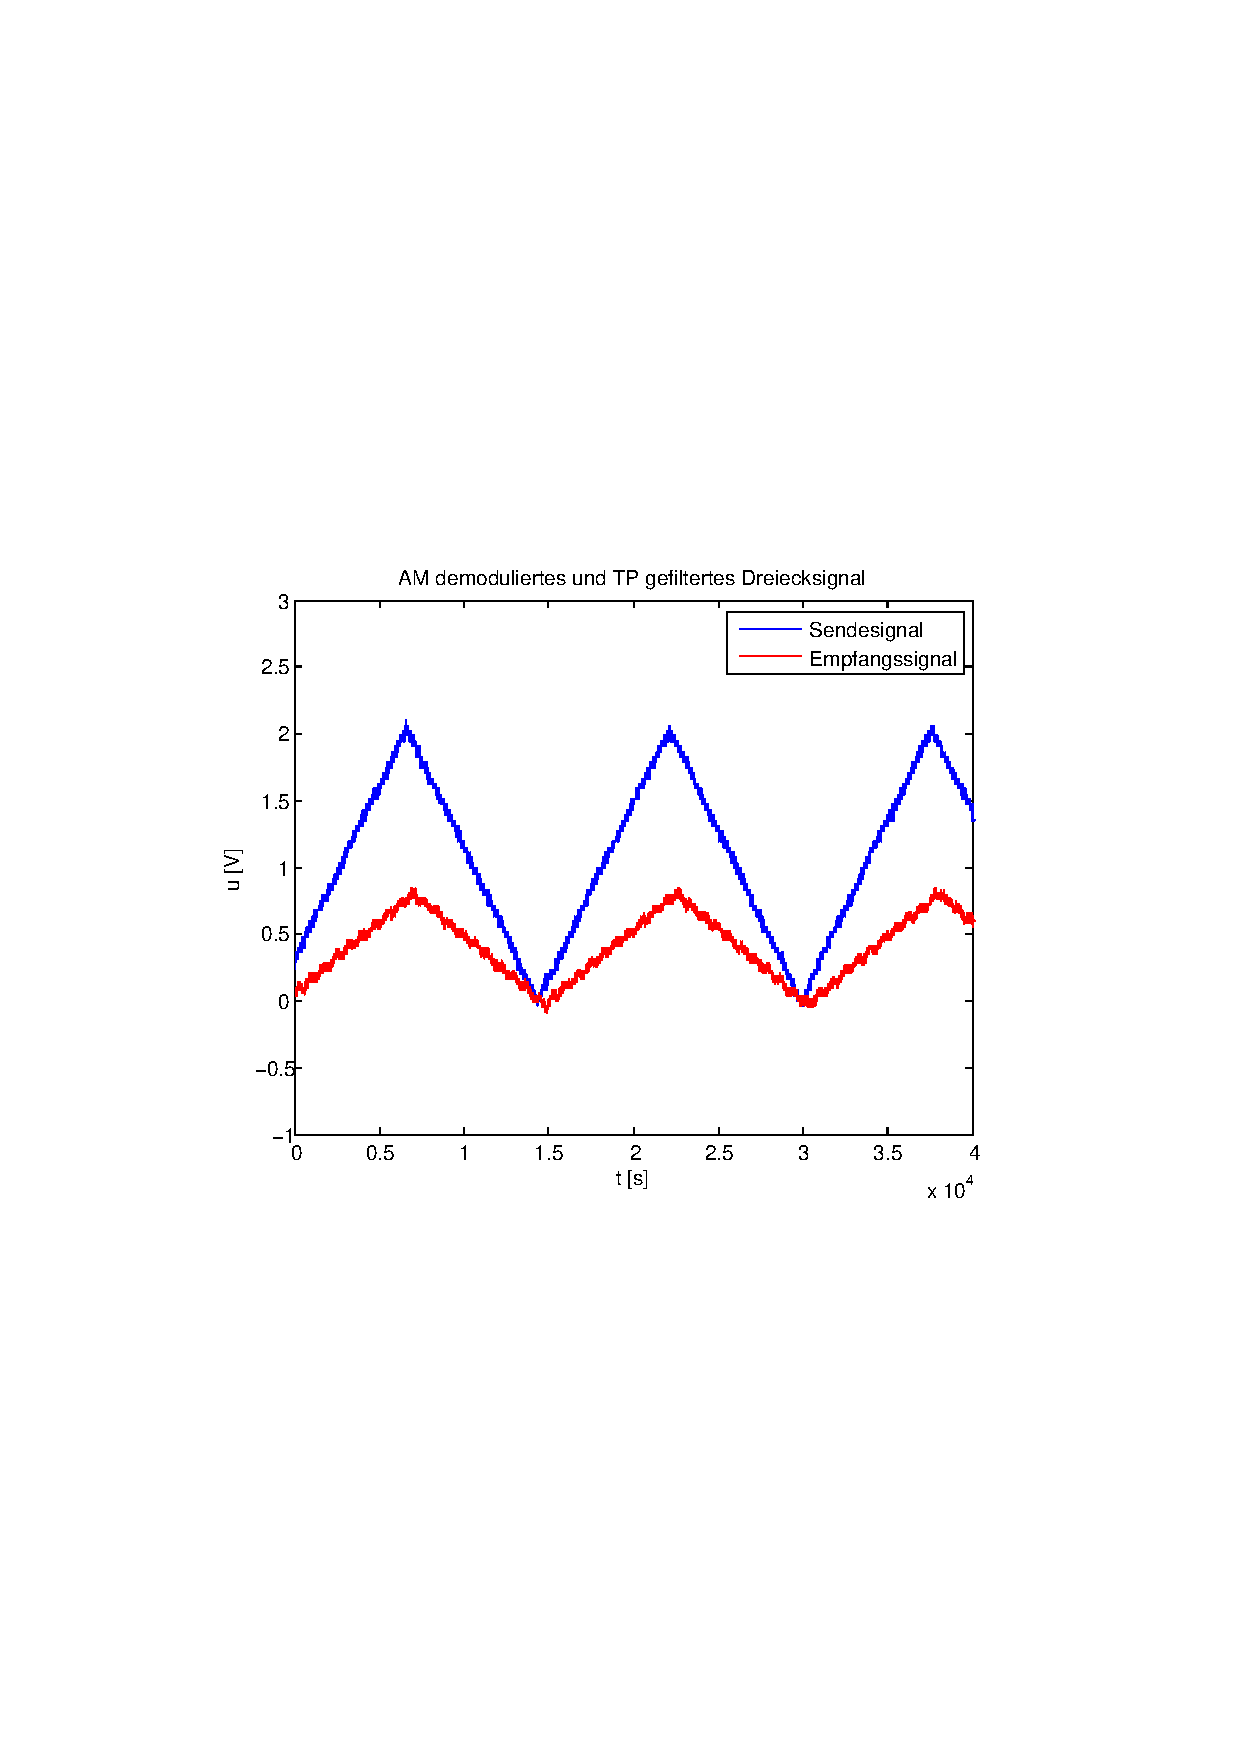
\includegraphics[scale=0.5, trim = 3cm 9cm 3.5cm
                            9.5cm, clip]{./Bilder/synchDemodFilter_dreieck} %FIXME
                            % [width=640px, height=474px]
                            \caption{AM-demoduliertes und
                            TP-gefiltertes Dreiecksignal}
                        \end{figure}
                   \vspace{-1.5em}
    
                    \end{minipage}
    
                \end{tabular}
                \end{center}
                
                 \begin{figure}[H] \centering
                        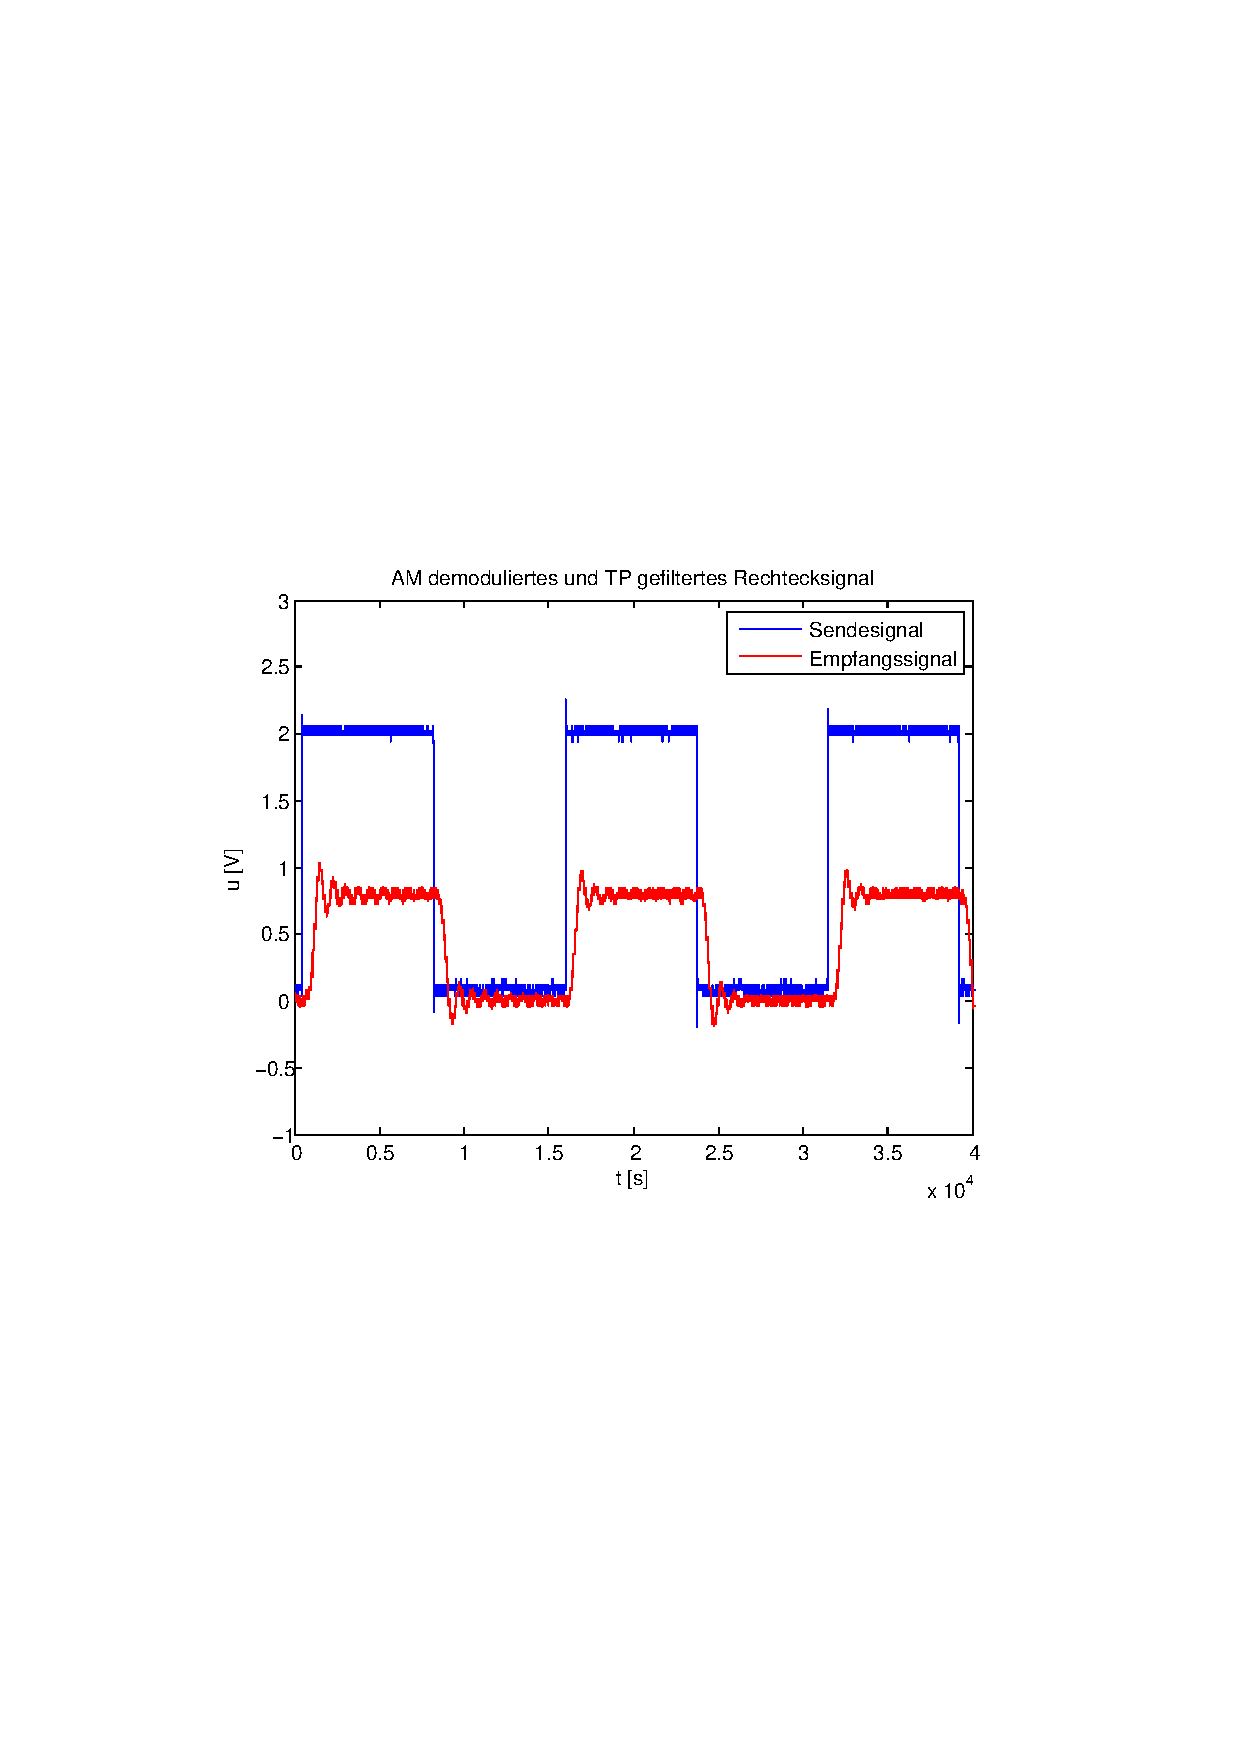
\includegraphics[scale=0.5, trim = 3cm 9cm 3.5cm 9.5cm,
                        clip]{./Bilder/synchDemodFilter_rechteck}
                            \caption{AM-demoduliertes und
                            TP-gefiltertes Rechtecksignal}
                    \end{figure}
    

                    
                    Nach der Tiefpassfilterung erkennt kann aus dem demodulierten Signal glücklicherweise noch das
                    originalsignal erkannt werden. Jedoch müssen wir durch die abschließende Tiefpassfilterung einen
                    erheblichen Qualitätsverlust des Signals hinnehmen. Es ist gut möglich, dass wir mit dem
                    Tiefpassfilter nicht exakt genug gefiltert haben.\\
                    Dass das demodulierte Signal in der Amplitude kleiner ist als das Originalsignal liegt an der
                    Methode der Amplitudenmodulation. Bei jeder multiplikation mit dem Trägersignal wird die Energie des
                    Signals halbiert und um die Trägerfrequenz in positive und negative Richtung verschoben. Das heißt,
                    dass das Ursprungssignal nach zweifacher multuplikation in vier gleichgroße Energiepakete aufgeteilt
                    wurde. Da jedoch zwei dieser vier genau auf der Ursprungsfrequenz landen. Ist ihre Amplitude genau
                    $\frac{1}{2}$ mal so groß wie die Original Amplitude. Mit diesem Wissen können wir das demodulierte
                    Signal einfach verdoppel.\\
                    Bei dem Dreieck- und dem Rechtecksignal klappt diese Methode recht gut.  Das Cosinussignal ist
                    leider immer noch zu klein in der Amplitude. In diesem Fall ist vermutlich wieder die Feinjustierung
                    des Tiefpasses dafür verantwortlich.\\
                    Es lässt sich sagen, dass die Methode der Amplitudenmodulation funktioniert.
                    		
		\end{quote}
    \end{quote}
\end{quote}

%--------------------------------------------------------------------
%--------------------------------------------------------------------            



\section{Frequenzmodulation}
\begin{quote}
    \subsection{Theorie}
    \begin{quote}
        Bei der Frequenzmodulation wird aus dem Nutzsignal mit einer variablen Frequenz und einer variablen Amplitude
        ein moduliertes Signal mit einer festen Amplitude und variabler Frequenz. Die Informationen des Nutzsignals sind
        in diesem Fall in den Frequenzen zu finden. Um dieses umzusetzten wird das modulierte Signal folgendermaßen
        erstellt:
        
        \begin{equation*}
        	\begin{split}
        		u_m (t) = A \cdot cos ( \omega_c t + K_{FM} \cdot \int_{-\infty}^{t} u(\tau) \mathrm d\tau \left)
        	\end{split}
        \end{equation*}
        
        Das Nutzsignal $u(t)$ befindet sich in dieser Formel innerhalb der Cosinusfunktion des Trägersignlas. Daran
        kann man erkennen, dass die Spannung des Nutzsignal einen direkten Einfluss auf die Frequenz des modulierten
        Signals hat.\\
        Dieser Zusammenhang lässt sich  in einer Modulatorkennlinie beschreiben.
        
        \begin{figure}[H]
        \centering
            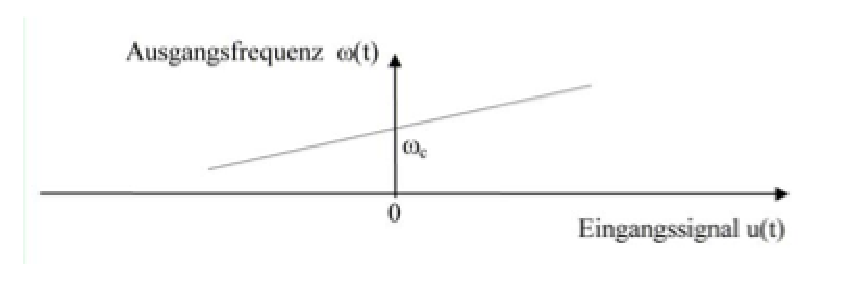
\includegraphics[scale=0.7, trim = 0cm 0cm 0cm 0cm, clip]{./Bilder/Modulatorkennlinie}
                \caption{Modulatorkennlinie}
                \cite{Modulatorkennlinie}
        \end{figure}
    
        Um sich die Auswirkungen einer Frequenzmodulation zu veranschaulichen haben wir einen moduliertes Cosinussignal
        simuliert und geplottet.
        
        \begin{figure}[H]
        \centering
            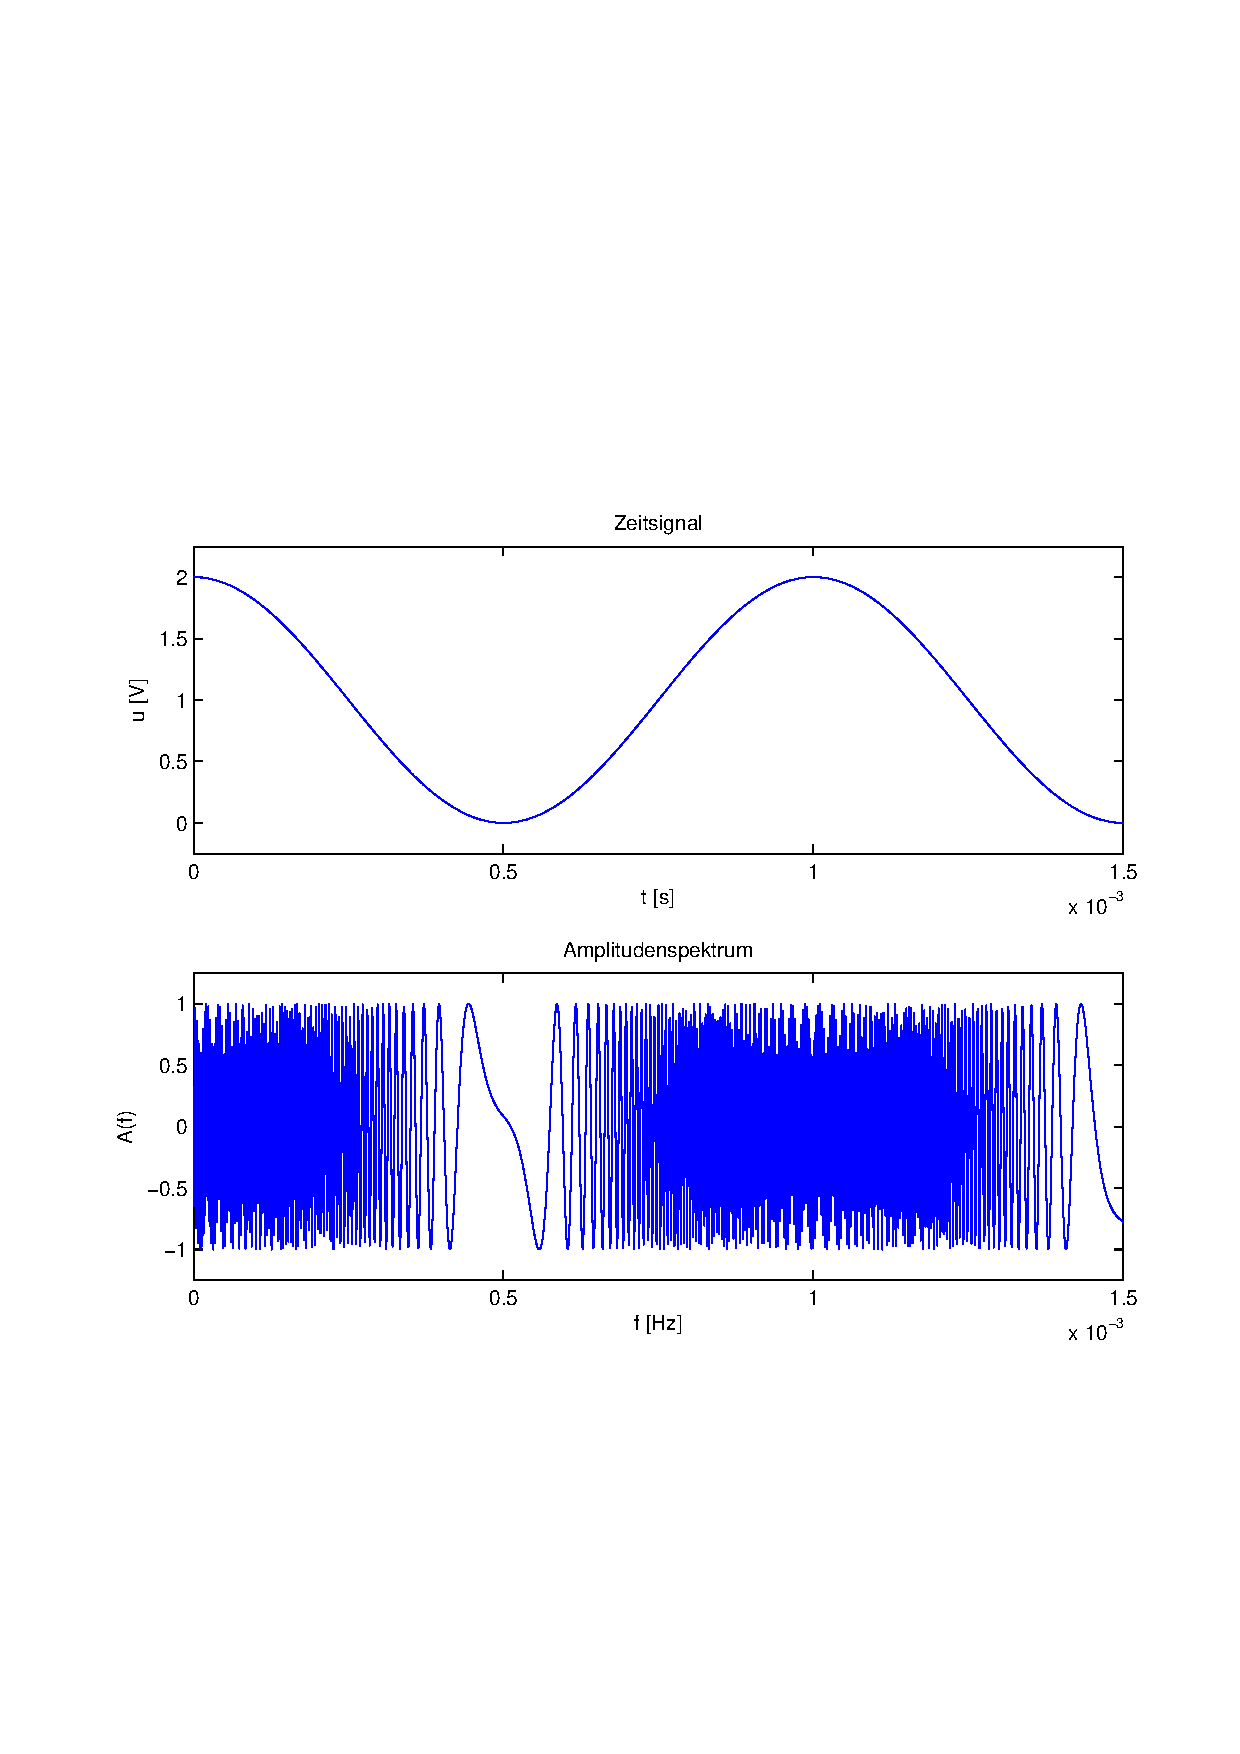
\includegraphics[scale=0.5, trim = 1.5cm 6.5cm 1cm 8cm, clip]{./Bilder/Frequenzmodulation}
                \caption{Frequenzmodulation}
        \end{figure}
        
        In diesem Bild ist sehr schön zu sehen wie die Frequenzen des modulierten Signals von der Amplitude des
        Nutzsignals abhängen. An den Stellen an denen das Nutzsignal ihre maximale Amplitude besitzt, besitzt das
        modulierte Signal gleichzeitig die maximal Frequenz. Ähnliches gilt für die minimale Amplitude bzw. minimale
        Frequenz.\vspace{1em}
        
        An diesem Bild lässt sich auch ein großer Vorteil dieser Art der Modulation erkennen. Das modulierte Signal
        besitzt immer die selbe Amplitude. Würde dieses Signal durch einen Rauschbehafteten Kanal übertragen und dadurch
        mit Rauschen behaftet werden, hätte dieses ausschließlich eine Auswirkung auf die Amplitude und nicht auf die
        Frequenz. Da sich die Information des Nutzsignals jedoch in der Frequenz befindet ist dieses Signal sehr
        Rauschunabhängig.\vspace{1em}
        
        Der Nachteil dieses Verfahrens ist jedoch die Demodulation die komplexer ist als bei der Amplitudendemodulation.
        Eine Variante der Frequenzdemodulation ist, das modulierte Signal zuerst mit einem Bandpass zu filtern. Dadurch
        werden alle durch Rauschen entstandenen Amplituden abgeschnitten. Anschließend wird das Signal durch die
        parallelschaltung zwei weiterer Bandpässe gesendet. Die Ausgangssignale der beiden Bandpasse werden anschließend
        voneinander subtrahiert. Diese Schaltung nennt man Gegentaktdiskriminator. Nach dem Gegentaktdisktiminator ist
        das Nutzsignal noch in Amplitudenmodulierter Form vorhanden. Dieses Signal lässt sich dann so
        Amplitudendemodulieren wie im ersten Abschnitt beschrieben. Zuerst das Signal gleichrichten, anschließend den
        Offset entfernen und abschließend das Signal Tiefpassfiltern.
    
    \end{quote}
    
    \subsection{Vorbereitungsaufgabe}
    \begin{quote}
        Um ein Frequenzmoduliertes Signal zu simulieren, welches wir später mit einem gemessenen Signal zuvergleichen,
        erzeugen wir ein Cosinussignal mit einer Frequenz von $1kHz$ und einer
        Amplitude von $1V$. Anschließend\ldots
        (was fehlt hier noch?)
        Wie schon bei der Amplitudenmodulation  haben wir ein moduliertes Signal erstellt, welches wir später mit einem
        gemessenen Signal vergleichen. Dazu haben wir ein Cosinussignal mit einer Frequenz von
        $1kHz$ und einer Amplitude von $1V$ erzeugt. Anschließend haben wir das Frequenz modulierte Signal mit dem
        vorher erstellen Cosinussignal als Nutzsignal erzeugt.\\
        Dieses modulierte Signal haben wir abschließend geplottet.
    \end{quote}
    
    \subsection{Durchführung}
    \begin{quote}
        \subsubsection{Signalerzeugung}
        \begin{quote}
        Als Nutzsignal für die Frequenzmodulation wird ein $3 kHz$-Sinus mit
        einer $1 V$-Amplitude verwendet. Die einfache Modulation verwirklichten
        wir anhand des VCO-Moduls. Dabei wurde der Schalter in der Mitte auf
        die Position LOW gesetzt (das Trägersignal kann damit eine
        Nutzsignalfrequenz zwischen $1 kHz$ und $17 kHz$ annehmbar modulieren),
        der FREQ-Controller auf die mittlere Position gestellt und GAIN auf
        $\approx \frac{2}{3}$ des Maximalwerts gedreht.\\
        Als nächstes wurde das Spektrum des FM-Signals untersucht und die
        Trägerfrequenz $f_c$ sowie die Proportionalitätskonstante $K_{FM}$
        bestimmt. Für die Proportionalitätskonstante gilt folgende Formel:
        
        \begin{equation*}
    	\begin{split}
    		K_{FM} &= \frac{2 \pi \Delta f_{max}}{A_u}\\
			\Delta f_{max} &\approx \frac{1}{2} (\frac{1}{T_{min}} - \frac{1}{T_{max}})    		
    	\end{split}
    	\end{equation*}
    	
   		$T_{min}$ und $T_{max}$ bezeichnen dabei die zeitlich kürzeste und längste
   		Periodendauer des Sinussignals.\\
   		Für einen späteren Vergleich wird auch das Spektrum des FM-Signals
   		untersucht, bei der die Nutzfrequenz $f_u = 1 kHz$ und die Nutzamplitude
   		$A_u = 1 V$ beträgt.\\
   		Zusätzlich wurden noch die Nutzsignale mit den Amplituden $0.5 V\, 1 V$ und
   		$2 V$ mit den Frequenzen $50 Hz\, 100 Hz$ und $200 Hz$ frequenzmoduliert
   		und die Spektren des Ausgangs von dem VCO-Modul miteinander verglichen. 
        \end{quote}
        
        \subsubsection{FM-Demodulation}
        \begin{quote}
        Für die folgende FM-Demodulation wurde zunächst die Einstellungen des VCO-Moduls verändert. Der Schalter wurde
        auf HIGH gelegt (nun kann das Trägersignal Nutzfrequenzen zwischen $60 kHz$ und $140 kHz$ modulieren), sowie der
        Trägerfrequenz-Drehknopf auf die Hälfte und der GAIN-Drehknopf auf $70 \%$ eingestellt. Das neu FM-modulierte
        Sinussignal, mit ursprünglich $100 Hz$-Frequenz und $1 V$-Amplitude, wurde dann auf den Eingang des
        Comparator-Moduls gelegt und mit einer Referenzspannung von $0 V$ verglichen.\\
        
        Die FM-Demodulation erfolgt in diesem Praktikum durch eine FM-PFM-Umwandlung (PFM = Pulsfrequenzmodulation).
        Dabei wandelt der Comparator das analoge Signal in ein Standard-Digitalsignal um. Dieses besteht aus einer
        polaren Rechteckfolge, welche dadurch entsteht, dass der Comparator jedesmal, wenn das Analogsignal (in diesem
        Fall der von uns verwendete Sinus) das Referenzsignal übersteigt, einen positiven Ausgangssignalpegel ausgibt.
        Wird das Analogsignal kleiner als die Referenzspannung wird der Ausgangssignalpegel negativ. Dieses digitale
        Signal wird in den Twin Pulse Generator (TPG) geführt, der aus jeder steigenden Flanke ein Rechteckimpuls
        verwirklicht. Dafür werden die Regler DELAY und WIDTH auf ihr Minimum gedreht. Durch diese Rechteckimpule werden
        quasi die Nulldurchgänge gezählt. Und in diesen Nulldurchgängen steckt weiterhin die Information über die
        Frequenz des Signals. Die Pulse des entstandenen Rechtecksignals werden abschließend wieder zu einem
        kontinuierlichen Signalpegel umgewandelt, indem sie durch einen Tiefpass (TP) geführt werden.\\
        
        In der Auswertung vergleichen wir zusätzlich das Sinusquellsignal mit dem Comparator-Ausgang, das
        Sinusquellsignal mit dem Twin Pulse Generator-Ausgang und den Comparator-Ausgang mit dem Twin Pulse
        Generator-Ausgang.
         
        \end{quote}
        
    \end{quote}
    
    \subsection{Auswertung}
    \begin{quote}
    	
    	\subsubsection{Signalerzeugung und Modulation}
    	\begin{quote}
    	
        Nach der Frequenzmodulation des Sinusnutzsignals mit der Frequenz 
        $3 kHz$ und der Amplitude $1 V$ erhielten wir folgendes Zeitsignal.
    	
             \begin{figure}[H] \centering
                   
                    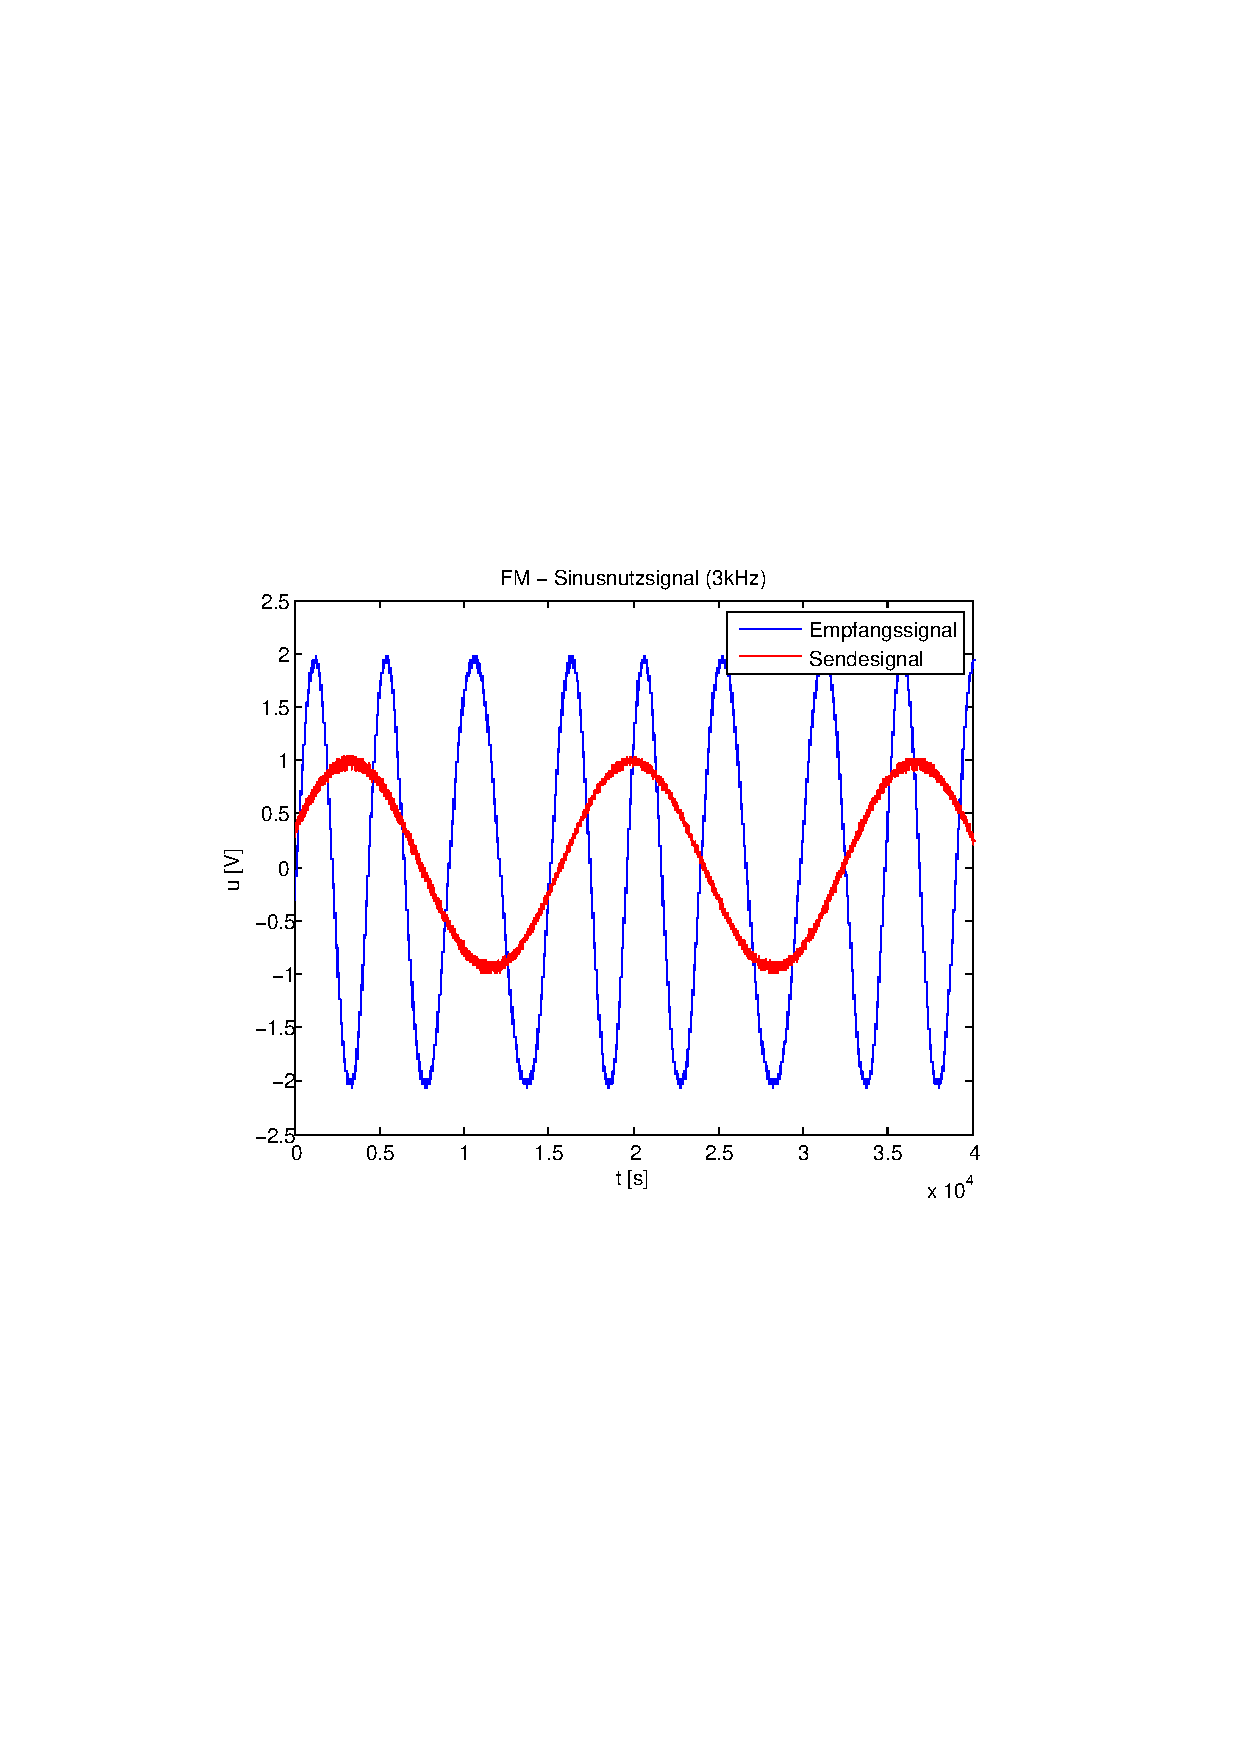
\includegraphics[scale=0.5, trim = 3cm 8.5cm 3.5cm 8.5cm,
                    clip]{./Bilder/fm_sinus(3kHz)}
                        \caption{frequenzmoduliertes Sinusnutzsignal (3kHz)}
                \end{figure}
        
        Das Verhältnis dieser beiden Signale wurde mit dem Oszilloskop genauer
        untersucht um die Proportionalitätskonstante berechnen zu können. Dafür
        zoomten wir einmal in einen passenden Bereich, wo die Amplitude des
        Nutzsignals ihr Maximum hatte und einmal in einen passenden Bereich, wo die
        Amplitude des Nutzsignals ihr Minimum hatte.
        
                    \begin{figure}[H]
                        \label{fig:}                    
                        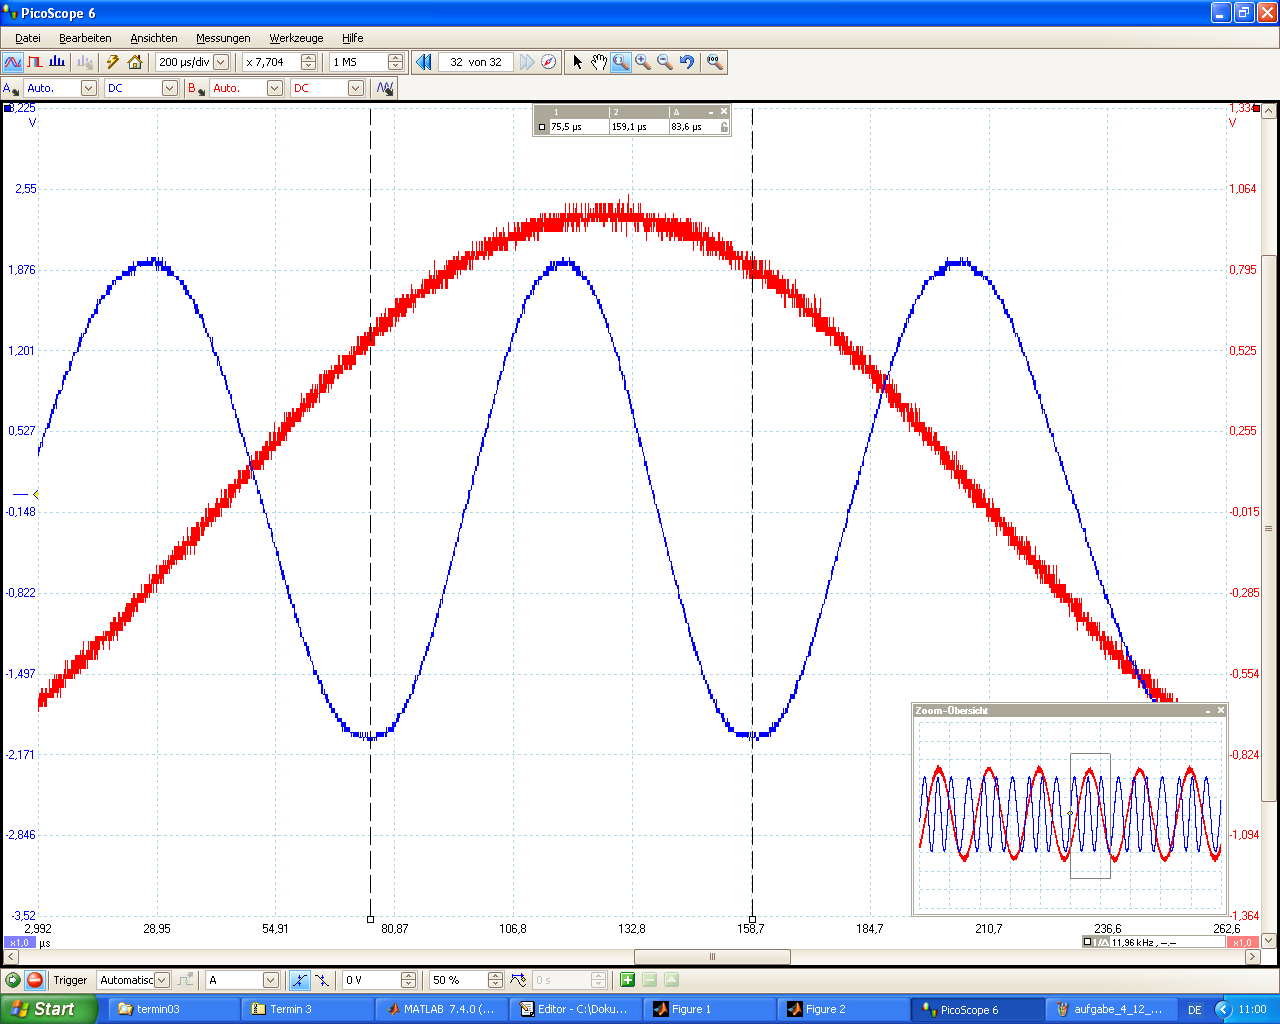
\includegraphics[scale=0.2, trim = 0cm 1.5cm 0cm
                        2.5cm, clip]{./Bilder/aufgabe_4_12_sinus_high-ampl}
                        %FIXME [width=640px, height=474px]
                        \caption{max Amplitude des Nutzsignals zur
                        Periodendauerbestimmung (Tmin) des FM-Empfangssignals}
                    \end{figure}

                     \begin{figure}[H]
                        \label{fig:}
                        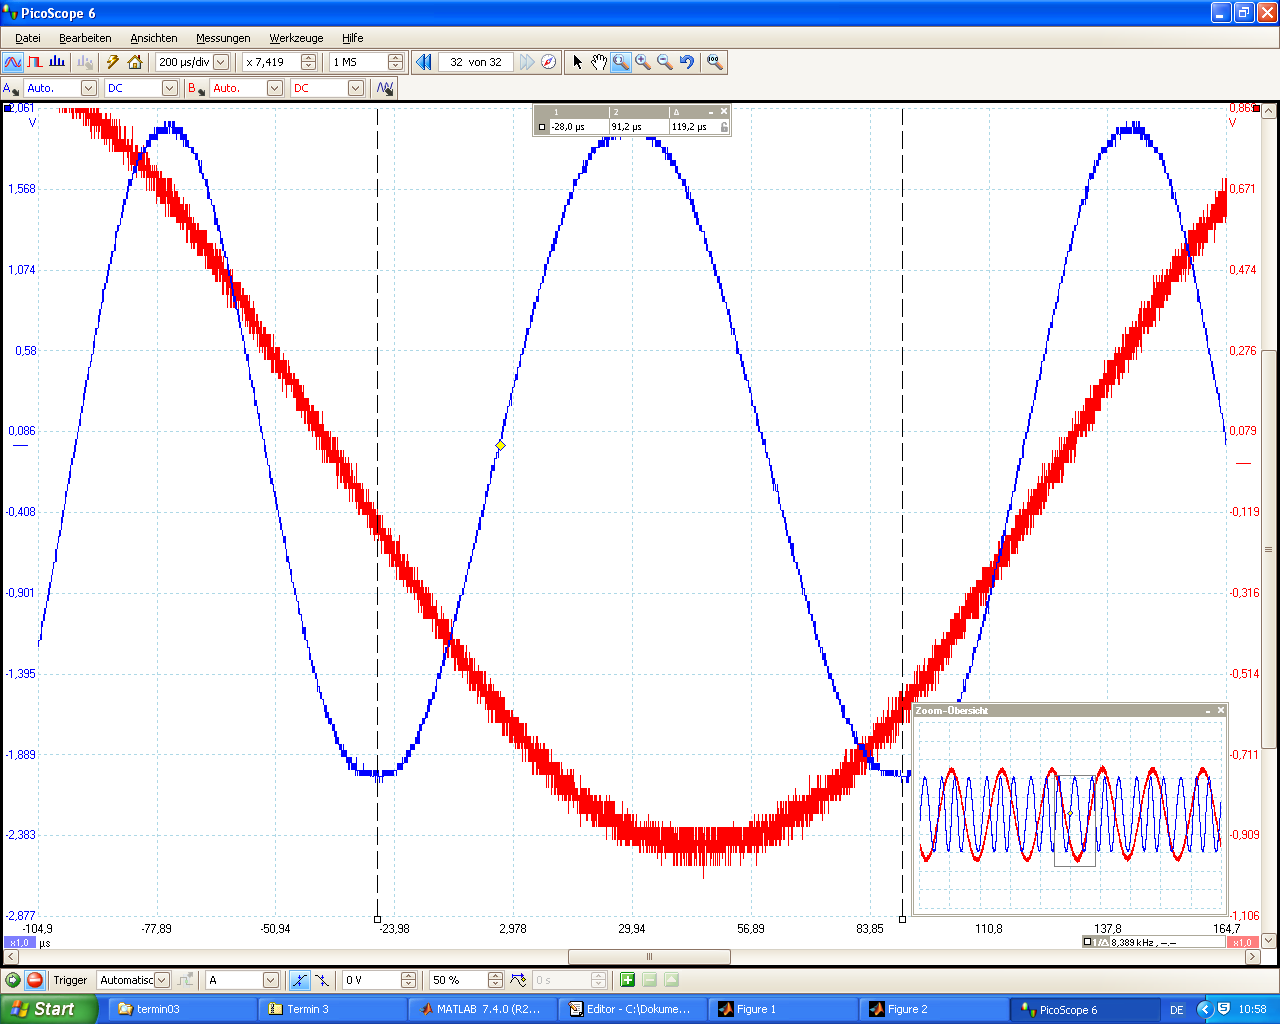
\includegraphics[scale=0.2, trim = 0cm 1.5cm 0cm
                        2.5cm, clip]{./Bilder/aufgabe_4_12_sinus_low-ampl}
                        %FIXME [width=640px, height=474px]
                        \caption{min Amplitude des Nutzsignals zur
                        Periodendauerbestimmung (Tmax) des FM-Empfangssignals}
                    \end{figure}
                   \vspace{-1.5em}
        
        Bei der ersten Messung erhielten wir eine $T_{min}$ von ungefähr 
        $84\mu s$, bei der zweiten Messung waren es für $T_{max}$ ungefähr 
        $120\mu s$. Mit diesen Werten können wir zunächst das $\Delta f_{max}$
        berechnen, womit sich dann auch das $K_{FM}$ (mit $A_u = 1V$) berechnen
        lässt.
        
      \begin{equation*}
       \begin{split}
		\Delta f_{max} &\approx \frac{1}{2} (\frac{1}{84\mu s} - \frac{1}{120\mu s})\\
					   &\approx 1.786 kHz \\
		\\		
	    K_{FM} &= \frac{2 \pi \cdot 1.786 kHz}{1 V}\\
	    	   &= 11221.768    		
       \end{split}
     \end{equation*}
     
        
        Somit beträgt unser Proportionalitätsfaktor $K_{FM} = 11221.768$.\\
        
        Für die Berechnung der Trägerfrequenz wird folgendes getan\ldots 
       \TODO{müssen wir auf jeden Fall noch ergänzen} 
        
        Um einen Vergleich anstellen zu können, wurde auch das Spektrum des
        Sinussignals mit $1 kHz$ Frequenz aufgenommen. Die Ergebnisse folgen
        hier:
        
                \begin{center}
            \begin{tabular}{ll}

            \hspace{-10em}
                \begin{minipage}{0.6\textwidth}

                    \begin{figure}[H]
                        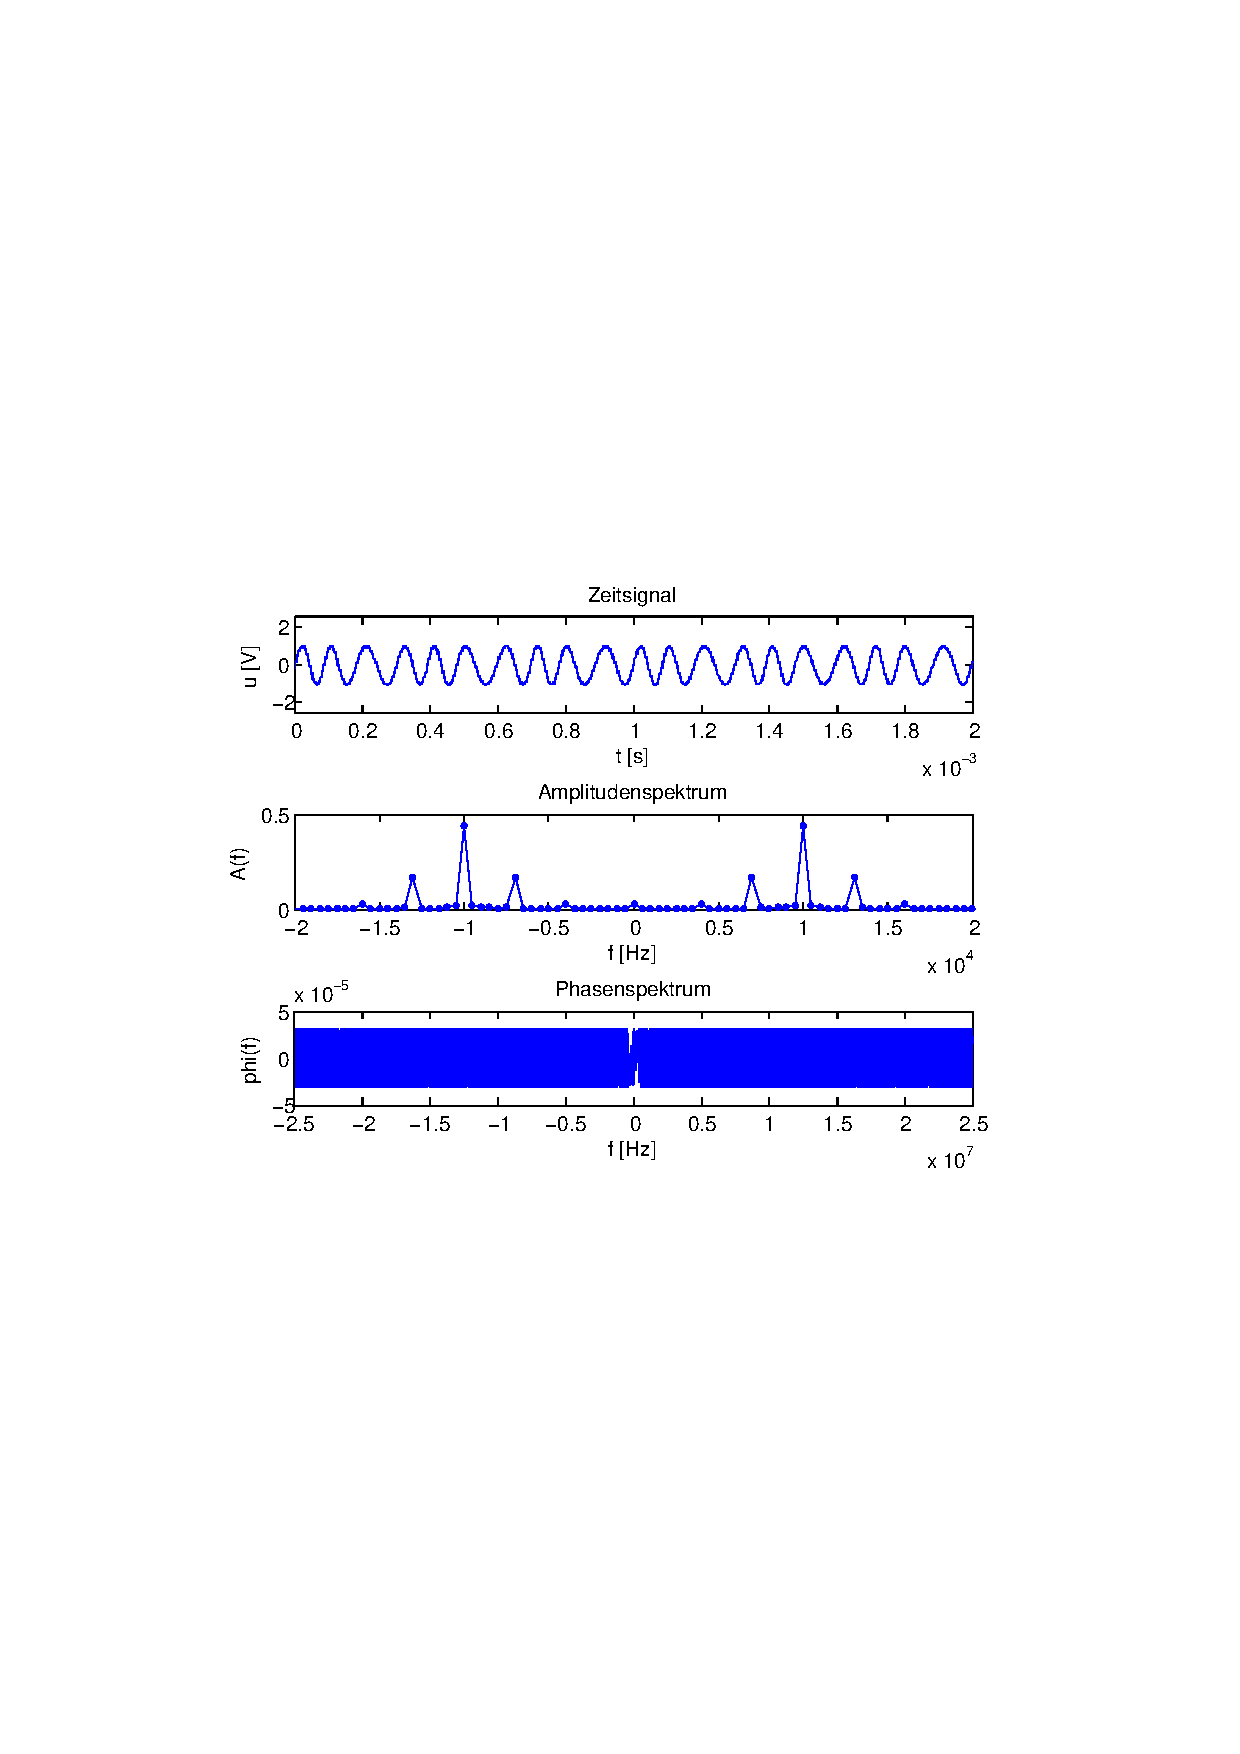
\includegraphics[scale=0.5, trim = 4cm 9.5cm 3.5cm
                        9.5cm, clip]{./Bilder/spektrum_sin3kHz}
                        %FIXME [width=640px, height=474px]
               
                        \caption{Spektrum für das Nutzsignal (3kHz, 1V)}
                    \end{figure}

                \end{minipage}
                \begin{minipage}{0.6\textwidth}

                     \begin{figure}[H]
                        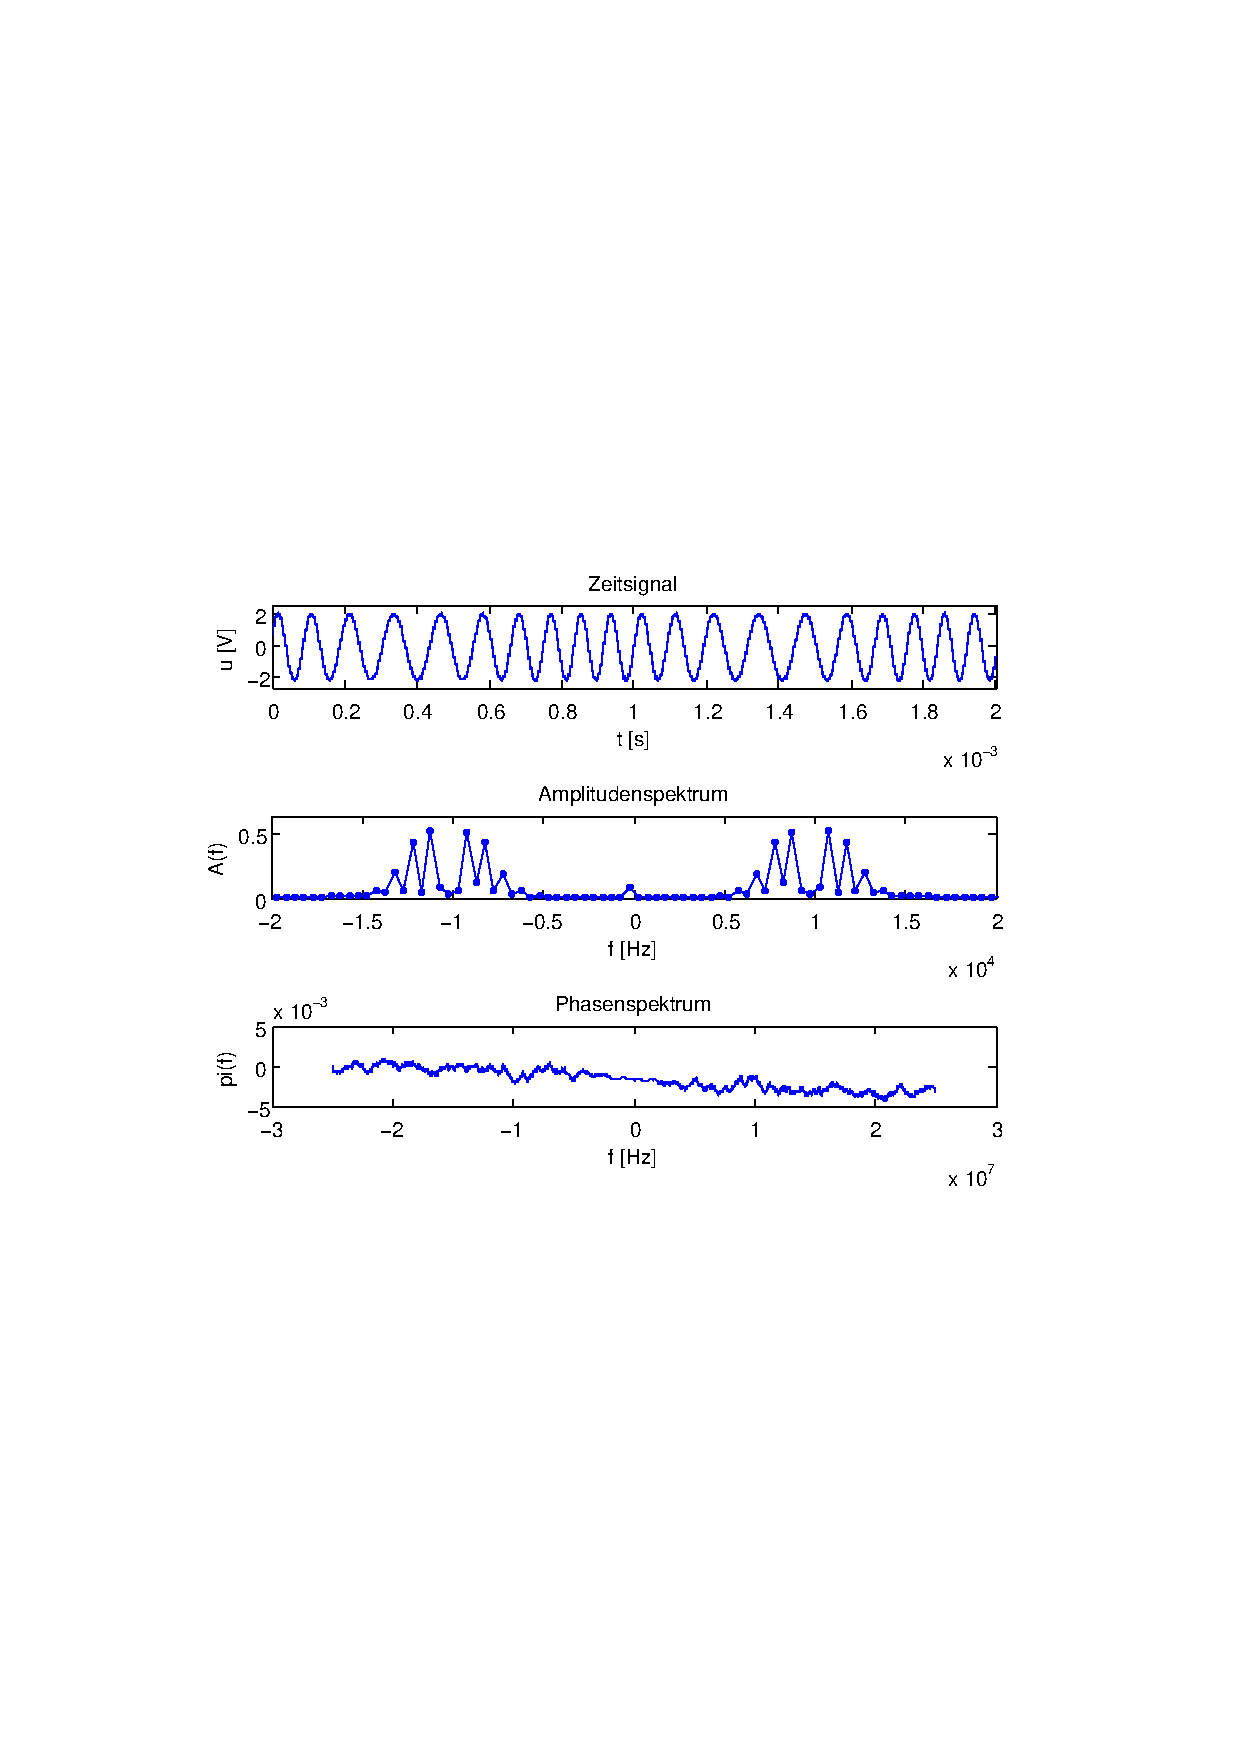
\includegraphics[scale=0.5, trim = 4cm 9.5cm 3.5cm
                        9.5cm, clip]{./Bilder/spektrum_sin1kHz}
                        %FIXME [width=640px, height=474px]
                        \caption{Spektrum für das Nutzsignal (1kHz, 1V)}
                    \end{figure}
               \vspace{-1.5em}

                \end{minipage}

            \end{tabular}
            \end{center}
        
        An den Spektren kann man sehen \ldots \\
        \TODO{noch zu ergänzen}
        
        Um die Auswirkung von Frequenz und Amplitude genauer untersuchen zu
        können, führten wir noch weitere Sinusnutzsignal-Messungen durch mit den
        jeweiligen Amplituden $0.5V, 1V$ und $2V$, sowie den Frequenzen $50Hz,
        100Hz$ und $200Hz$. Folgende Spektren sind daraus entstanden:
        
               \begin{center}
            \begin{tabular}{ll}

            \hspace{-10em}
                \begin{minipage}{0.6\textwidth}

                    \begin{figure}[H]
                        \label{fig:}
                        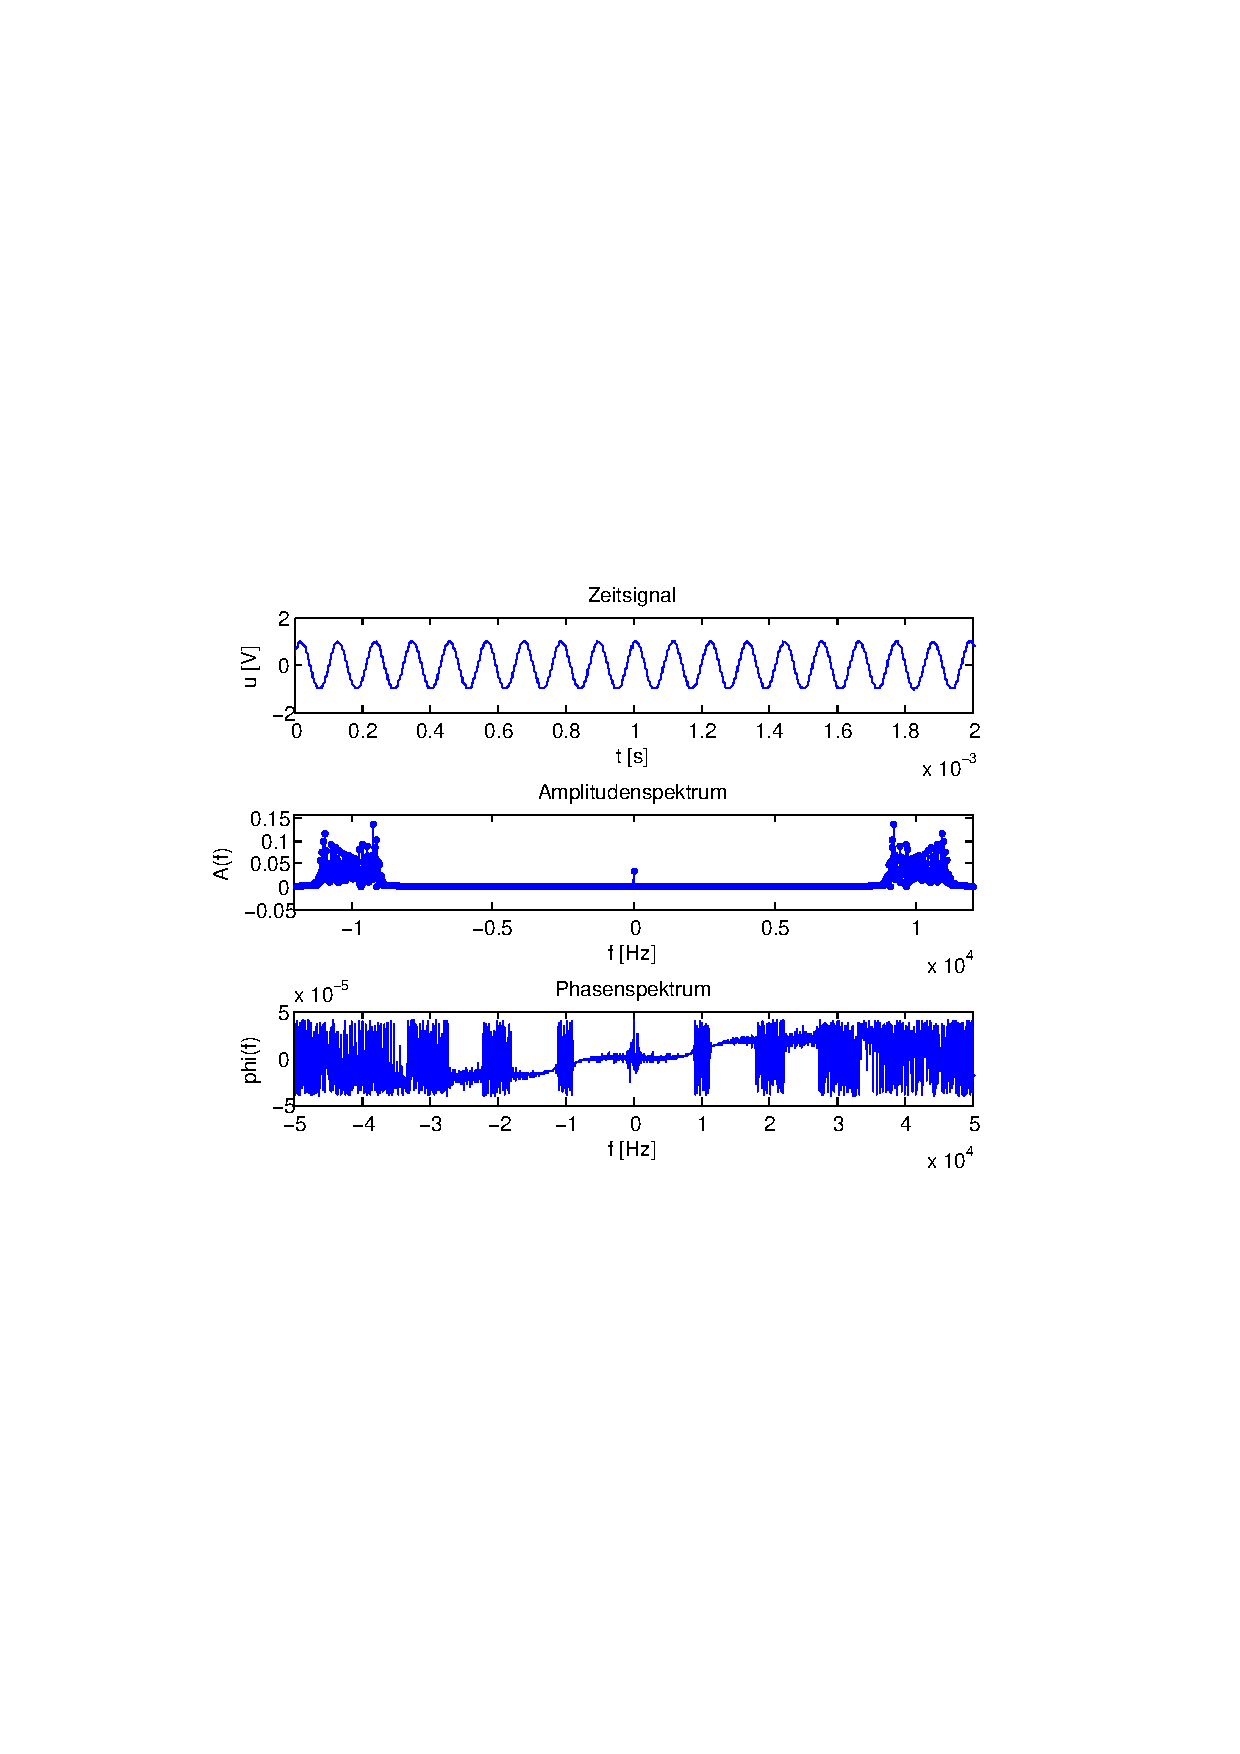
\includegraphics[scale=0.5, trim = 4cm 9.5cm 3.5cm
                        9.5cm, clip]{./Bilder/sin_a05_f50}
                        %FIXME [width=640px, height=474px]
                        \caption{Spektrum für Sinusnutzsignal (0.5V, 50Hz)}
                    \end{figure}

                \end{minipage}
                \begin{minipage}{0.6\textwidth}

                     \begin{figure}[H]
                        \label{fig:}
                        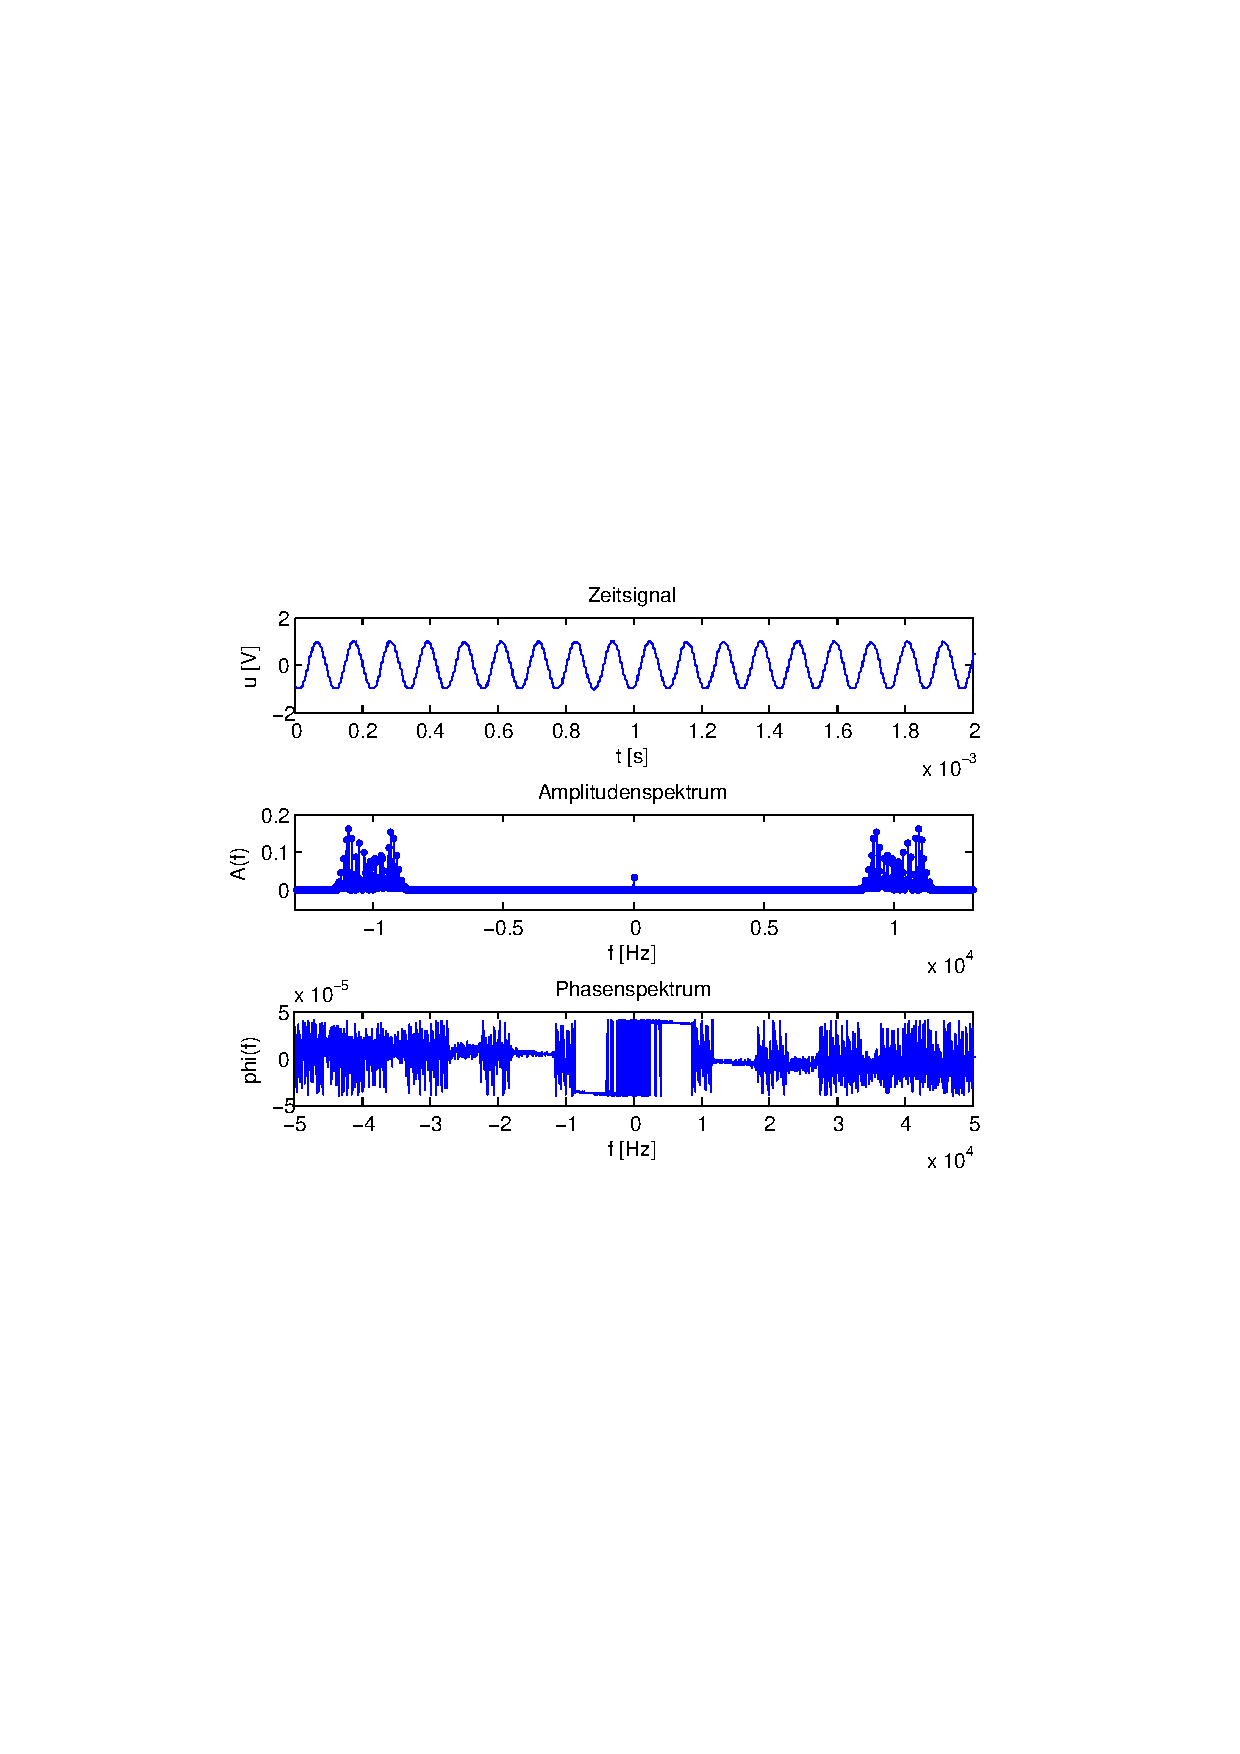
\includegraphics[scale=0.5, trim = 4cm 9.5cm 3.5cm
                        9.5cm, clip]{./Bilder/sin_a05_f100}
                        %FIXME [width=640px, height=474px]
                        \caption{Spektrum für Sinusnutzsignal (0.5V, 100Hz)}
                    \end{figure}
               \vspace{-1.5em}

                \end{minipage}

            \end{tabular}
            \end{center}
            
            %Erste Reihe mit 2 Bildern
            
                   \begin{center}
            \begin{tabular}{ll}

            \hspace{-10em}
                \begin{minipage}{0.6\textwidth}

                    \begin{figure}[H]
                        \label{fig:}
                        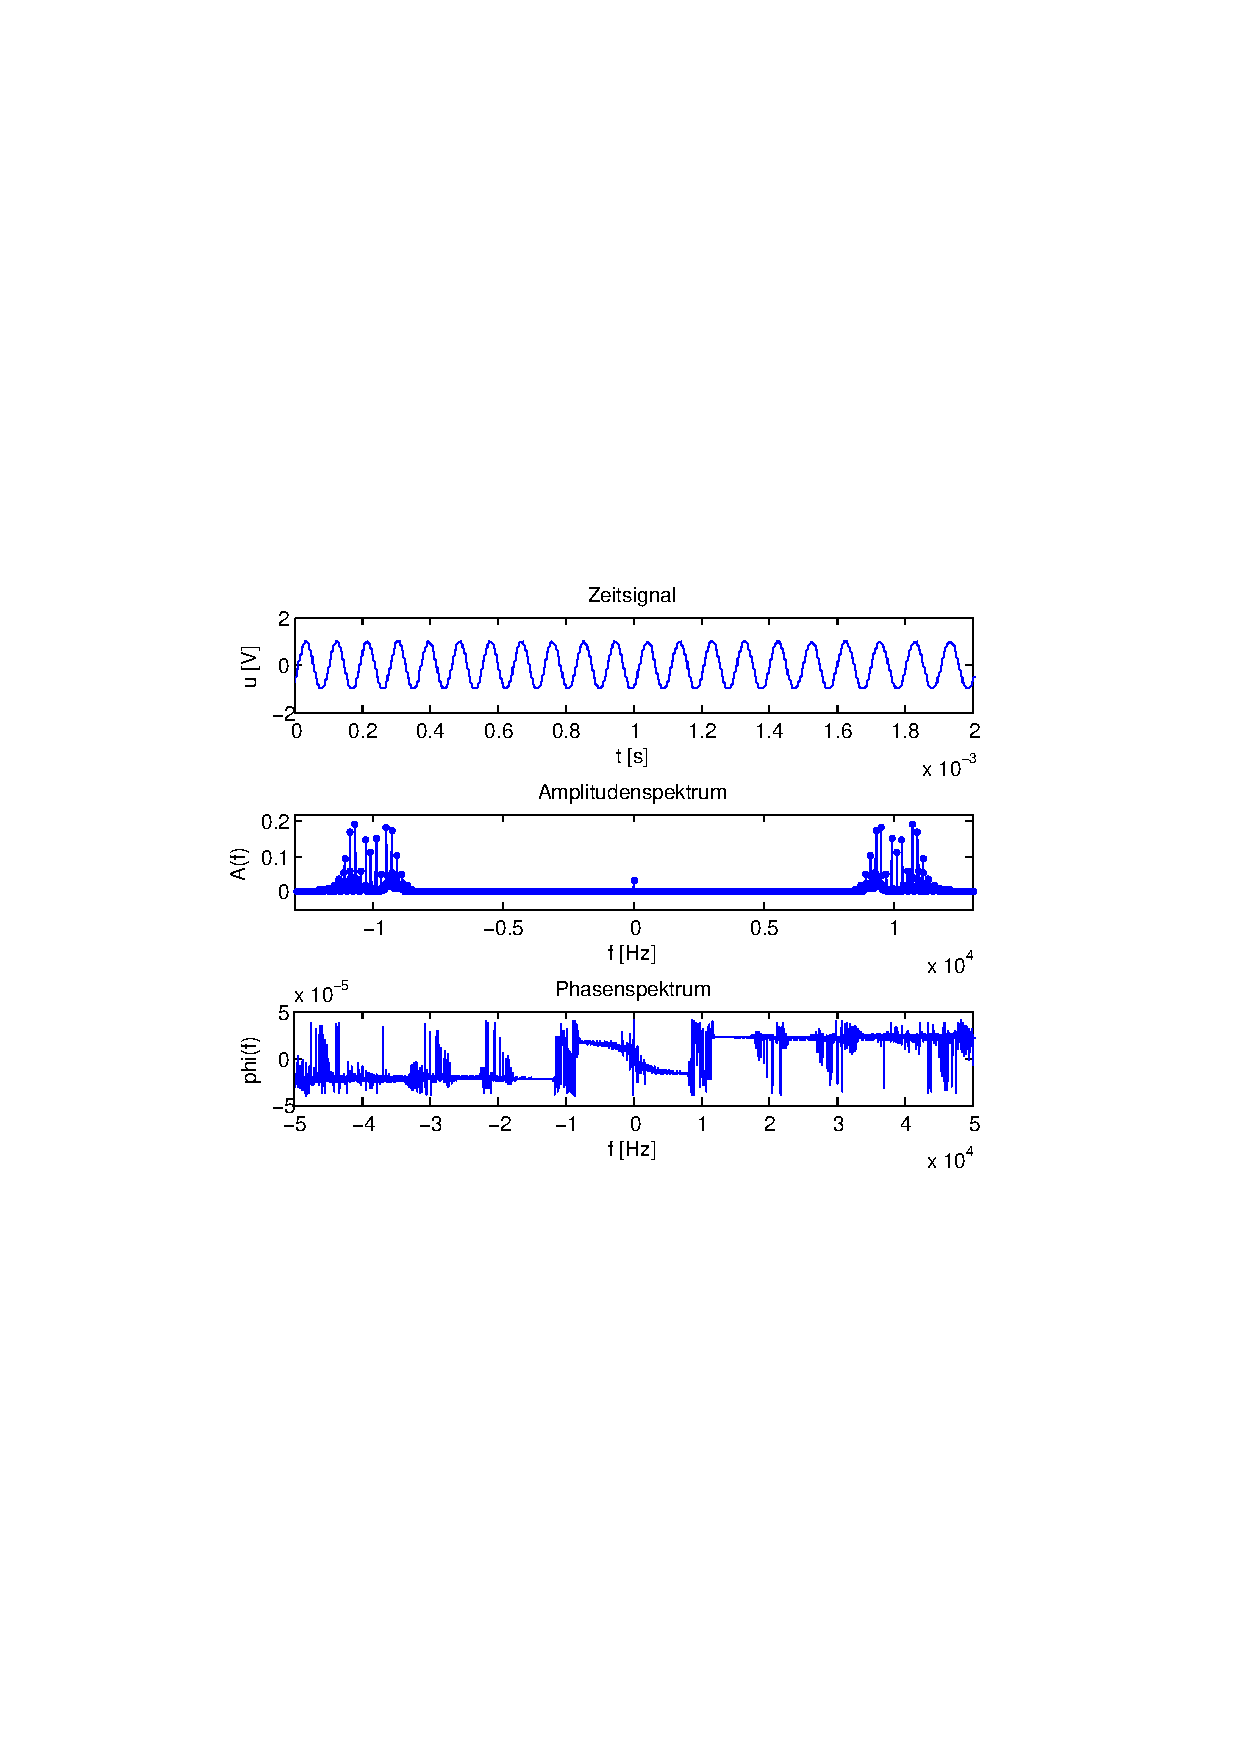
\includegraphics[scale=0.5, trim = 4cm 9.5cm 3.5cm
                        9.5cm, clip]{./Bilder/sin_a05_f200}
                        %FIXME [width=640px, height=474px]
                        \caption{Spektrum für moduliertes Sinusnutzsignal (0.5V,
                        200Hz)}
                    \end{figure}

                \end{minipage}
                \begin{minipage}{0.6\textwidth}

                     \begin{figure}[H]
                        \label{fig:}
                        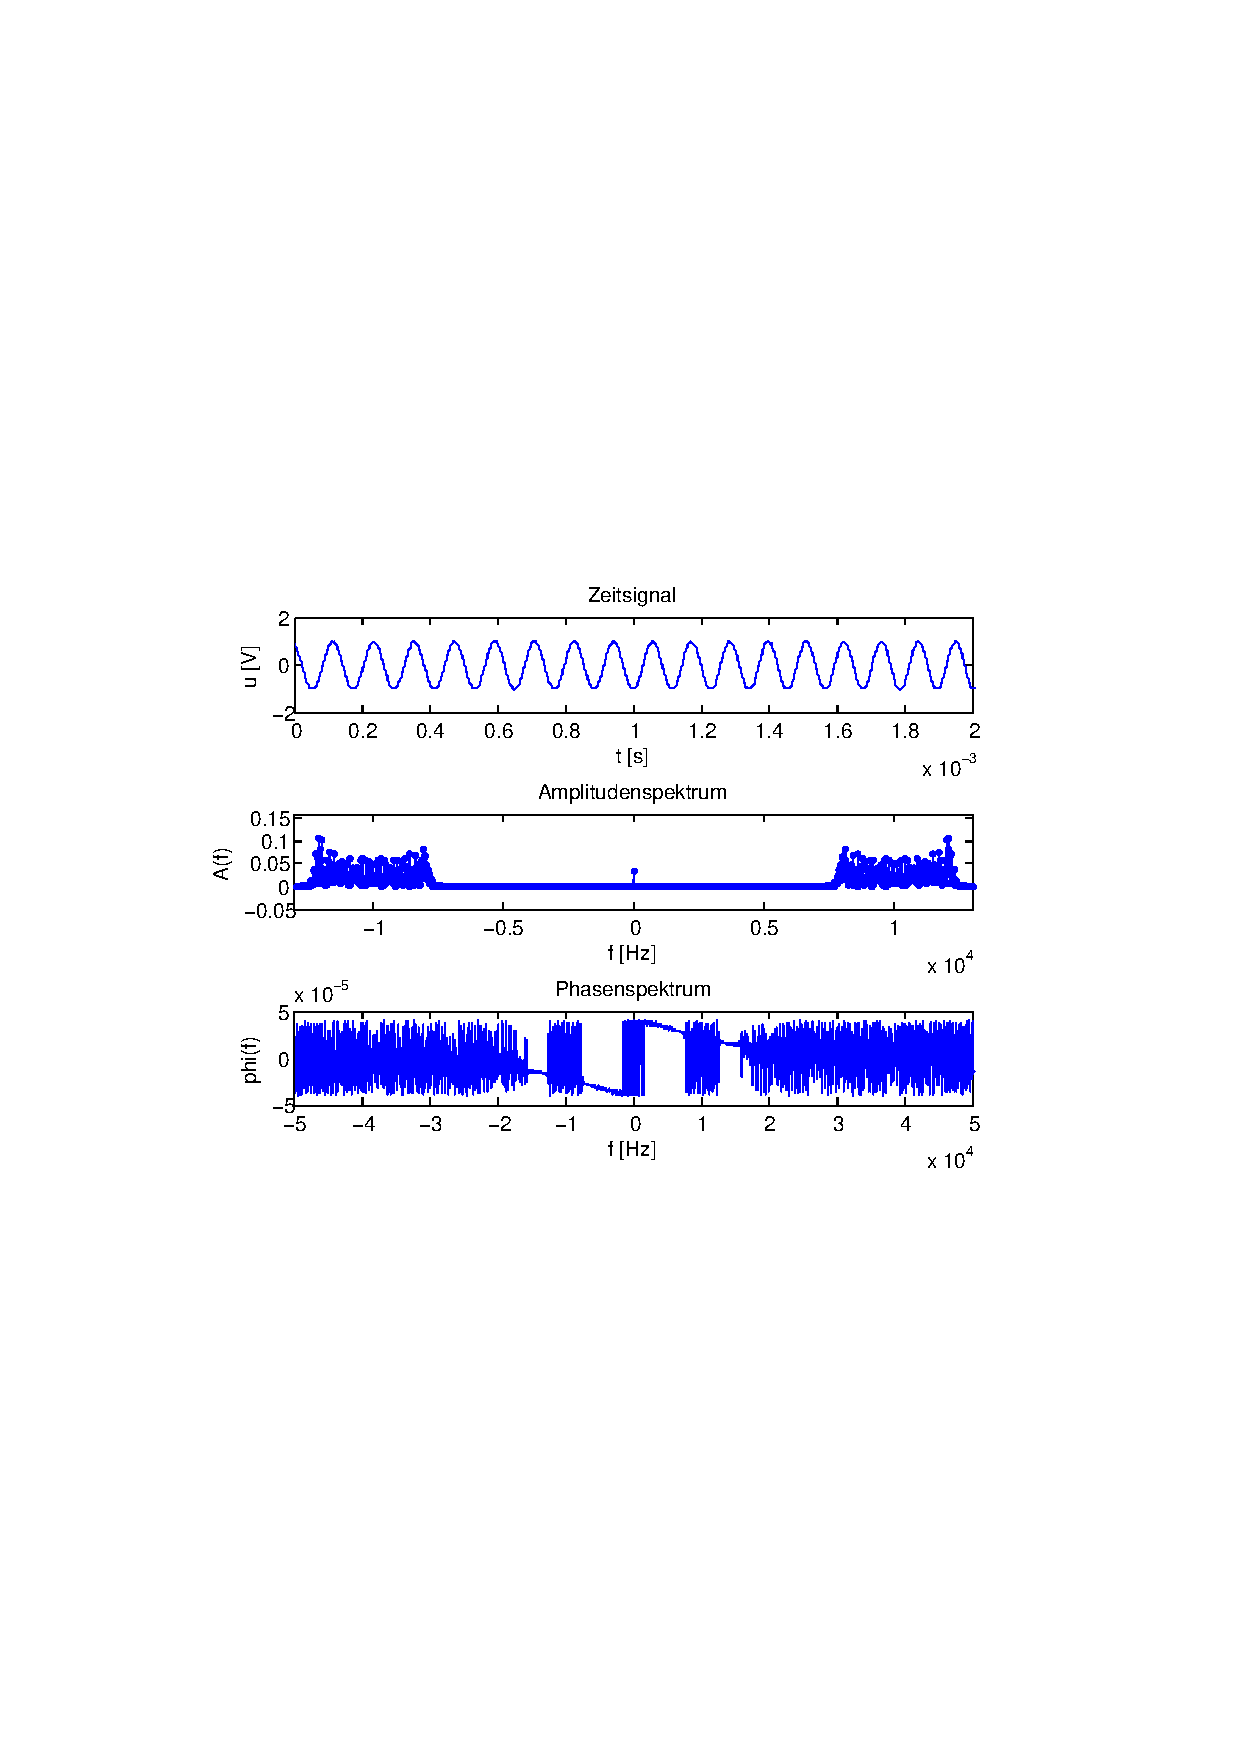
\includegraphics[scale=0.5, trim = 4cm 9.5cm 3.5cm
                        9.5cm, clip]{./Bilder/sin_a1_f50}
                        %FIXME [width=640px, height=474px]
                        \caption{Spektrum für moduliertes Sinusnutzsignal (1V,
                        50Hz)}
                    \end{figure}
               \vspace{-1.5em}

                \end{minipage}

            \end{tabular}
            \end{center}
        	
        	%Zweite Reihe mit 2 Bildern
        	   
        	       \begin{center}
            \begin{tabular}{ll}

            \hspace{-10em}
                \begin{minipage}{0.6\textwidth}

                    \begin{figure}[H]
                        \label{fig:}
                        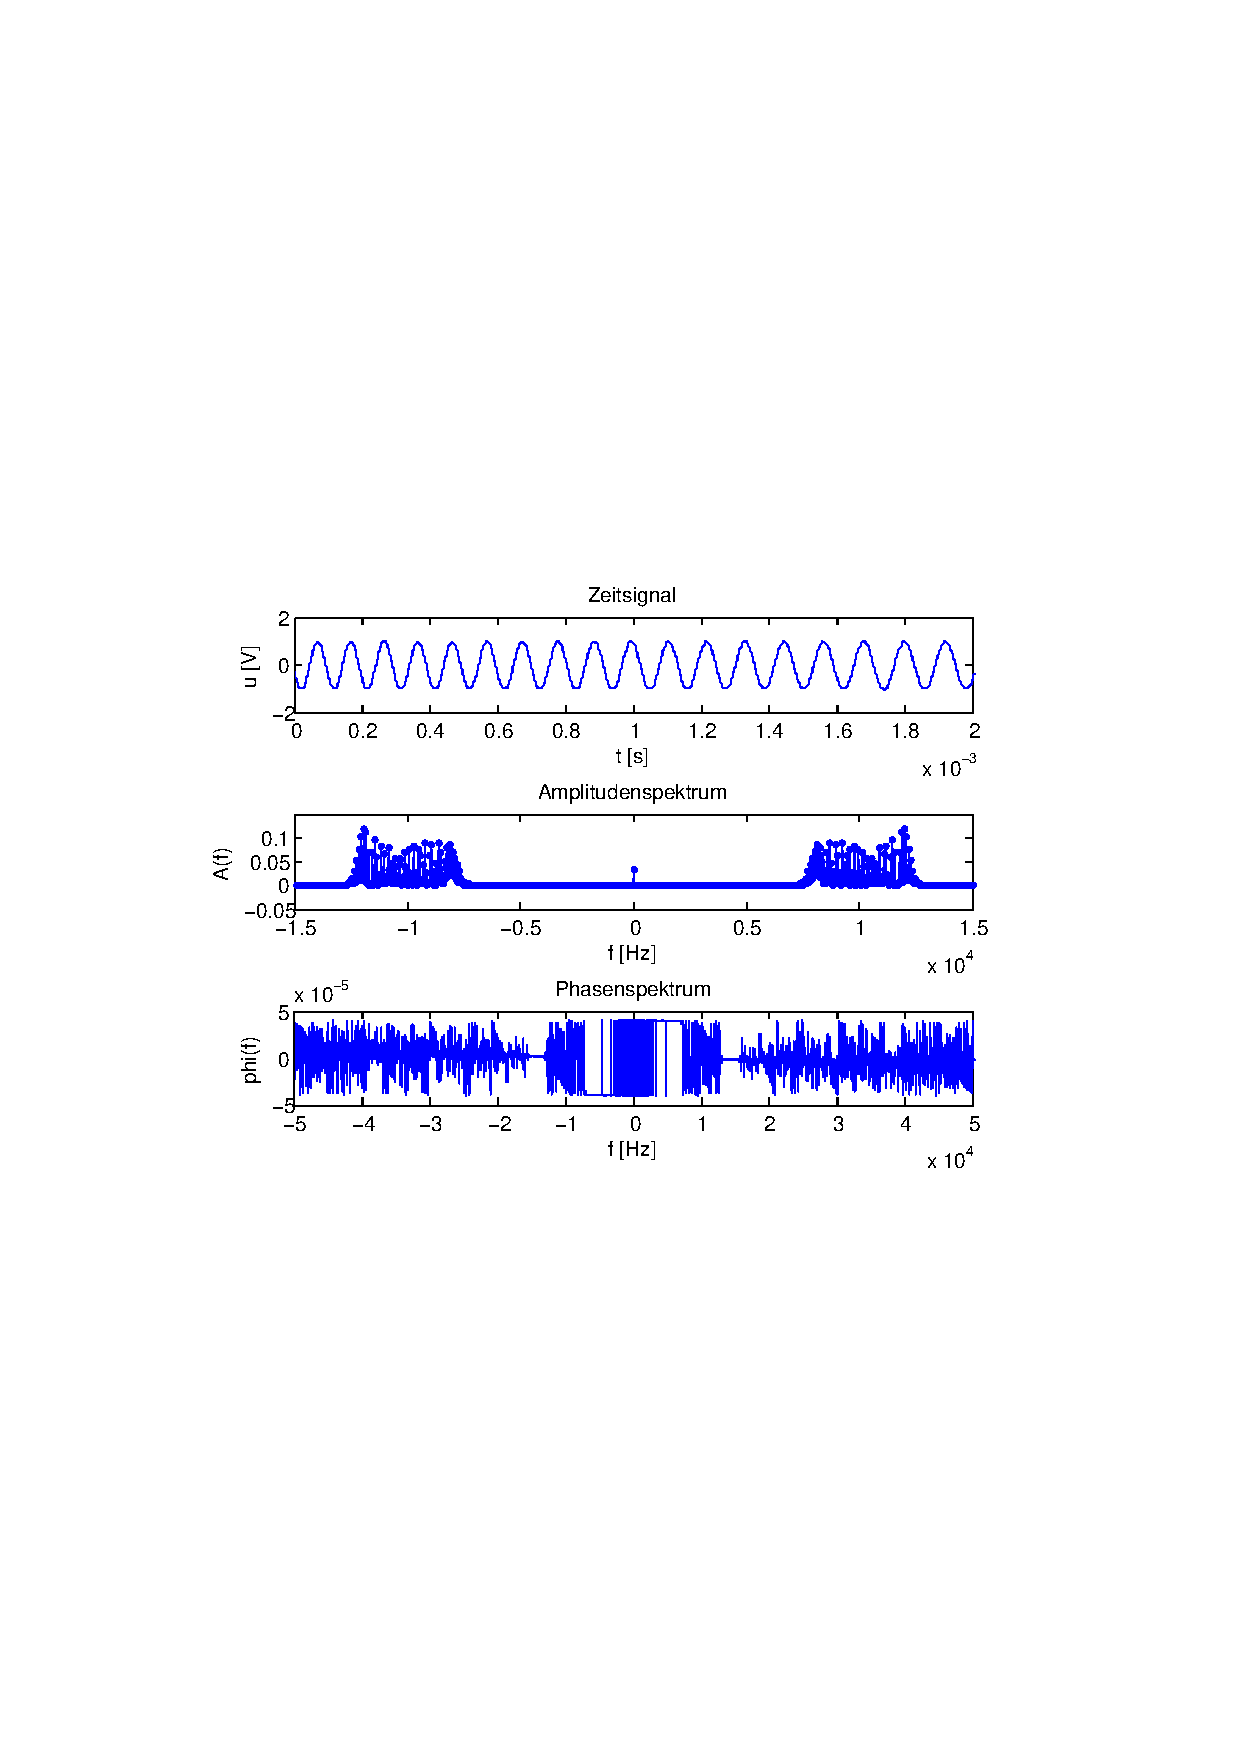
\includegraphics[scale=0.5, trim = 4cm 9.5cm 3.5cm
                        9.5cm, clip]{./Bilder/sin_a1_f100}
                        %FIXME [width=640px, height=474px]
                        \caption{Spektrum für moduliertes Sinusnutzsignal (1V,
                        100Hz)}
                    \end{figure}

                \end{minipage}
                \begin{minipage}{0.6\textwidth}

                     \begin{figure}[H]
                        \label{fig:}
                        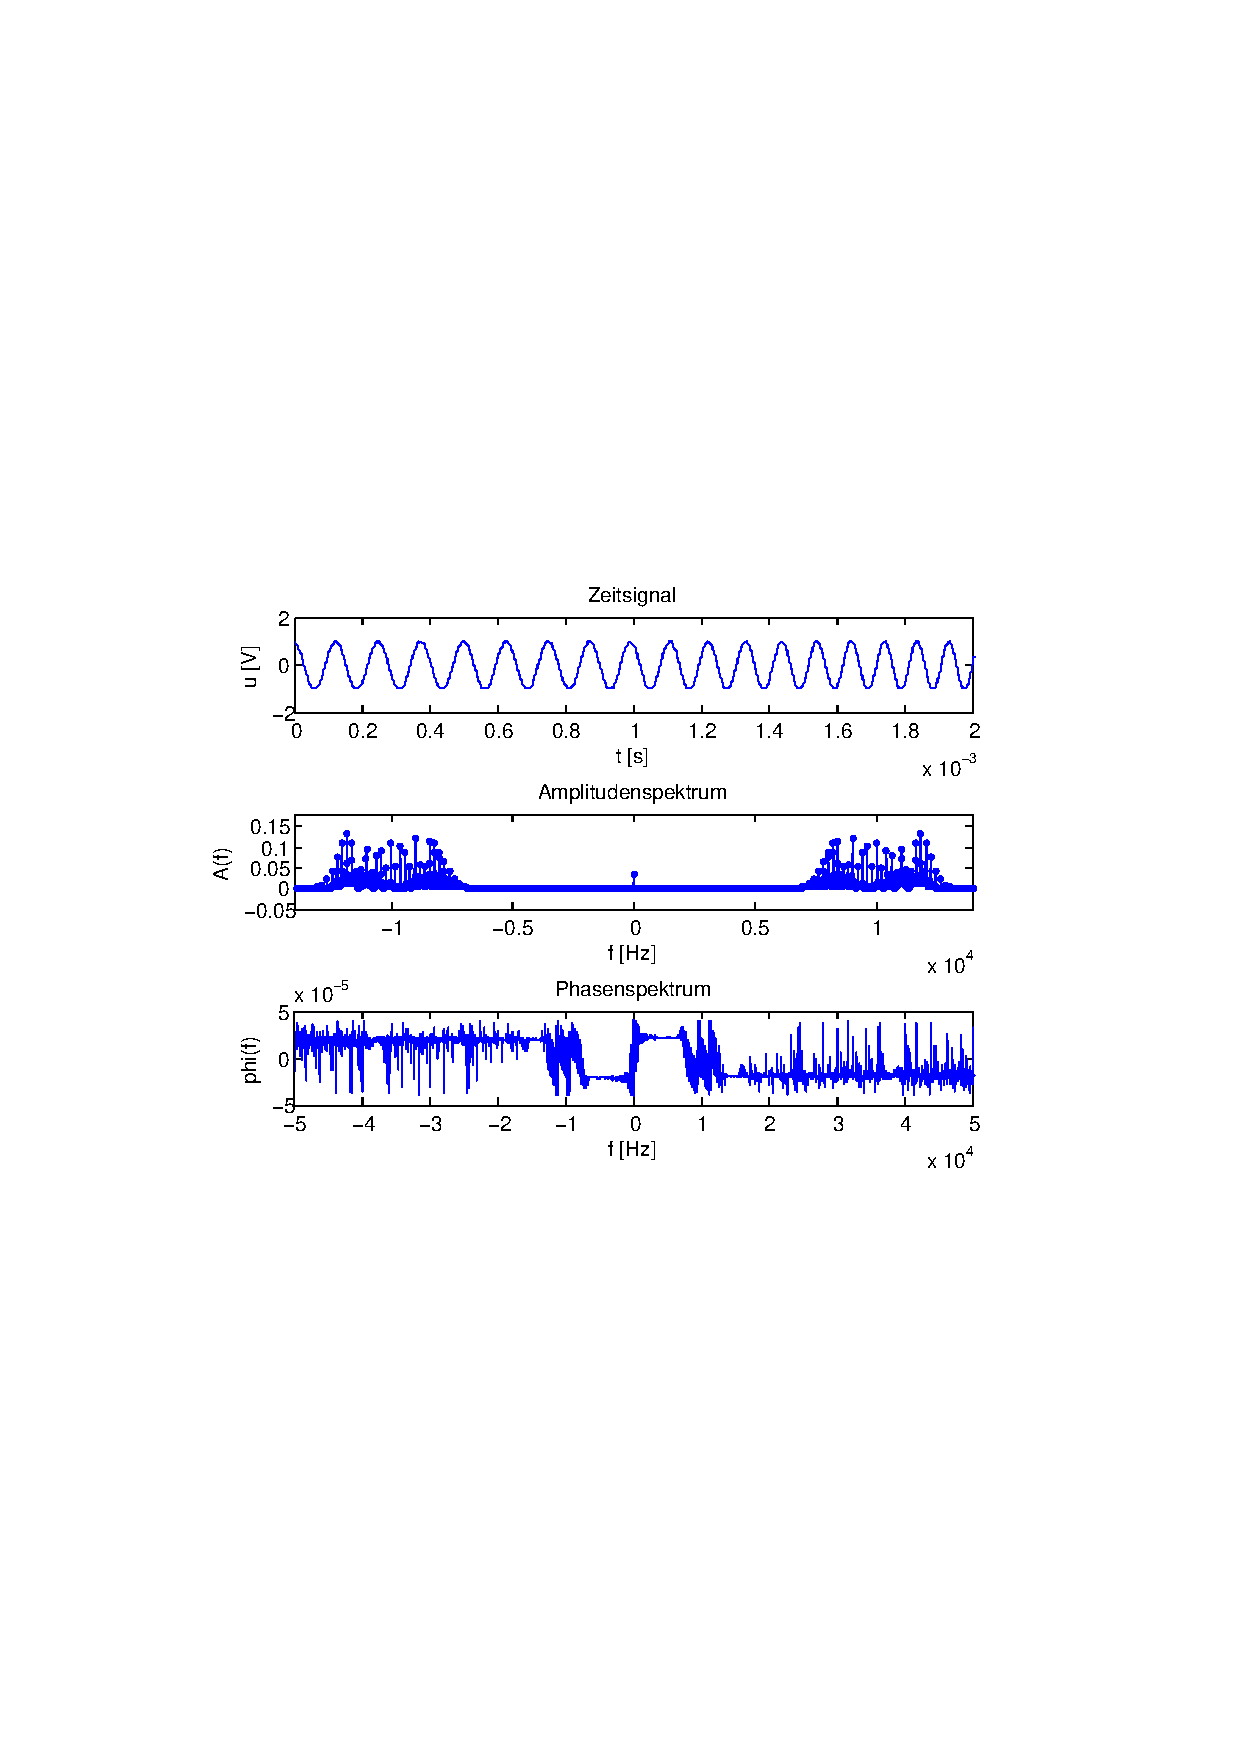
\includegraphics[scale=0.5, trim = 4cm 9.5cm 3.5cm
                        9.5cm, clip]{./Bilder/sin_a1_f200}
                        %FIXME [width=640px, height=474px]
                        \caption{Spektrum für moduliertes Sinusnutzsignal (1V,
                        200Hz)}
                    \end{figure}
               \vspace{-1.5em}

                \end{minipage}

            \end{tabular}
            \end{center}
        
        %Dreitte Reihe mit 2 Bildern
        
               \begin{center}
            \begin{tabular}{ll}

            \hspace{-10em}
                \begin{minipage}{0.6\textwidth}

                    \begin{figure}[H]
                        \label{fig:}
                        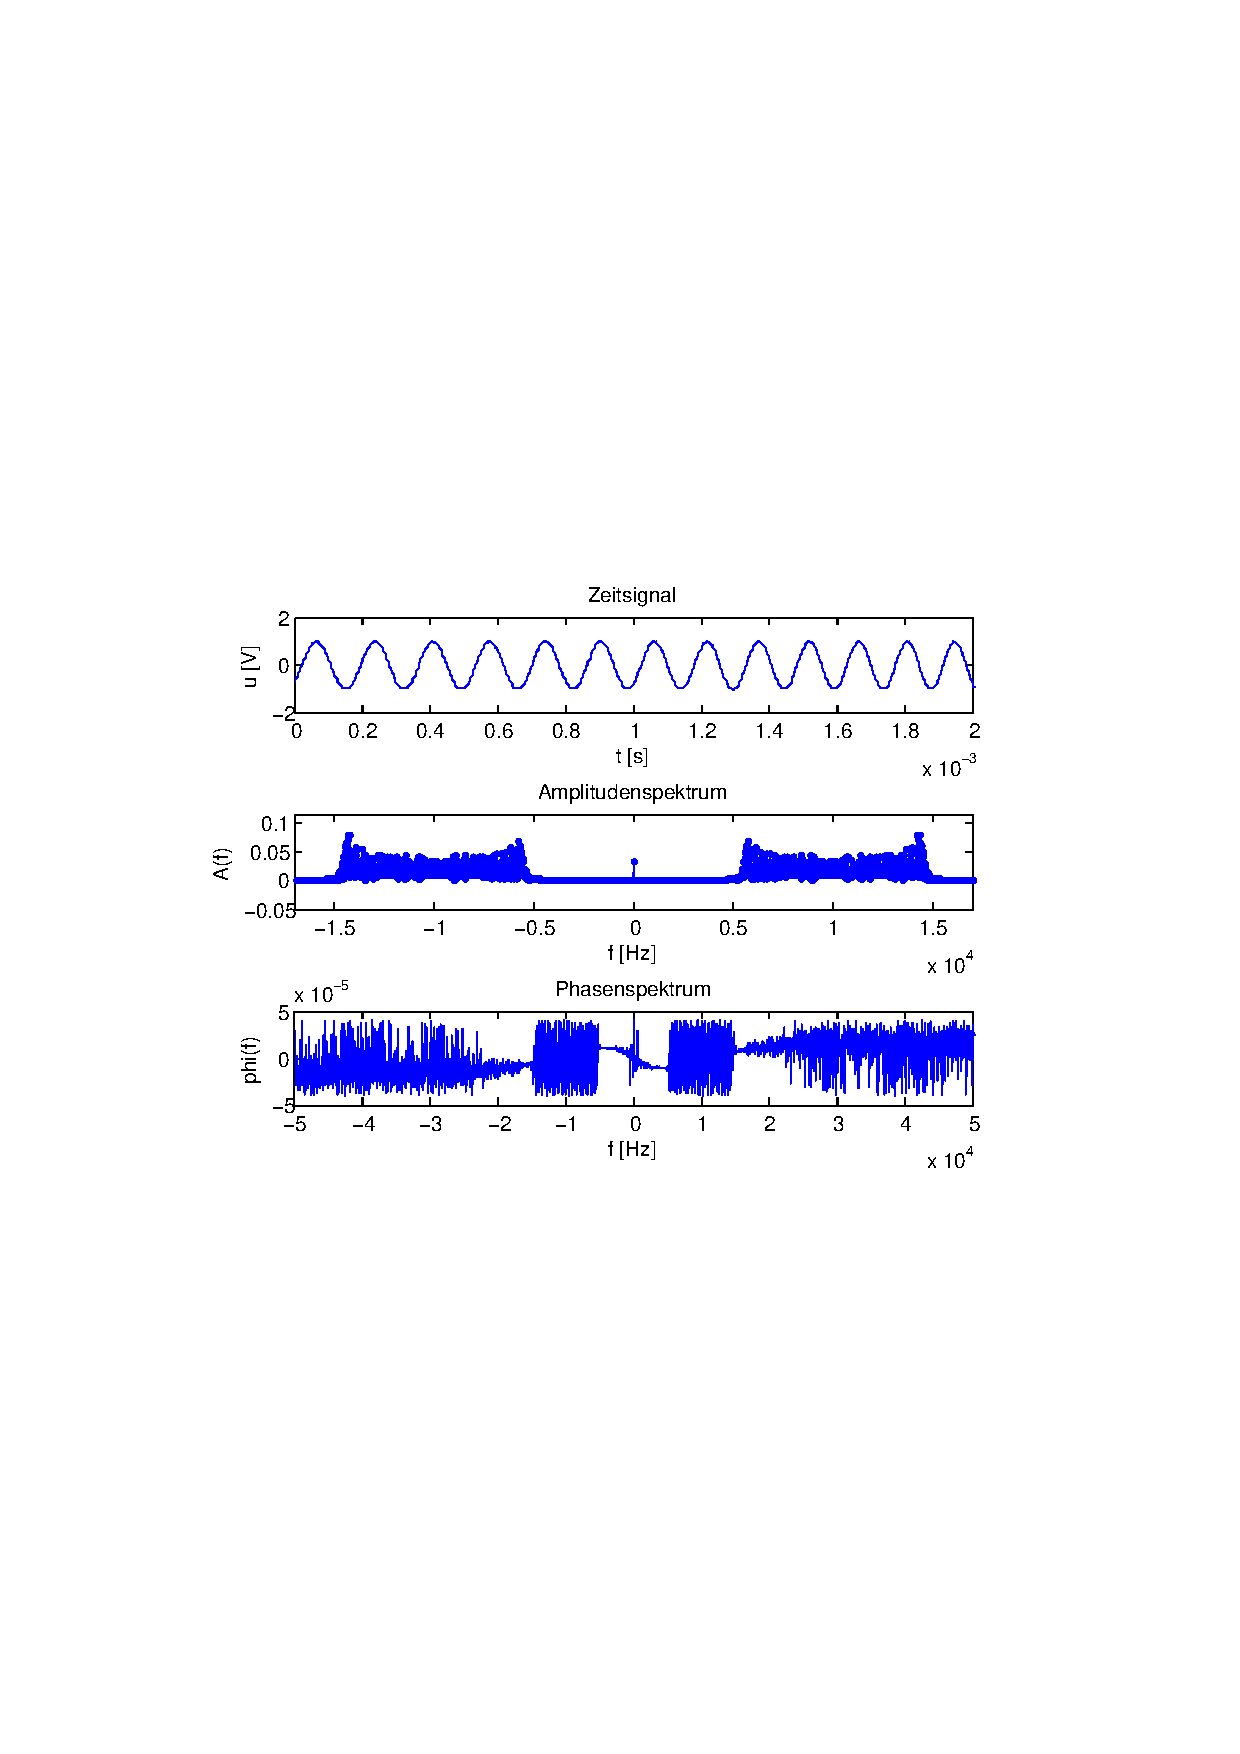
\includegraphics[scale=0.5, trim = 4cm 9.5cm 3.5cm
                        9.5cm, clip]{./Bilder/sin_a2_f50}
                        %FIXME [width=640px, height=474px]
                        \caption{Spektrum für moduliertes Sinusnutzsignal (2V,
                        50Hz)}
                    \end{figure}

                \end{minipage}
                \begin{minipage}{0.6\textwidth}

                     \begin{figure}[H]
                        \label{fig:}
                        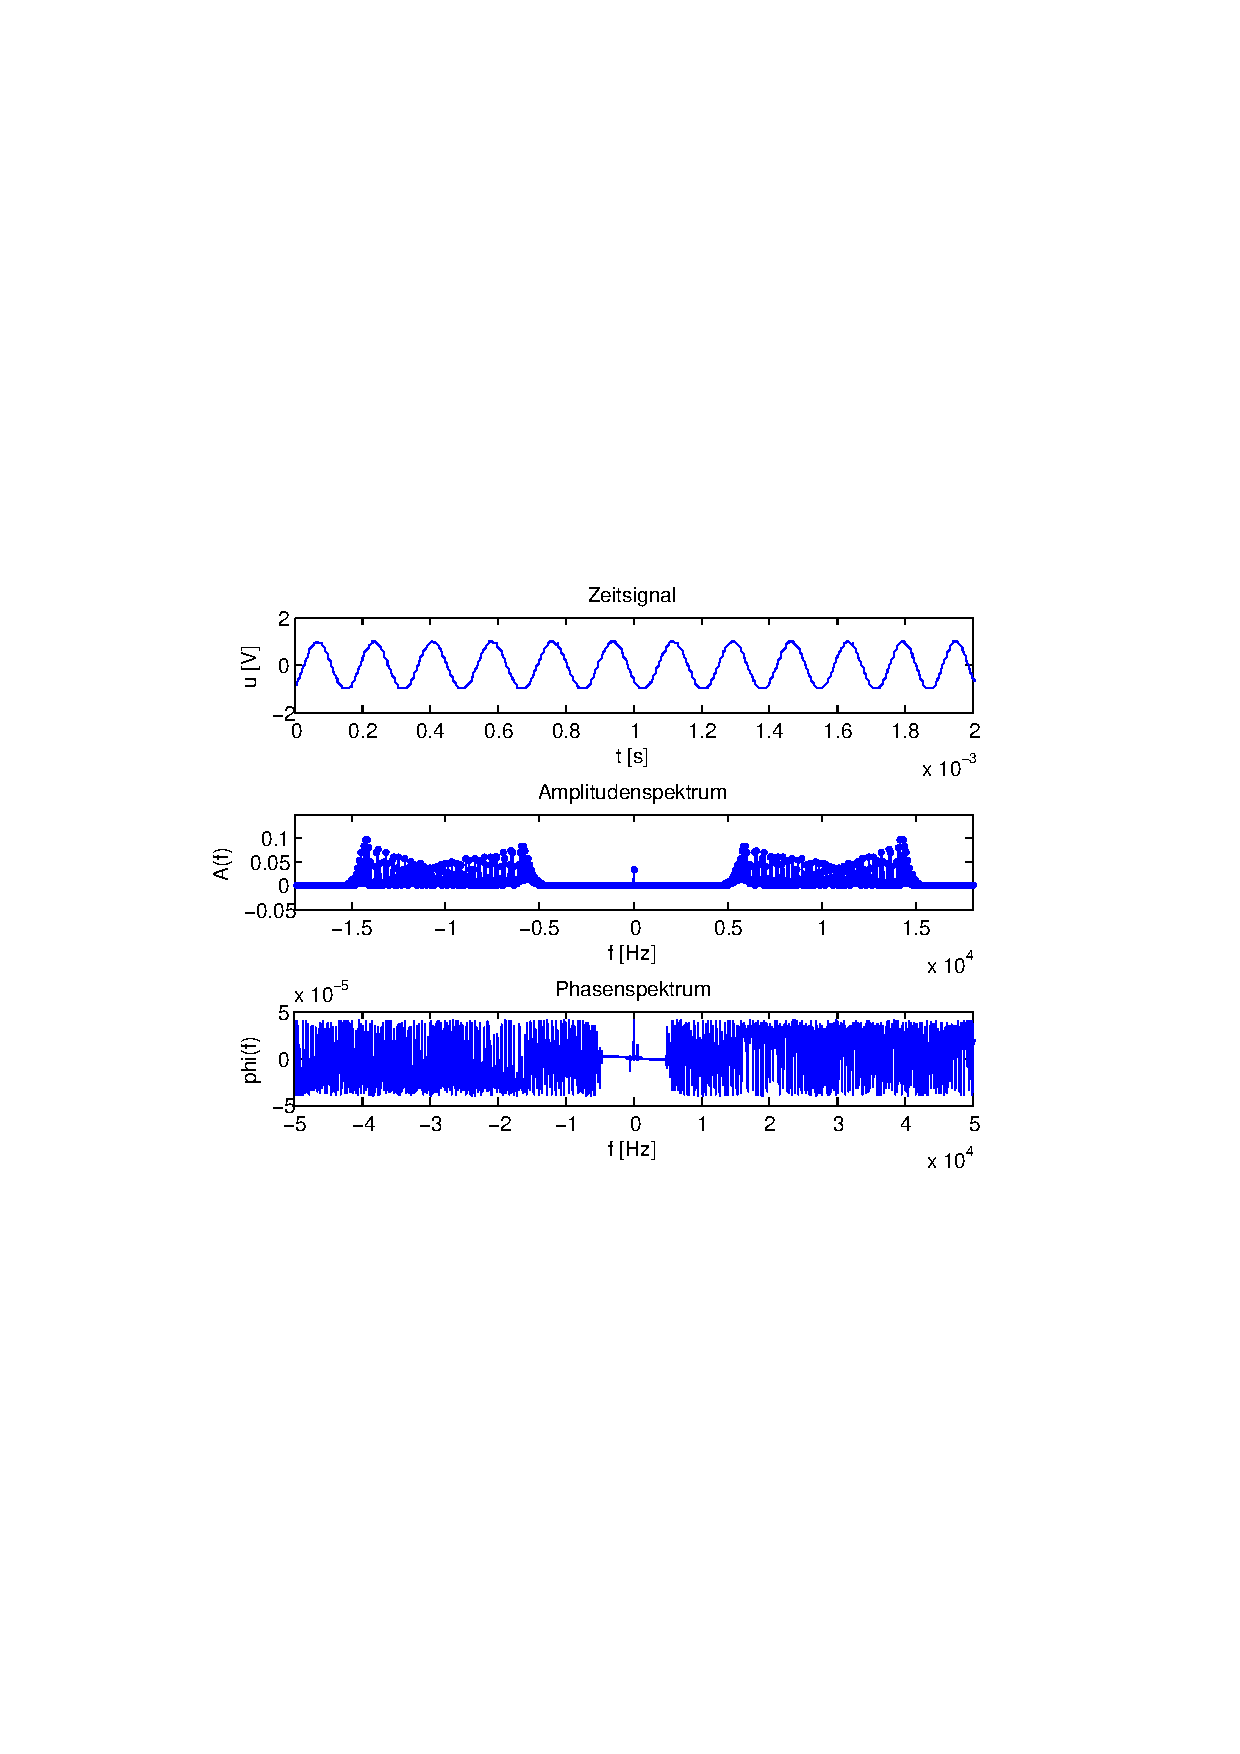
\includegraphics[scale=0.5, trim = 4cm 9.5cm 3.5cm
                        9.5cm, clip]{./Bilder/sin_a2_f100}
                        %FIXME [width=640px, height=474px]
                        \caption{Spektrum für moduliertes Sinusnutzsignal (2V,
                        100Hz)}
                    \end{figure}
               \vspace{-1.5em}

                \end{minipage}

            \end{tabular}
            \end{center}
            
            %Vierte Reihe mit nur einem Bild
            
             \begin{figure}[H] \centering
                    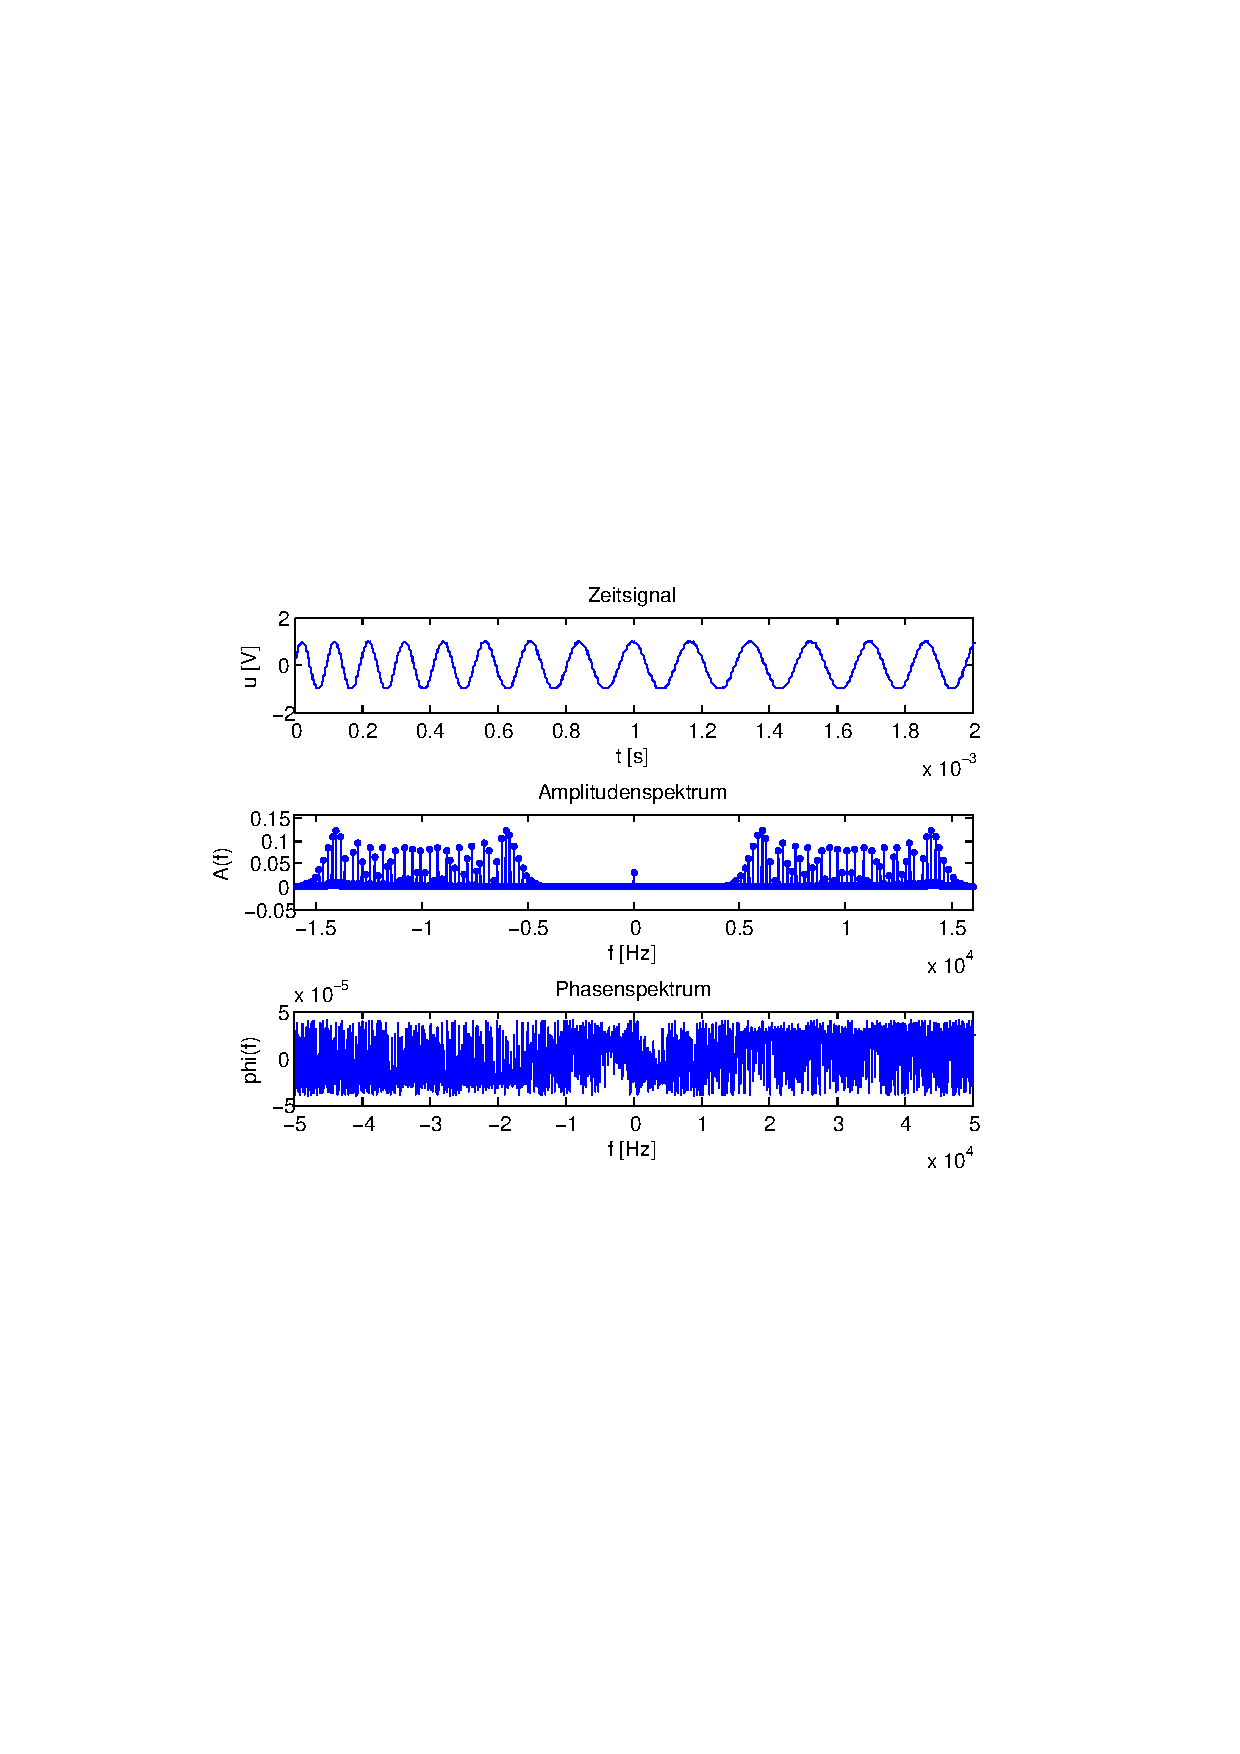
\includegraphics[scale=0.5, trim = 4cm 9.5cm 3.5cm
                        9.5cm, clip]{./Bilder/sin_a2_f200}
                        \caption{Spektrum für moduliertes Sinusnutzsignal (2V,
                        200Hz)}
                \end{figure}
            
            
            An den Unterschiedlichen Spektren lässt sich eine Tendenz
            entdecken. Beispielsweise an den Spektren mit der
            Eingangssignalamplitude $0.5 V$. Dabei lässt sich erkennen, dass die Amplitude 
            der Impulse im Betragsspektrum mit wachsender Frequenz höher werden. An der
            Stelle in der Frequenzachse ändert sich dabei nichts. Die gleiche
            Beobachtung kann man auch mit der Messreihe der Nutzsignale mit der
            Amplitude $1V$ und $2V$ machen. Die wachsende Amplitude dagegen
            bewirkt, dass die auftretenden Impulsgruppen breiter werden und mehr
            Frequenzen benötigen. Somit kann man abschließend zusammenfassen,
            dass die steigende Amplitude des Nutzsignals im modulierten Spektrum
            zu einer höheren Amplitude und die wachsende Frequenz zu einem
            breiteren Freuquenzband führt.
           
       \end{quote}
            
  	     \subsubsection{FM-Demodulation}
           \begin{quote}
            
            Bei der FM-Demodulation wurde das Comparator- und das Twin Pulse
            Generator-Modul eingesetzt. Die Funktion beider Module wurde bereits
            in der Durchführung ausreichend erläutert. Hier werden nun die
            Ausgänge der jeweiligen Module miteinander verglichen. Dabei gehen
            wir genauso vor, wie auch in der Durchführung.\\
            Als erstes wird bei fester Sendesignalfrequenz der Comparatorausgang
            betrachtet:
            
            
             \begin{figure}[H] \centering
                    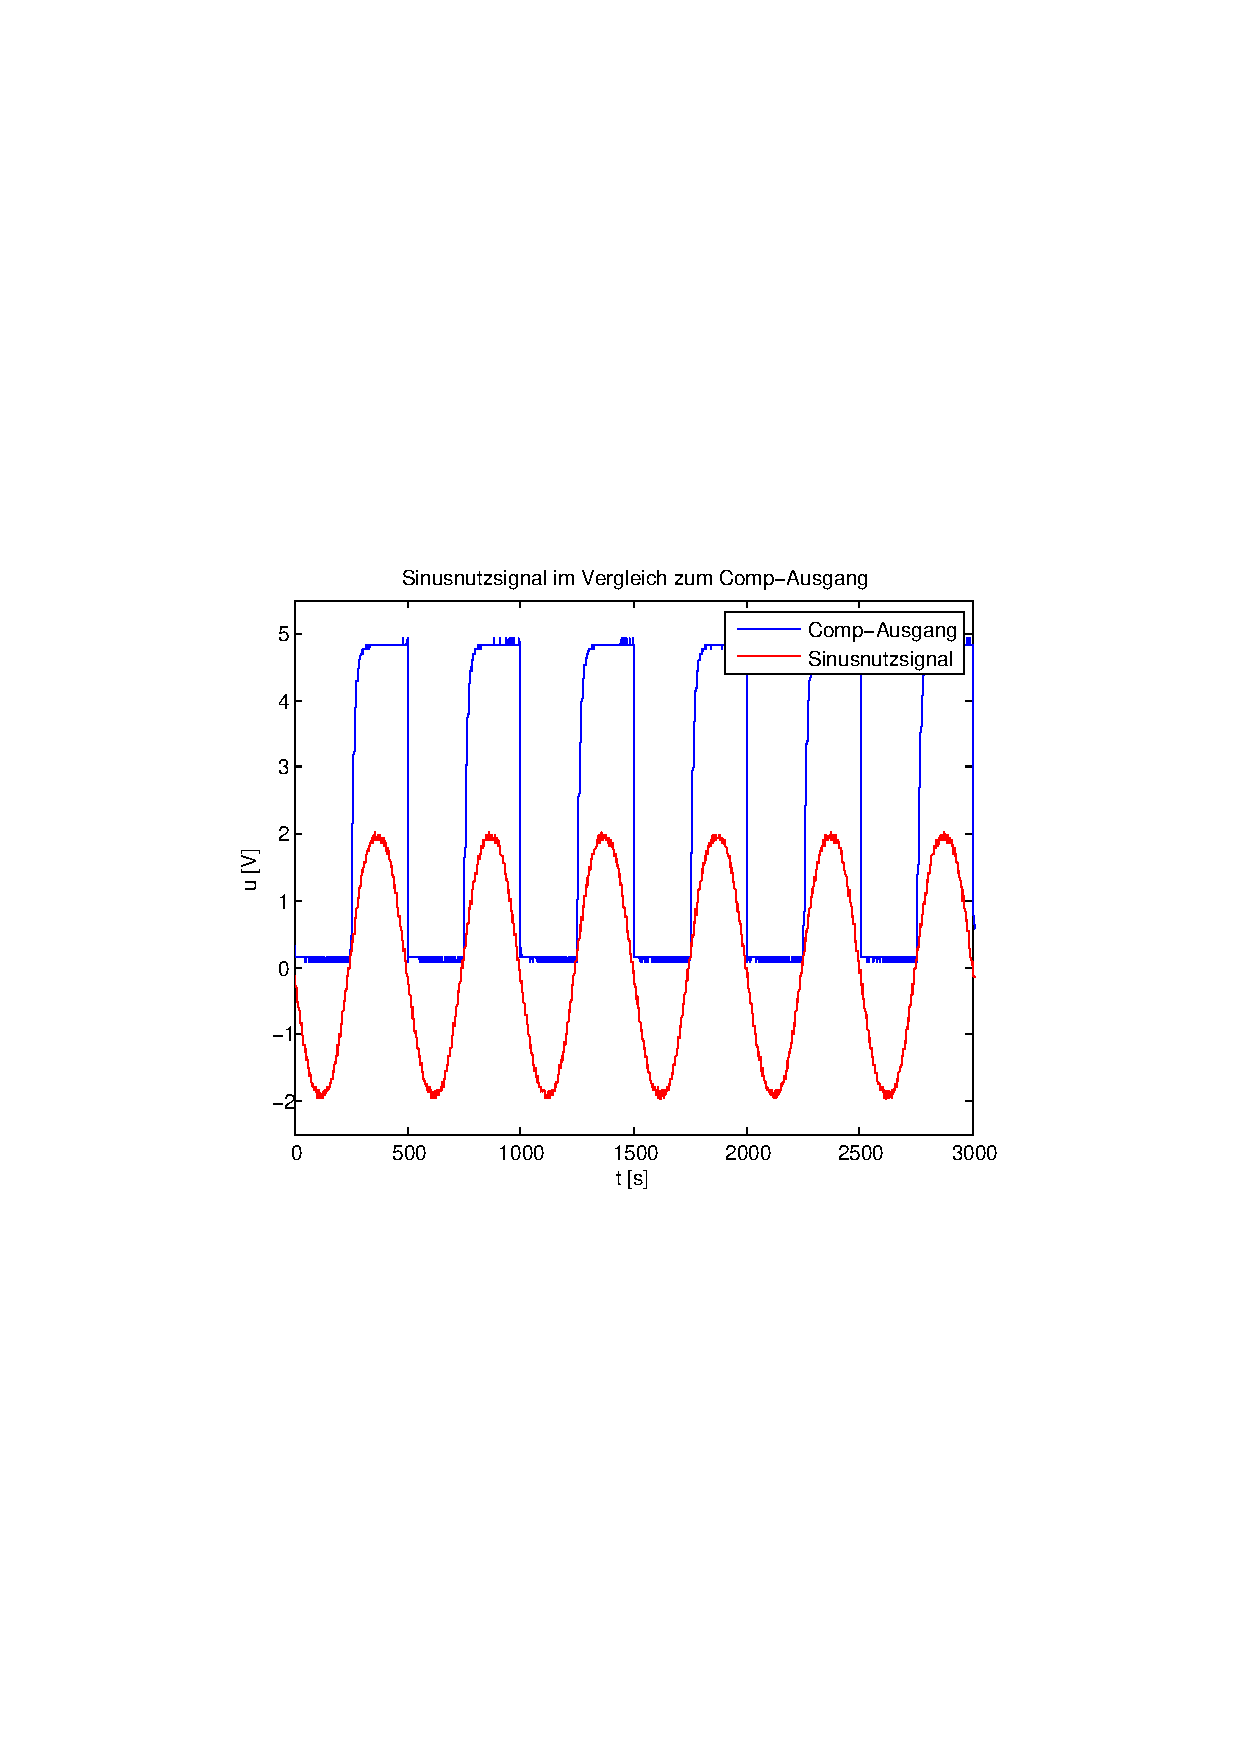
\includegraphics[scale=0.5, trim = 4cm 9.5cm 3.5cm 9.5cm,
                    clip]{./Bilder/sin_vs_comp}
                        \caption{Vergleich zwischen festem Sendesignal und
                        Signalverlauf am Comparator}
                \end{figure}          
            

           
            
           Hier kann man sehr genau die Funktion des Comparator erkennen. Da wir
           einen Sinus ohne Offset verwenden und die verwendete Referenzspannung
           $0V$ beträgt, wird der Comp-Ausgang wie erwartet auf das high Signal 
           gesetzt, sobald das Sendesignal vom negativen in den positiven
           Bereich übergeht. Im umgekehrten Fall wird der Comp-Ausgang auf low
           gesetzt. Somit entspricht diese Messung unseren Erwartungen.\\
           Als nächstes werden Sendesignal und TPG-Ausgang in den Vergleich
           gesetzt:
             
             \begin{figure}[H] \centering
                    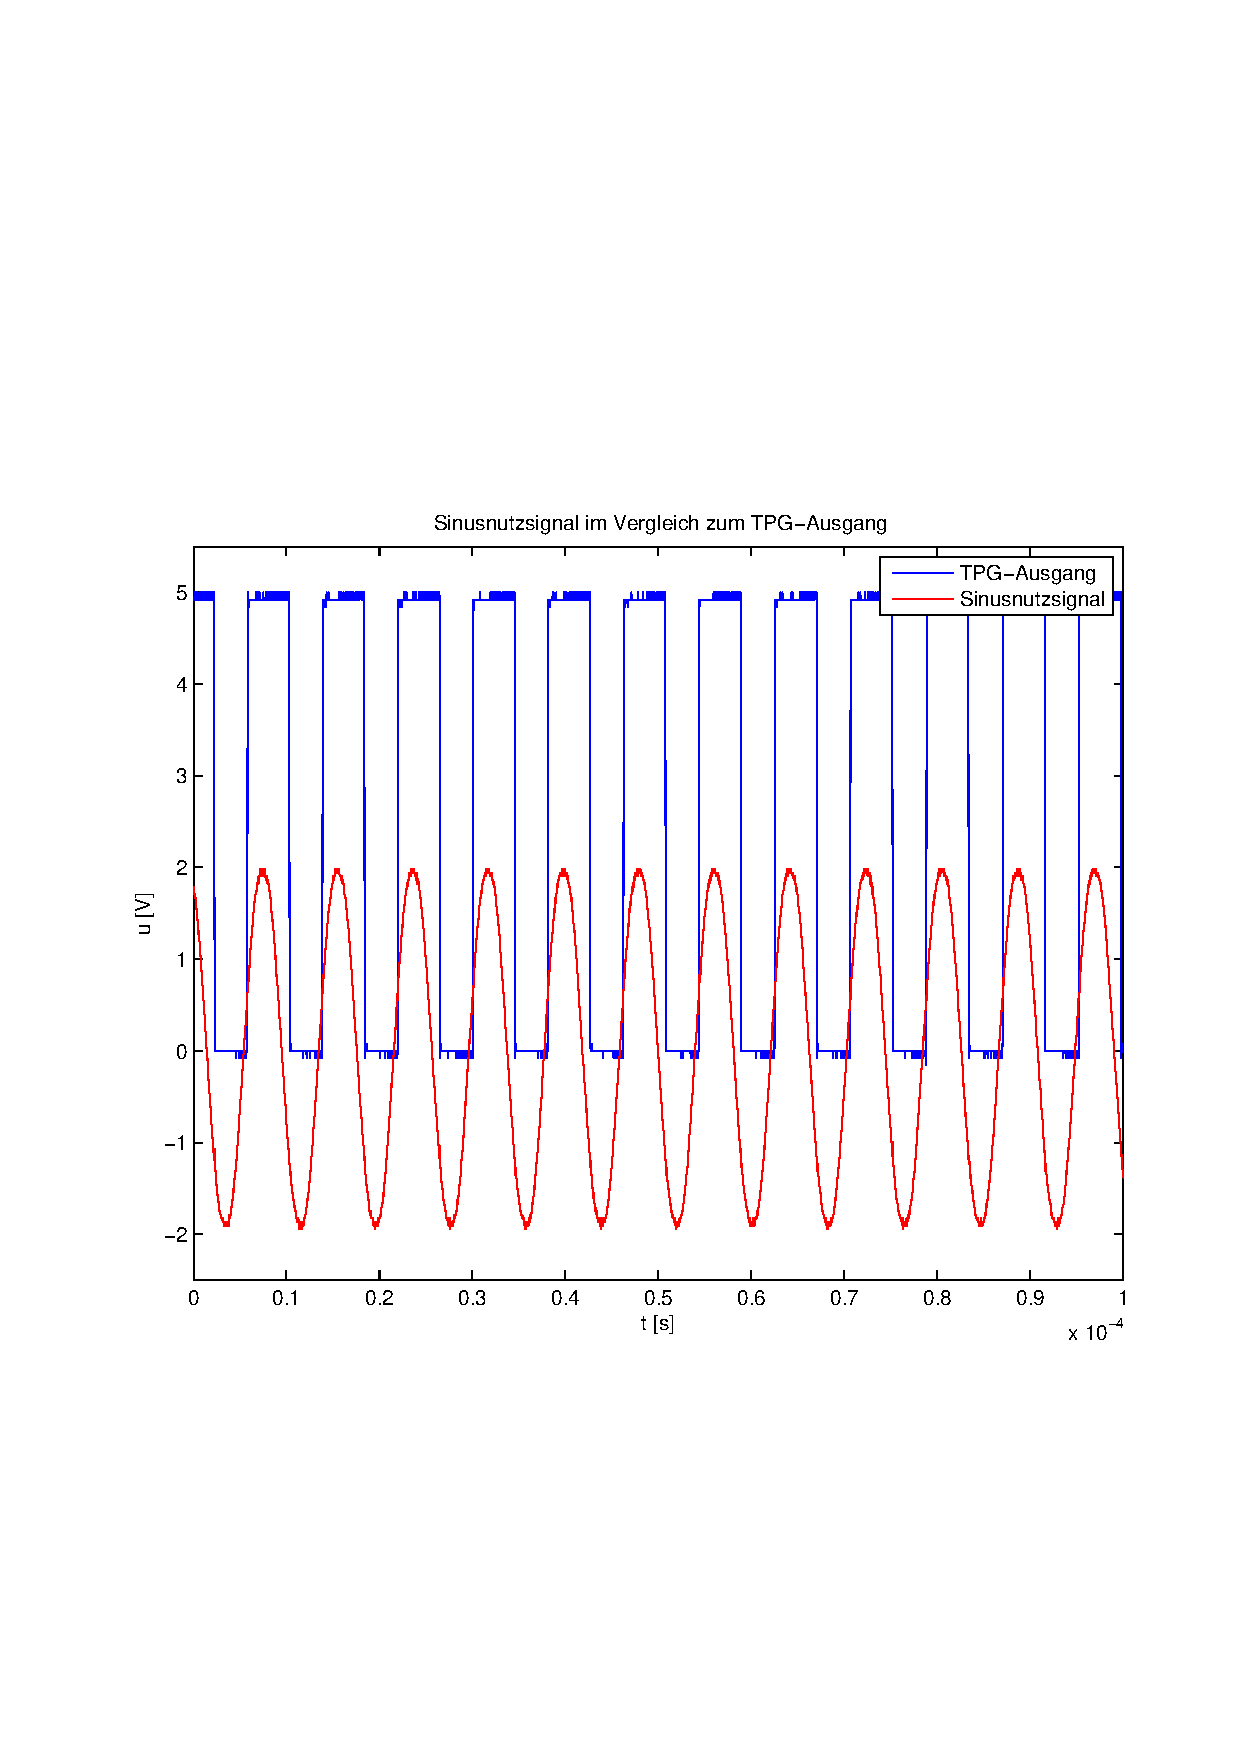
\includegraphics[scale=0.5, trim = 4cm 9.5cm 3.5cm 9.5cm,
                    clip]{./Bilder/sin_vs_tpg}
                        \caption{Vergleich zwischen festem Sendesignal und
                        Signalverlauf am TPG}
                \end{figure}
           
           
           \TODO{TPG genauer erklären}
           
           An diesem Ergebnis können wir sehen, dass der TPG-Ausgang und der
           Comp-Ausgang fast das gleiche Signal liefern. Auch dies entspricht
           unseren Erwartungen, da der TPG bei jeder steigenden Flanke ein
           einzelnes Deltaimpuls ausgibt. Ungefähr $8ms$ nach diesem Deltaimpuls
           wird ein weiterer Deltaimpuls ausgegeben (daher Twin-Pulse). Grafisch
           dargestellt sieht dies auf dem Oszilloskop wie ein Rechtecksignal
           aus. Dass die Rechtecke des Comparator und die quasi Rechtecke Des
           TPG ca. die gleiche Breite aufweisen, ist ein Zufall, dass durch die
           Frequenz des Sendesignals entstanden ist. Daher macht es grafisch
           den Eindruck, dass der TPG ein Rechtecksignal über das
           Rechtecksignal des Comparators legt. Ein kleiner Unterschied ist aber
           im Delay bemerkbar.
           Da der TPG erst nach dem Comp vom Signal durchlaufen wird, ist
           dieses kleine Delay zwischen festem Sendesignal und dem
           TPG-Ausgangssignal nicht überraschend.\\
           
           \vspace{0.5em}
           
           Dass der Comparator und der TPG fast das gleiche Signal ausgeben,
           wird nochmal im Vergleich ihrer Ausgangssignale deutlich:
           
            
             \begin{figure}[H] \centering
                    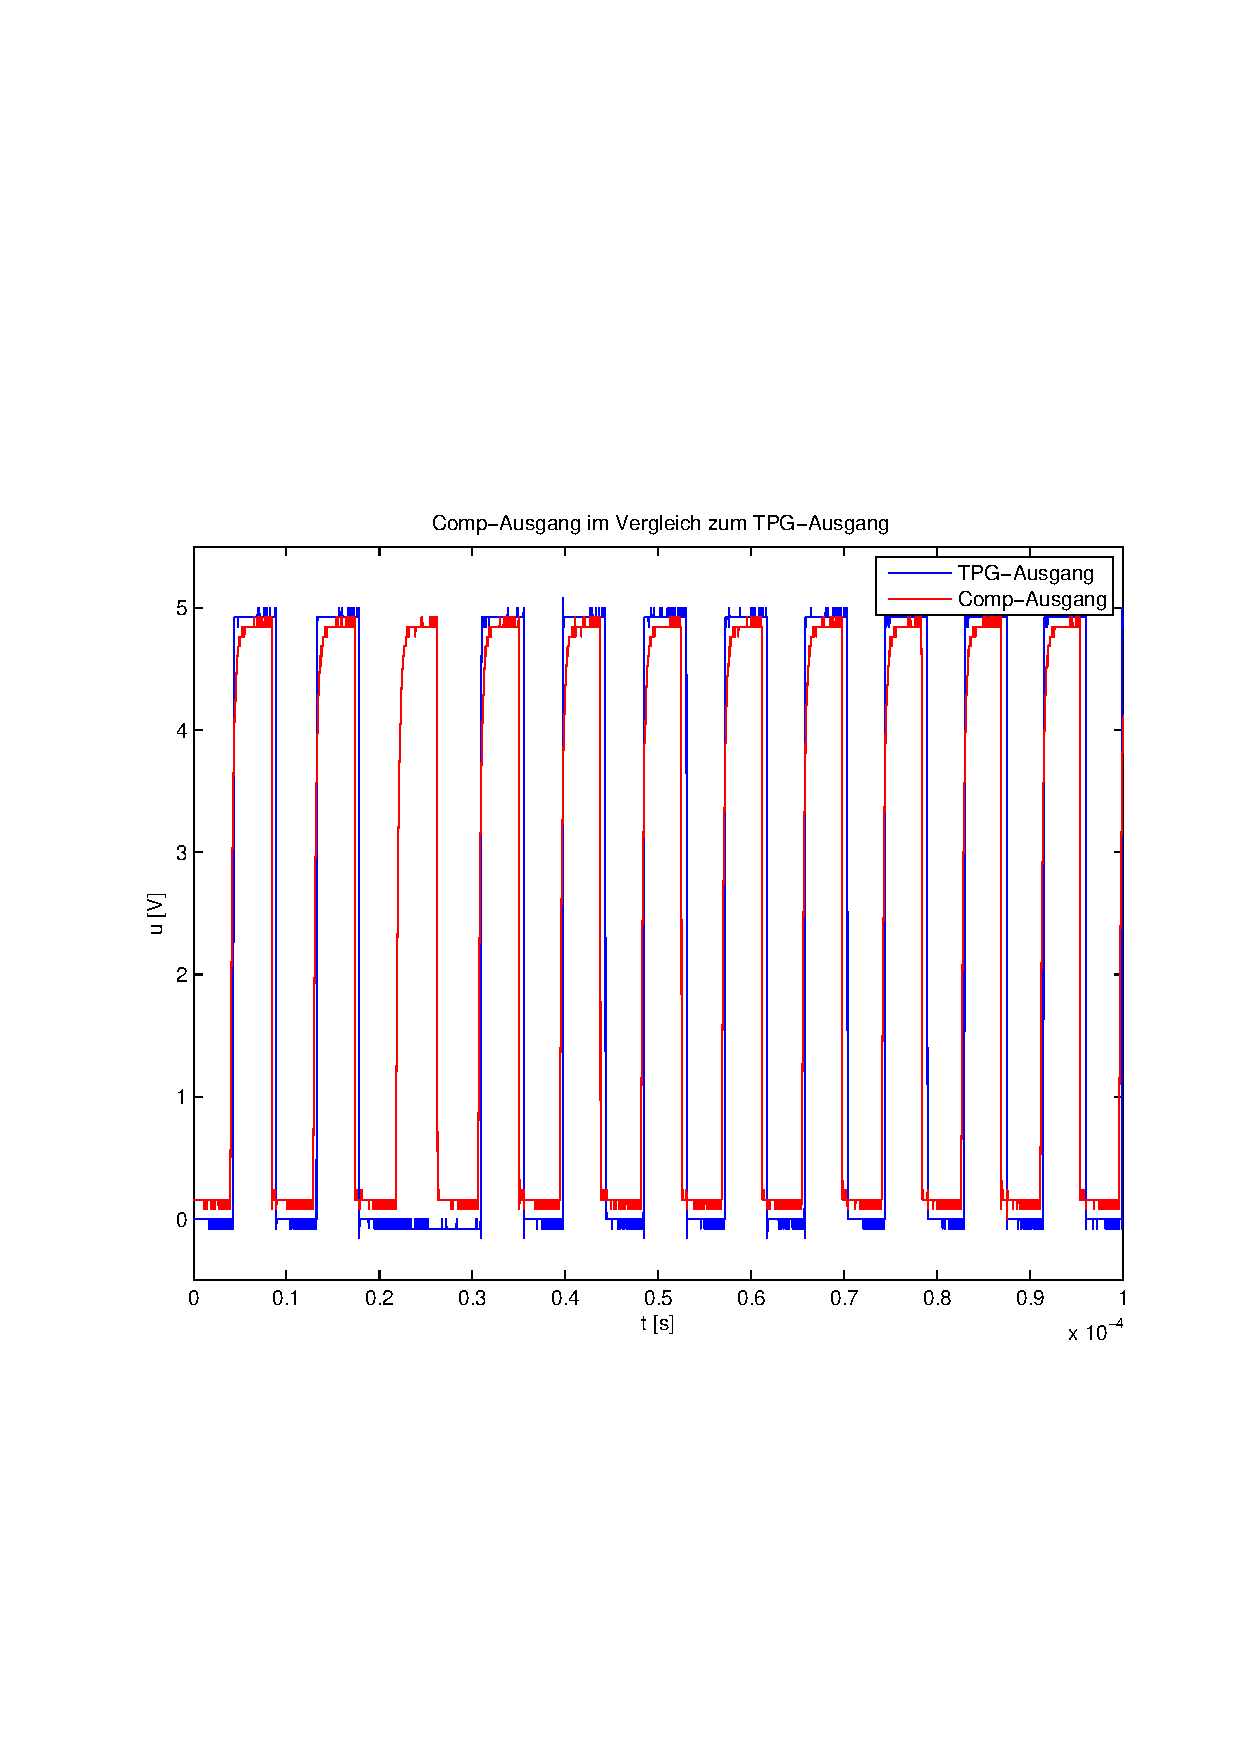
\includegraphics[scale=0.5, trim = 4cm 9.5cm 3.5cm 9.5cm,
                    clip]{./Bilder/comp_vs_tpg}
                        \caption{Vergleich zwischen Comparator- und
                        TPG-Ausgangssignal}
                \end{figure}
          
          Man kann deutlich sehen, dass beide Ausgänge einen sehr ähnlichen
          Verlauf haben, der TPG aber manchmal nicht mit dem Comp-Ausgang
          mitkommt und eine steigende Flanke überspringen kann, wodurch eine
          Störung in der Rechteckperiode entsteht.\\
          
          \vspace{0.5em}
          
          Zuletzt wurde das Sendesignal mit fester Frequenz in den Vergleich mit
          dem moduliert-demoduliertem Signal gesetzt. Das folgende Ergebnis kam
          heraus:
          
           
             \begin{figure}[H] \centering
                    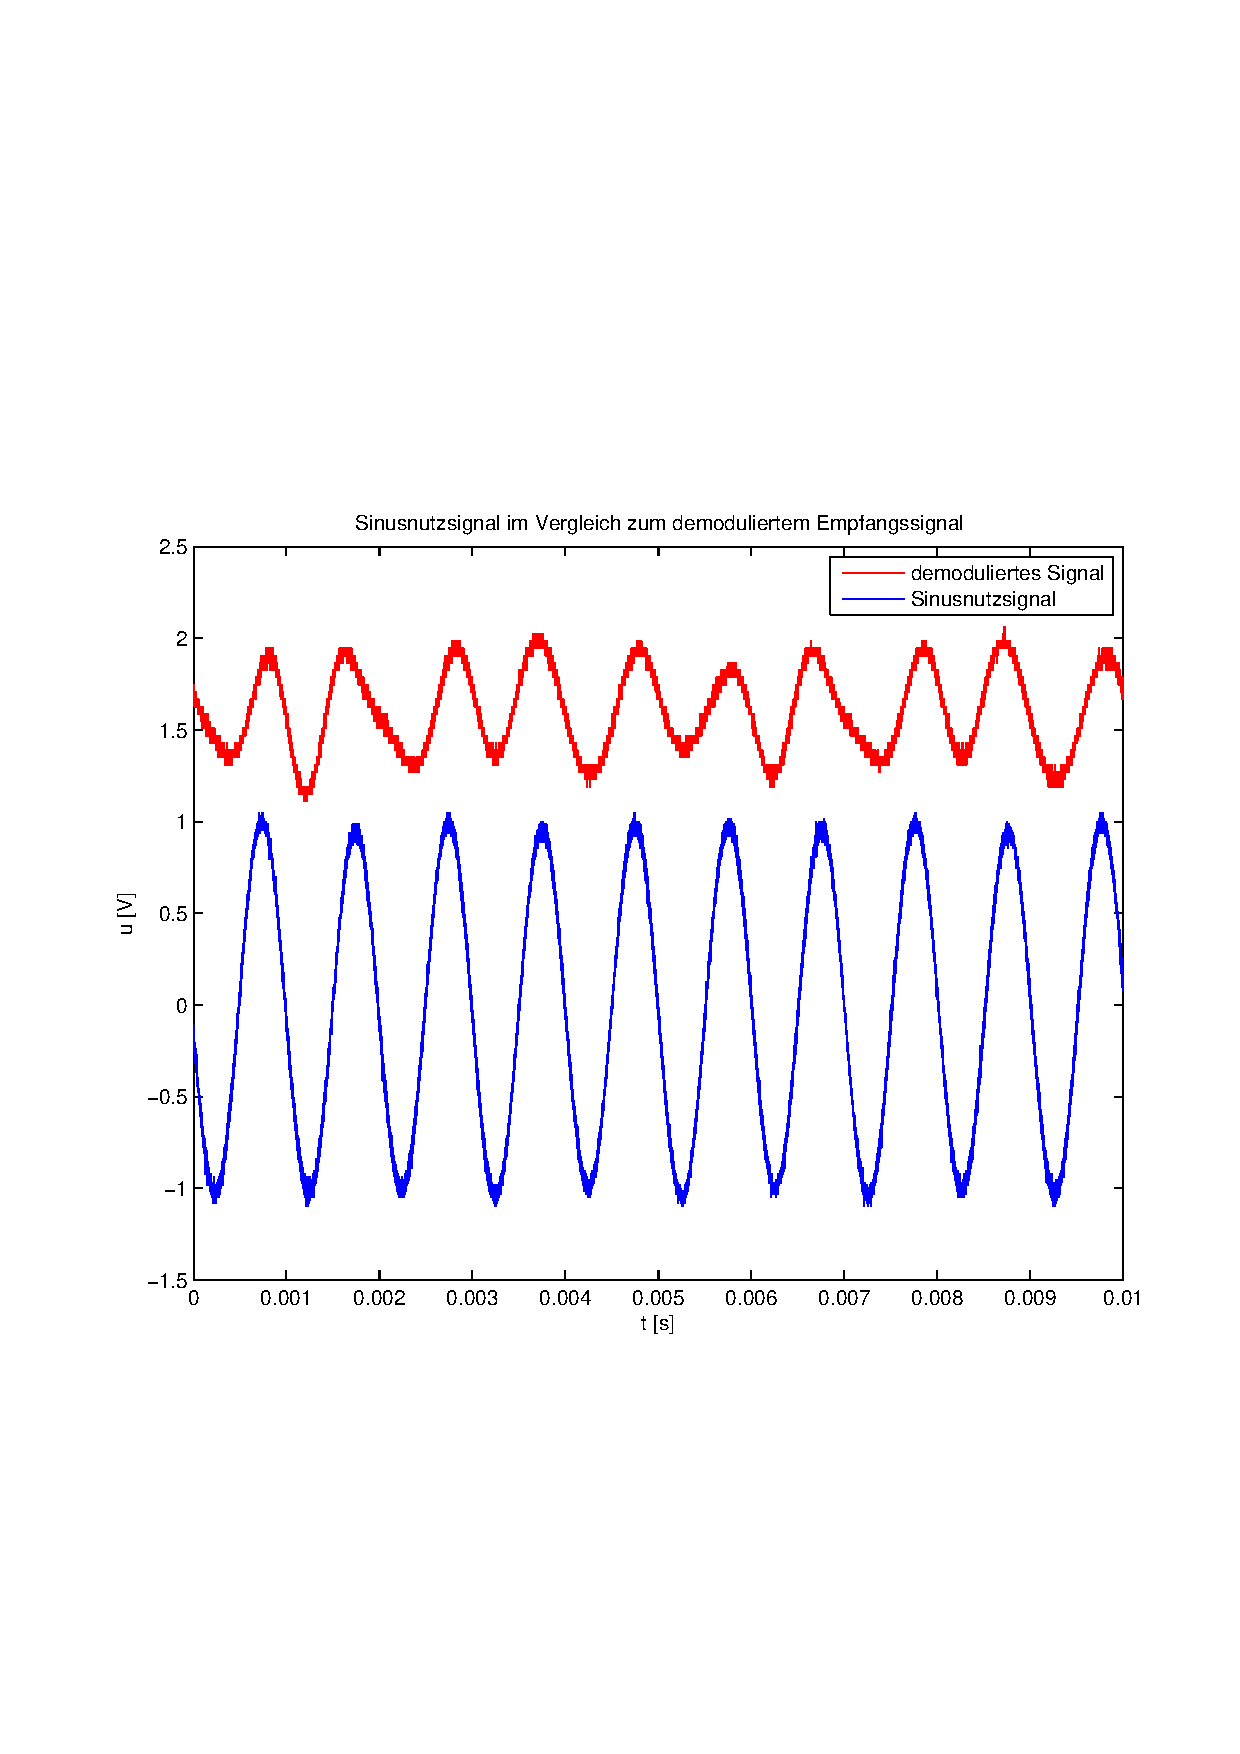
\includegraphics[scale=0.5, trim = 4cm 9cm 3.5cm 9.5cm,
                    clip]{./Bilder/sinus_fm_demod}
                        \caption{Vergleich zwischen festem Sendesignal und
                        demoduliertem Empfangssignal}
                \end{figure}
          
        Das demodulierte Signal besitzt einen Offset, keine korrekte Amplitude 
        und keinen sehr klaren Sinusverlauf. Diese Fehler können hauptsächlich
        dadurch entstehen, dass in unserer langen Kette an Modulen für die
        Demodulation bei jedem Schritt ein teil der Amplitude verloren gehen
        kann. Dies geschieht zum Beispiel, wenn durch die hohe
        Sendesignalfrequenz der Comparator und der TPG steigende Flanken
        verpassen und kein korrektes Ausgangssignal weitergeben. Somit kann sich
        der Fehler in den weiteren Modulen fortsetzen und vergrößern, was sich
        dann am demodulierten Empfangssignal bemerkbar macht.\\
               
        Daraus lässt sich schließen, dass die FM-PFM-Umwandlung
        für eine FM-Demodulation eines Sinussignals nicht sehr geeignet ist.\\
        
    	\end{quote}
    \end{quote}	
\end{quote}

%--------------------------------------------------------------------
%--------------------------------------------------------------------    

\section{Zusammenfassung}
\begin{quote}
	
\end{quote}

%--------------------------------------------------------------------
%--------------------------------------------------------------------    


\begin{thebibliography}{999}
\bibitem {AMohnetraeger} Prof. Dr.-Ing. Sikora, Thomas; Prof. Dr.-Ing. Noll, Peter: Einführung in die
Nachrichtenübertragung, S.207
\bibitem {AMdemodulation} Prof. Dr.-Ing. Sikora, Thomas; Prof. Dr.-Ing. Noll, Peter: Einführung in die
Nachrichtenübertragung, S.209
\bibitem {AMohneUeber} Prof. Dr.-Ing. Sikora, Thomas; Prof. Dr.-Ing. Noll, Peter: Einführung in die
Nachrichtenübertragung, S.206
\bibitem {AMmitUeber} Prof. Dr.-Ing. Sikora, Thomas; Prof. Dr.-Ing. Noll, Peter: Einführung in die
Nachrichtenübertragung, S.215



%Name, Vorname.; evtl. Name2, Vorname2.: Titel des Dokumentes
%oder Buches, Zeitschrift/Verlag/URL (Auflage, Erscheinungsort, -jahr), ggf. Seitenzahlen
% \bibitem {PasevalscheTheorem} \url{https://de.wikipedia.org/wiki/Parsevalsches_Theorem}, Zugriff
% 23.05.2012
\end{thebibliography}

\end{document}
